\clearpage

\section{Geometric calibration and command generation}

\subsection{A known machine as a numerical control}

Start with a machine whose error maps are known exactly. This isolates errors in coordinate transformations and in the inverse command calculation. On the reference helix the uncorrected TCP RMS is 122.44 micrometres. Restricting the correction to five positioning channels increases it to 126.49. With the full known map the residual falls to numerical tolerance. Removing one component can undo cancellation with another.

\par{\small\textit{Implementation}\quad \file{fiveaxis.py}\enspace /\enspace \file{experiments.py}}\par

\begin{center}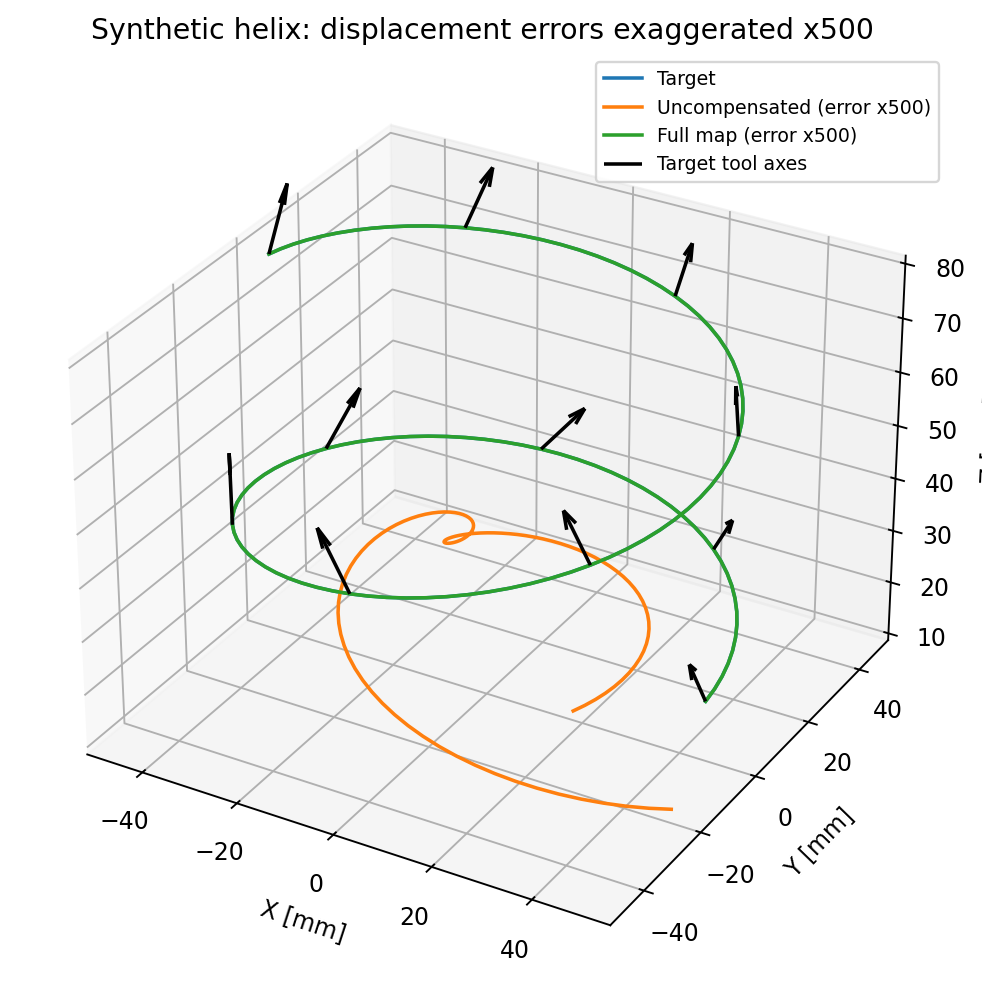
\includegraphics[width=.97\linewidth,height=73mm,keepaspectratio]{figures/helix_3d.png}\par\small\refstepcounter{figure}\textbf{Figure \thefigure.} The target and executed helix. Position differences are magnified 500 times for display.\end{center}

\begin{center}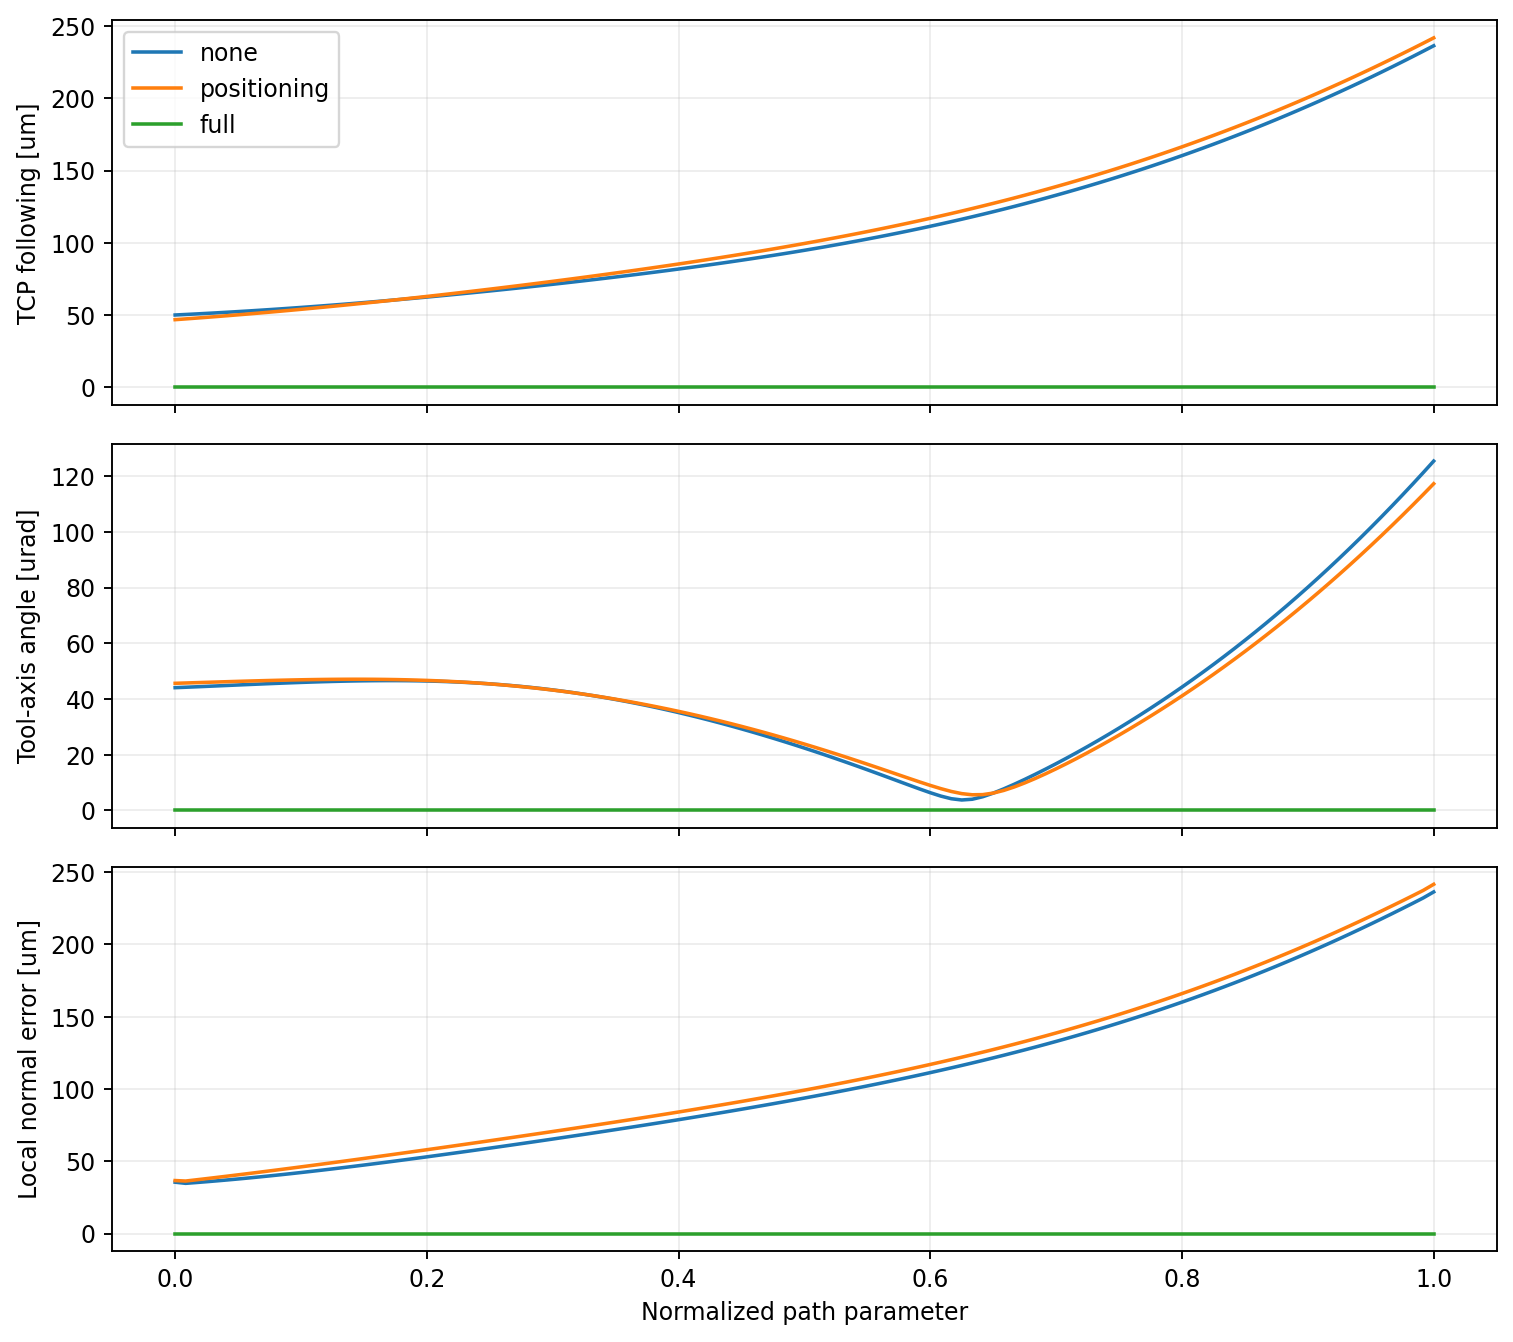
\includegraphics[width=.97\linewidth,height=73mm,keepaspectratio]{figures/geometry_compensation.png}\par\small\refstepcounter{figure}\textbf{Figure \thefigure.} TCP magnitude, axis direction and normal-plane error on the same commands.\end{center}

\clearpage

\subsection{From an axis map to a spatial error field}

An error map is referenced to a datum. Translating the part-coordinate origin changes the map evaluated at a given part position. The spatial map then holds both rotary angles fixed and samples 343 linear-axis poses. A colour records the simulated displacement norm at one pose. A single slice cannot establish a worst case for all rotary configurations.

\par{\small\textit{Implementation}\quad \file{fiveaxis.py}\enspace /\enspace \file{experiments.py}}\par

\begin{center}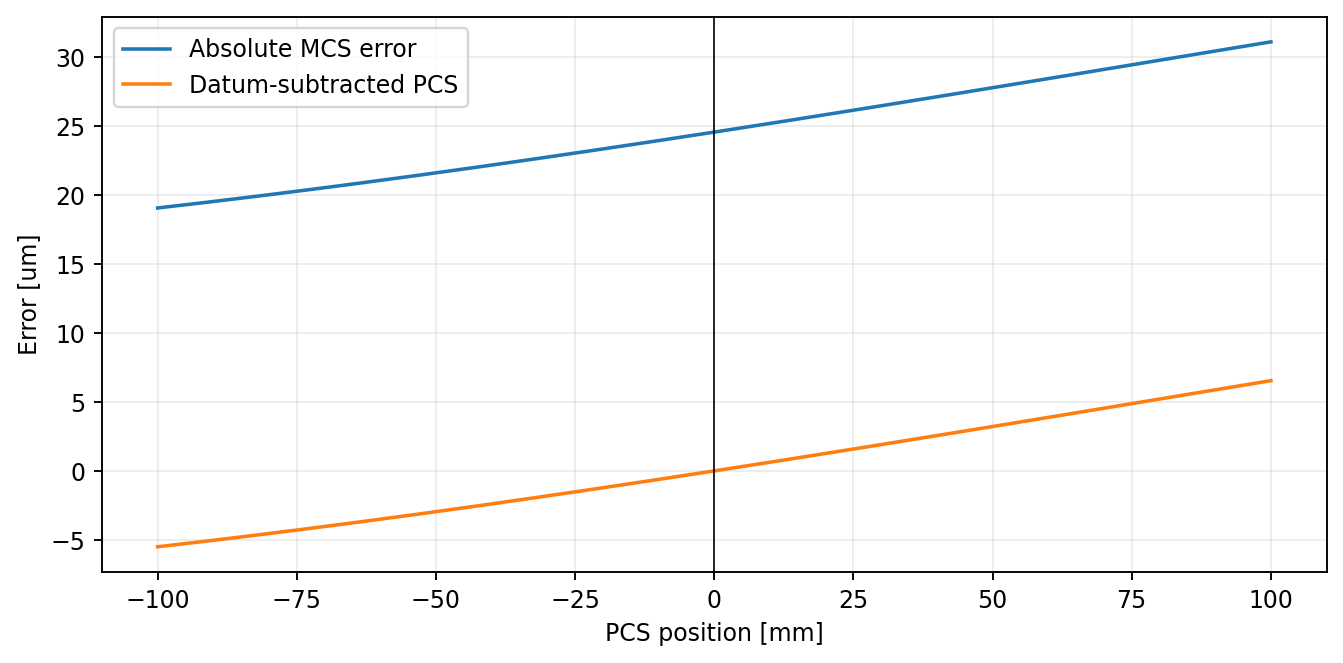
\includegraphics[width=.97\linewidth,height=73mm,keepaspectratio]{figures/pcs_mapping.png}\par\small\refstepcounter{figure}\textbf{Figure \thefigure.} Machine-coordinate and datum-relative part-coordinate maps.\end{center}

\begin{center}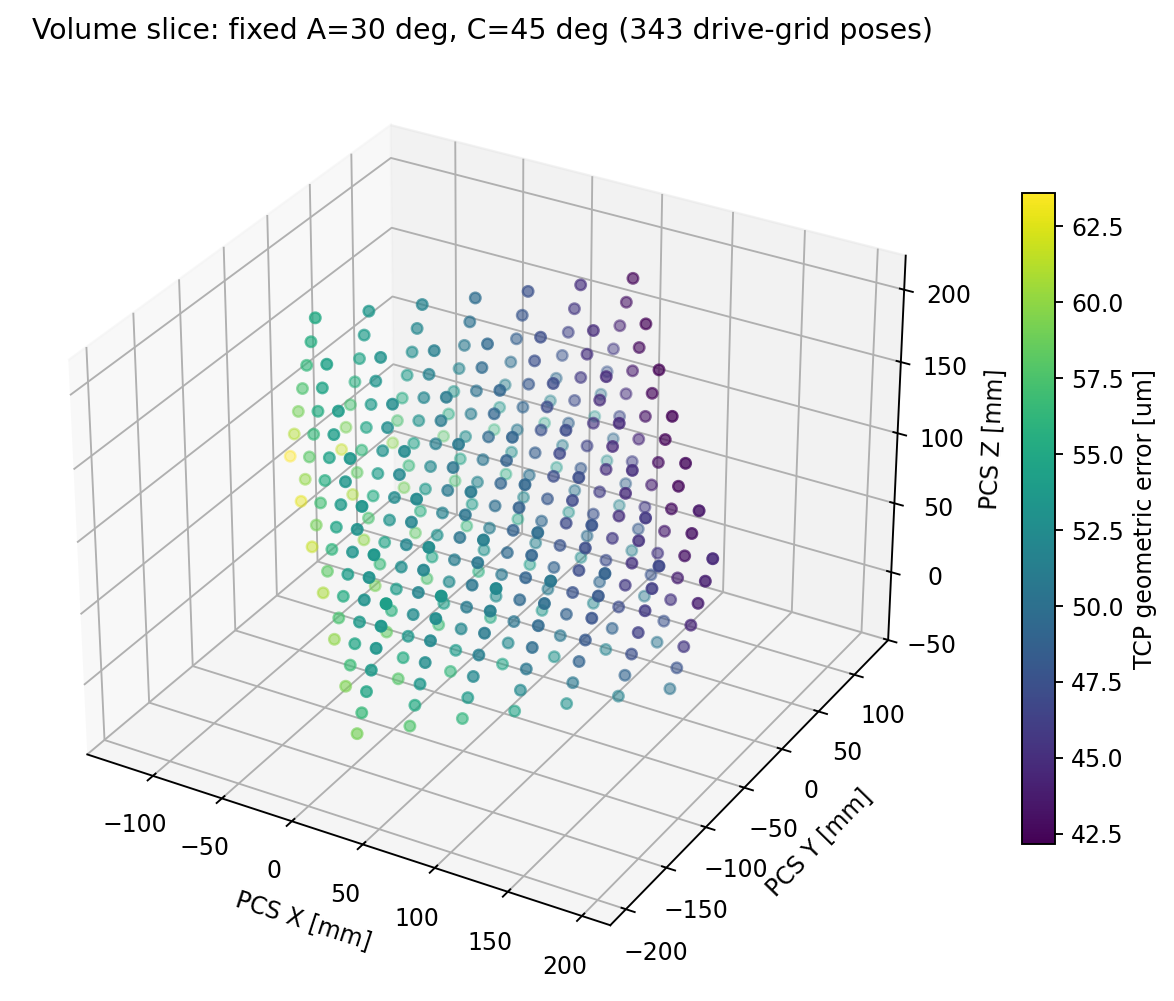
\includegraphics[width=.97\linewidth,height=73mm,keepaspectratio]{figures/volume_map.png}\par\small\refstepcounter{figure}\textbf{Figure \thefigure.} Spatial variation of TCP error at a fixed table orientation.\end{center}

\clearpage

\subsection{Sensitivity and inverse iteration}

The sensitivity sweep perturbs one geometric channel at a time and follows the same path. A small response may reflect the chosen path or the direction of the lever arm. With enlarged errors the maximum position residual drops from 1809.07 to 7.235 to 0.0167 micrometres over the first two updates. The convergence trace tests whether re-evaluating the geometry improves the command.

\par{\small\textit{Implementation}\quad \file{fiveaxis.py}\enspace /\enspace \file{experiments.py}}\par

\begin{center}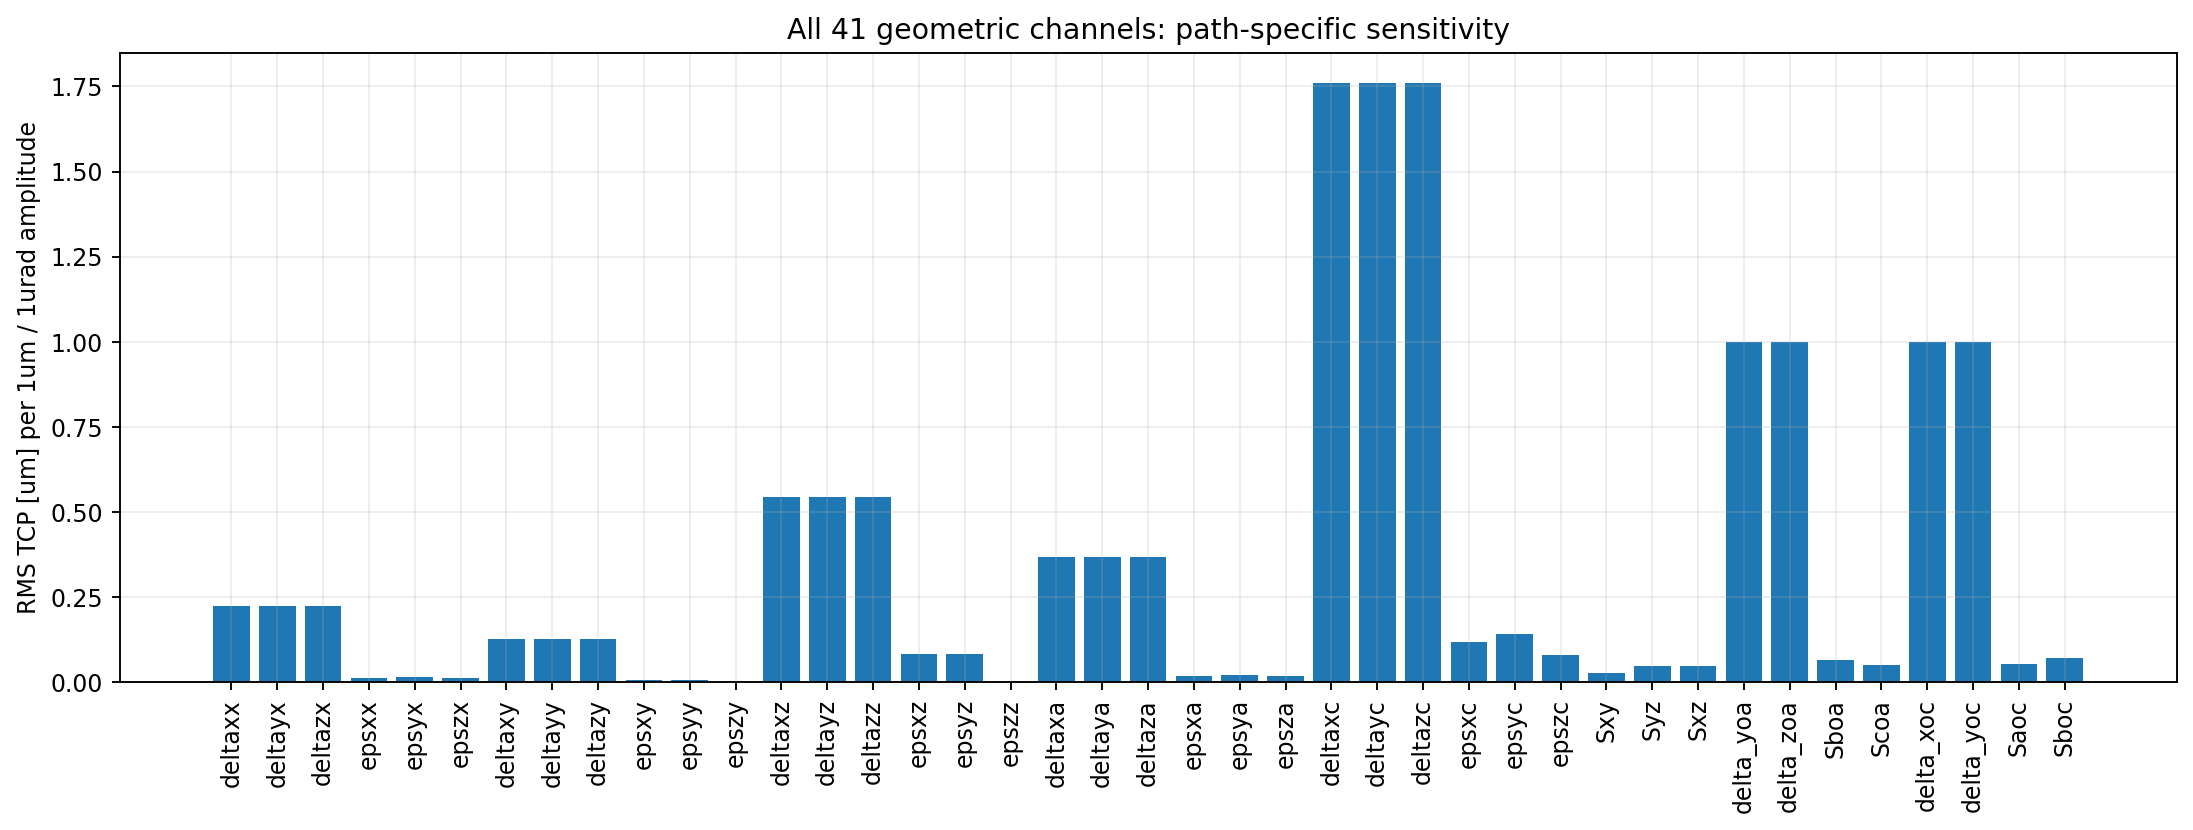
\includegraphics[width=.97\linewidth,height=73mm,keepaspectratio]{figures/sensitivity_41.png}\par\small\refstepcounter{figure}\textbf{Figure \thefigure.} Position response to each of the 30 motion-dependent and 11 fixed geometric channels.\end{center}

\begin{center}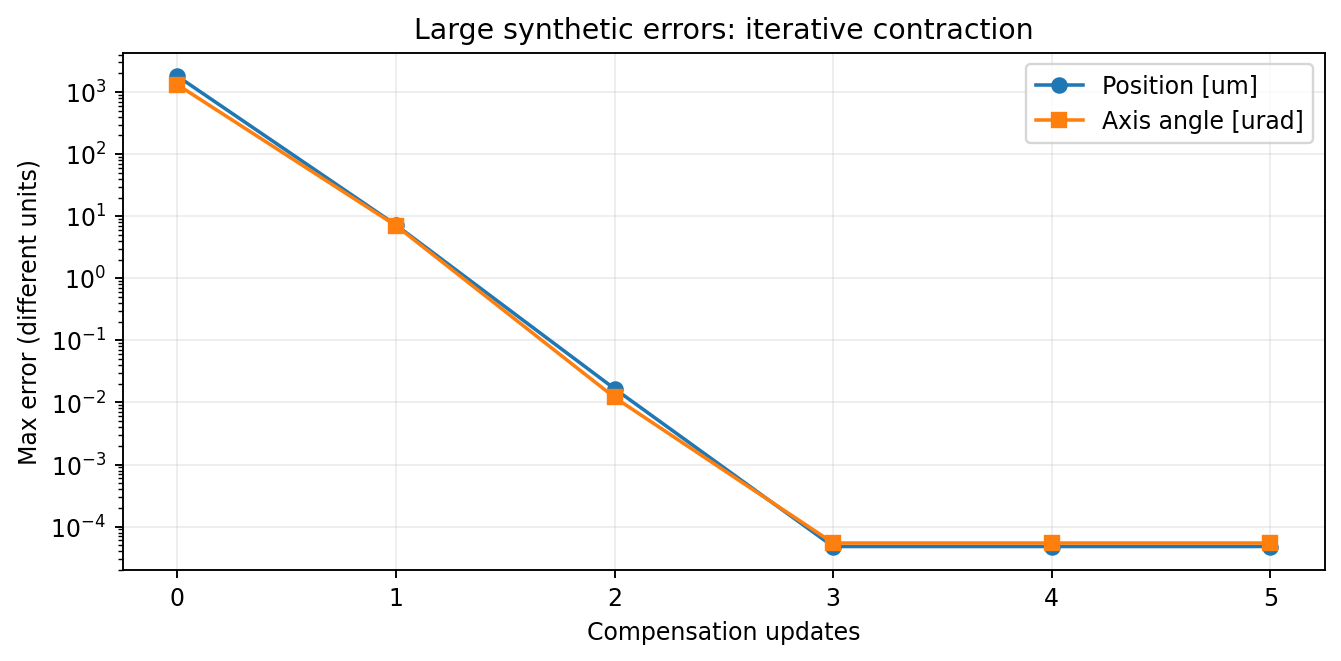
\includegraphics[width=.97\linewidth,height=73mm,keepaspectratio]{figures/iteration.png}\par\small\refstepcounter{figure}\textbf{Figure \thefigure.} Maximum residual versus compensation iteration in the enlarged-error test.\end{center}

\clearpage

\subsection{Fixture geometry and the rotary inverse}

Two readings at heights $H,H_1$ isolate A-axis tilt through $\epsilon_x=-(t_1-t_0)/(H_1-H)$, where $t$ is the tangential reading. A displaced radius $L$ supplies a second angular lever. In the noise-free implementation check, a true $+30$ microradian tilt returns $-30$ with the literal printed inverse; the corrected inverse recovers the input. The scaled condition number drops from 32,724 at 0.01 mm height separation to 5.66 at 100 mm.

\par{\small\textit{Implementation}\quad \file{calibration.py}\enspace /\enspace \file{tests/verify.py}}\par

\begin{center}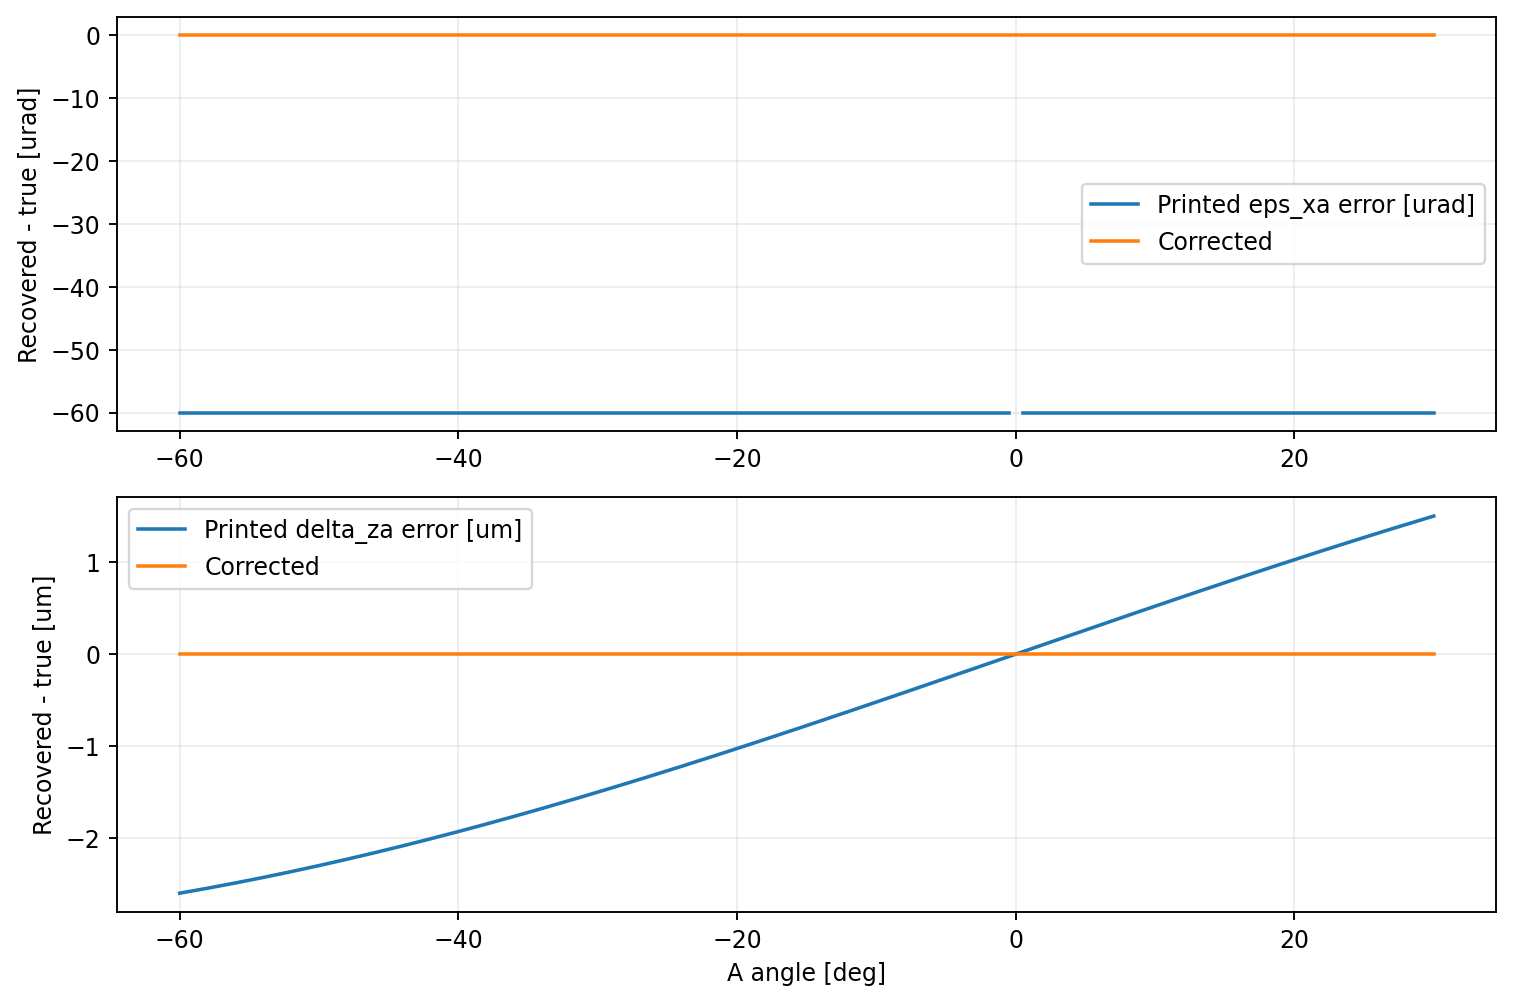
\includegraphics[width=.97\linewidth,height=73mm,keepaspectratio]{figures/eq29_audit.png}\par\small\refstepcounter{figure}\textbf{Figure \thefigure.} Literal and rederived inverses applied to measurements generated by the same forward equations.\end{center}

\begin{center}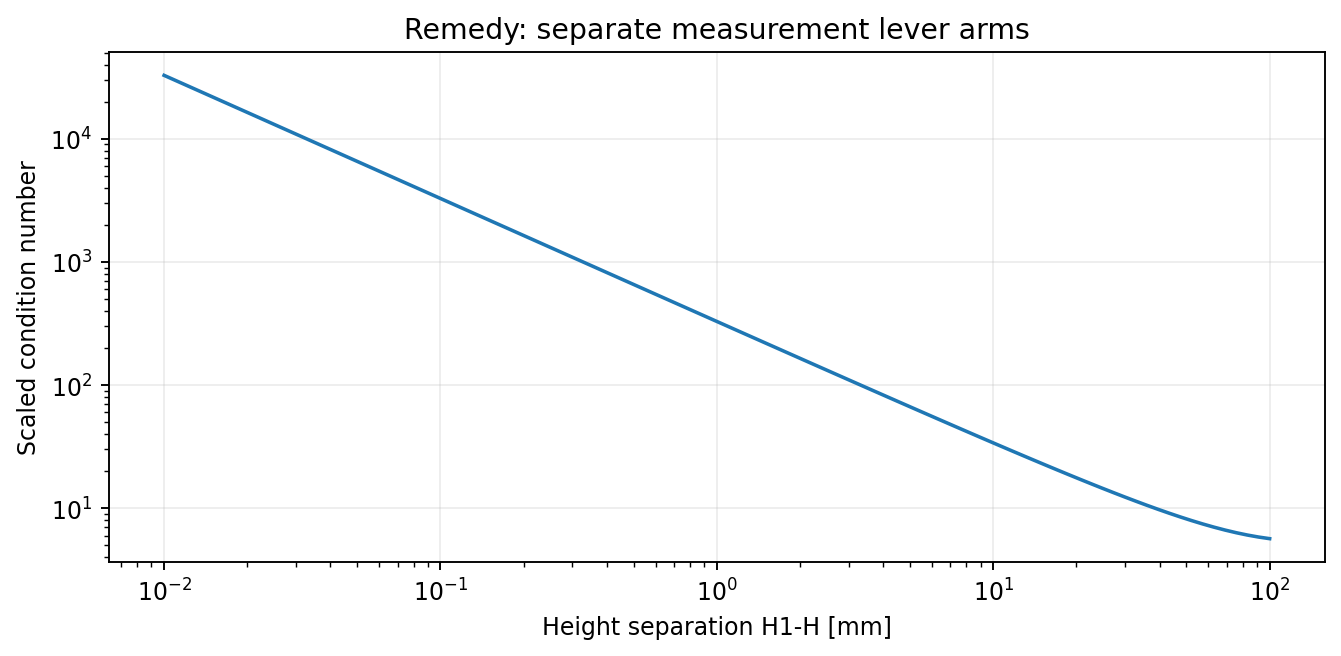
\includegraphics[width=.97\linewidth,height=73mm,keepaspectratio]{figures/calibration_geometry.png}\par\small\refstepcounter{figure}\textbf{Figure \thefigure.} Noise amplification is most severe as the two fixture heights coincide.\end{center}

\clearpage

\subsection{Identifying fixed and moving rotary errors}

Each row of the calibration matrix projects a displacement sensitivity along the ballbar direction. The full three-direction design resolves 44 of 44 parameters in this baseline. Radial readings alone resolve 40. The alternating fit cycles between fixed alignment and motion-dependent coefficients; residual convergence measures agreement with the measurements, while weak parameter directions can remain uncertain.

\par{\small\textit{Implementation}\quad \file{calibration.py}\enspace /\enspace \file{experiments.py}}\par

\begin{center}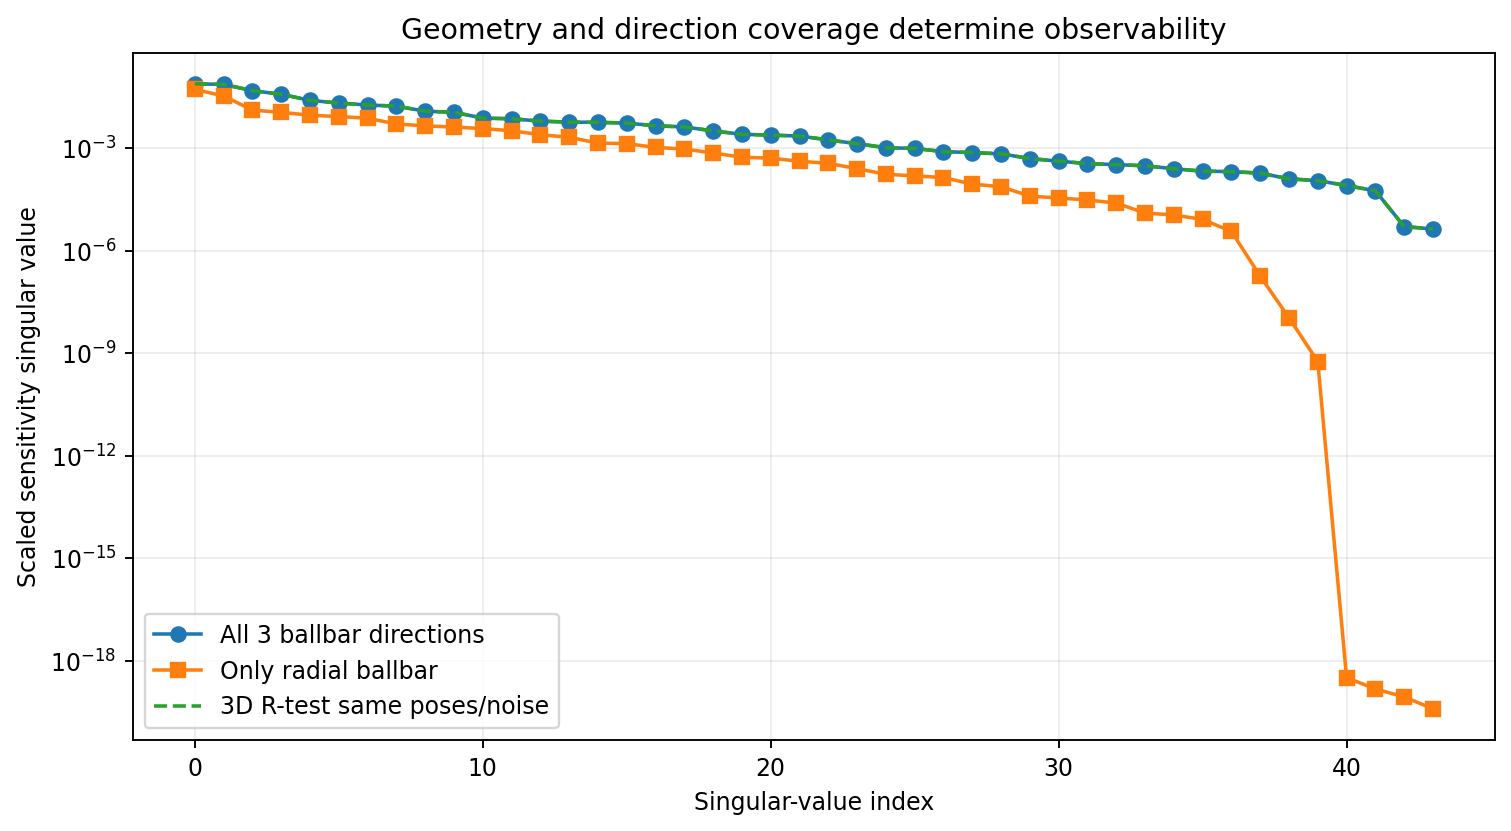
\includegraphics[width=.97\linewidth,height=73mm,keepaspectratio]{figures/observability.png}\par\small\refstepcounter{figure}\textbf{Figure \thefigure.} Singular spectra for complete, radial-only and Cartesian observation systems.\end{center}

\begin{center}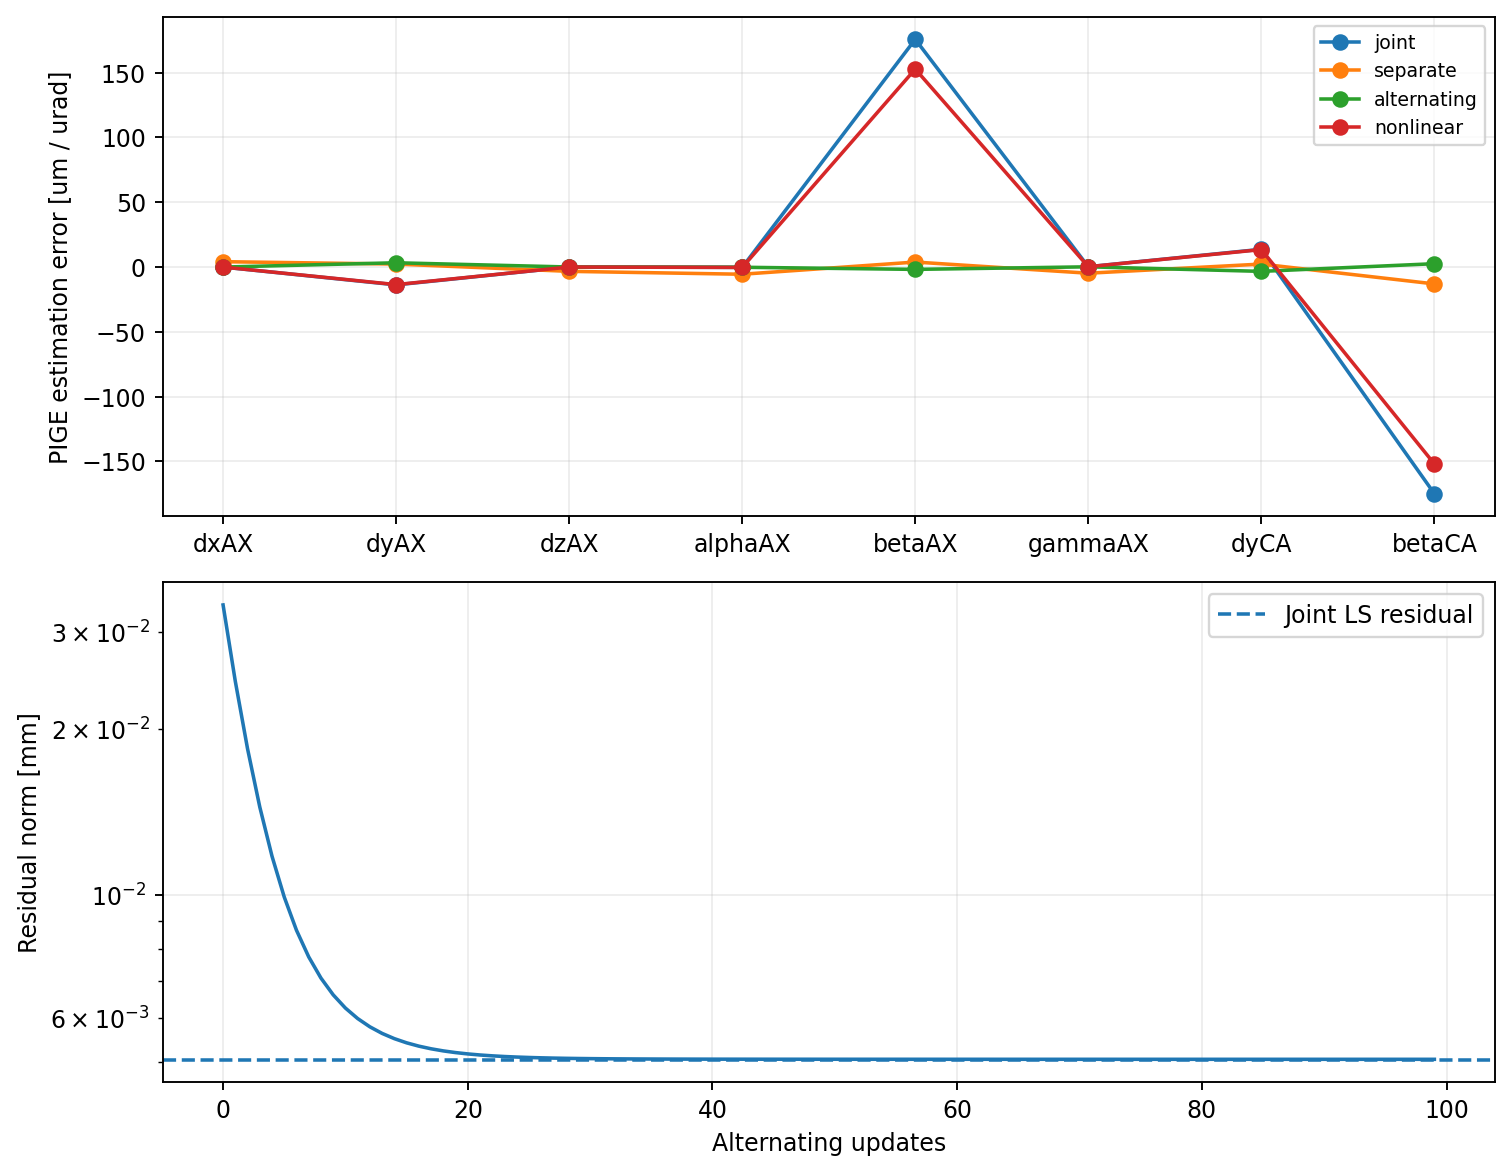
\includegraphics[width=.97\linewidth,height=73mm,keepaspectratio]{figures/pige_decoupling.png}\par\small\refstepcounter{figure}\textbf{Figure \thefigure.} Fixed alignment estimates and residual history during alternating fits.\end{center}

\clearpage

\subsection{What the fitted rotary maps look like}

The figures compare the six components per rotary axis. On held-out sensor readings, joint, alternating and nonlinear fits give RMS errors of 0.0582, 0.0575 and 0.0550 micrometres, respectively. Their normalized parameter RMSEs are 8.60, 1.30 and 7.89. Similar predicted sensor traces can arise from substantially different coefficients.

\par{\small\textit{Implementation}\quad \file{calibration.py}\enspace /\enspace \file{experiments.py}}\par

\begin{center}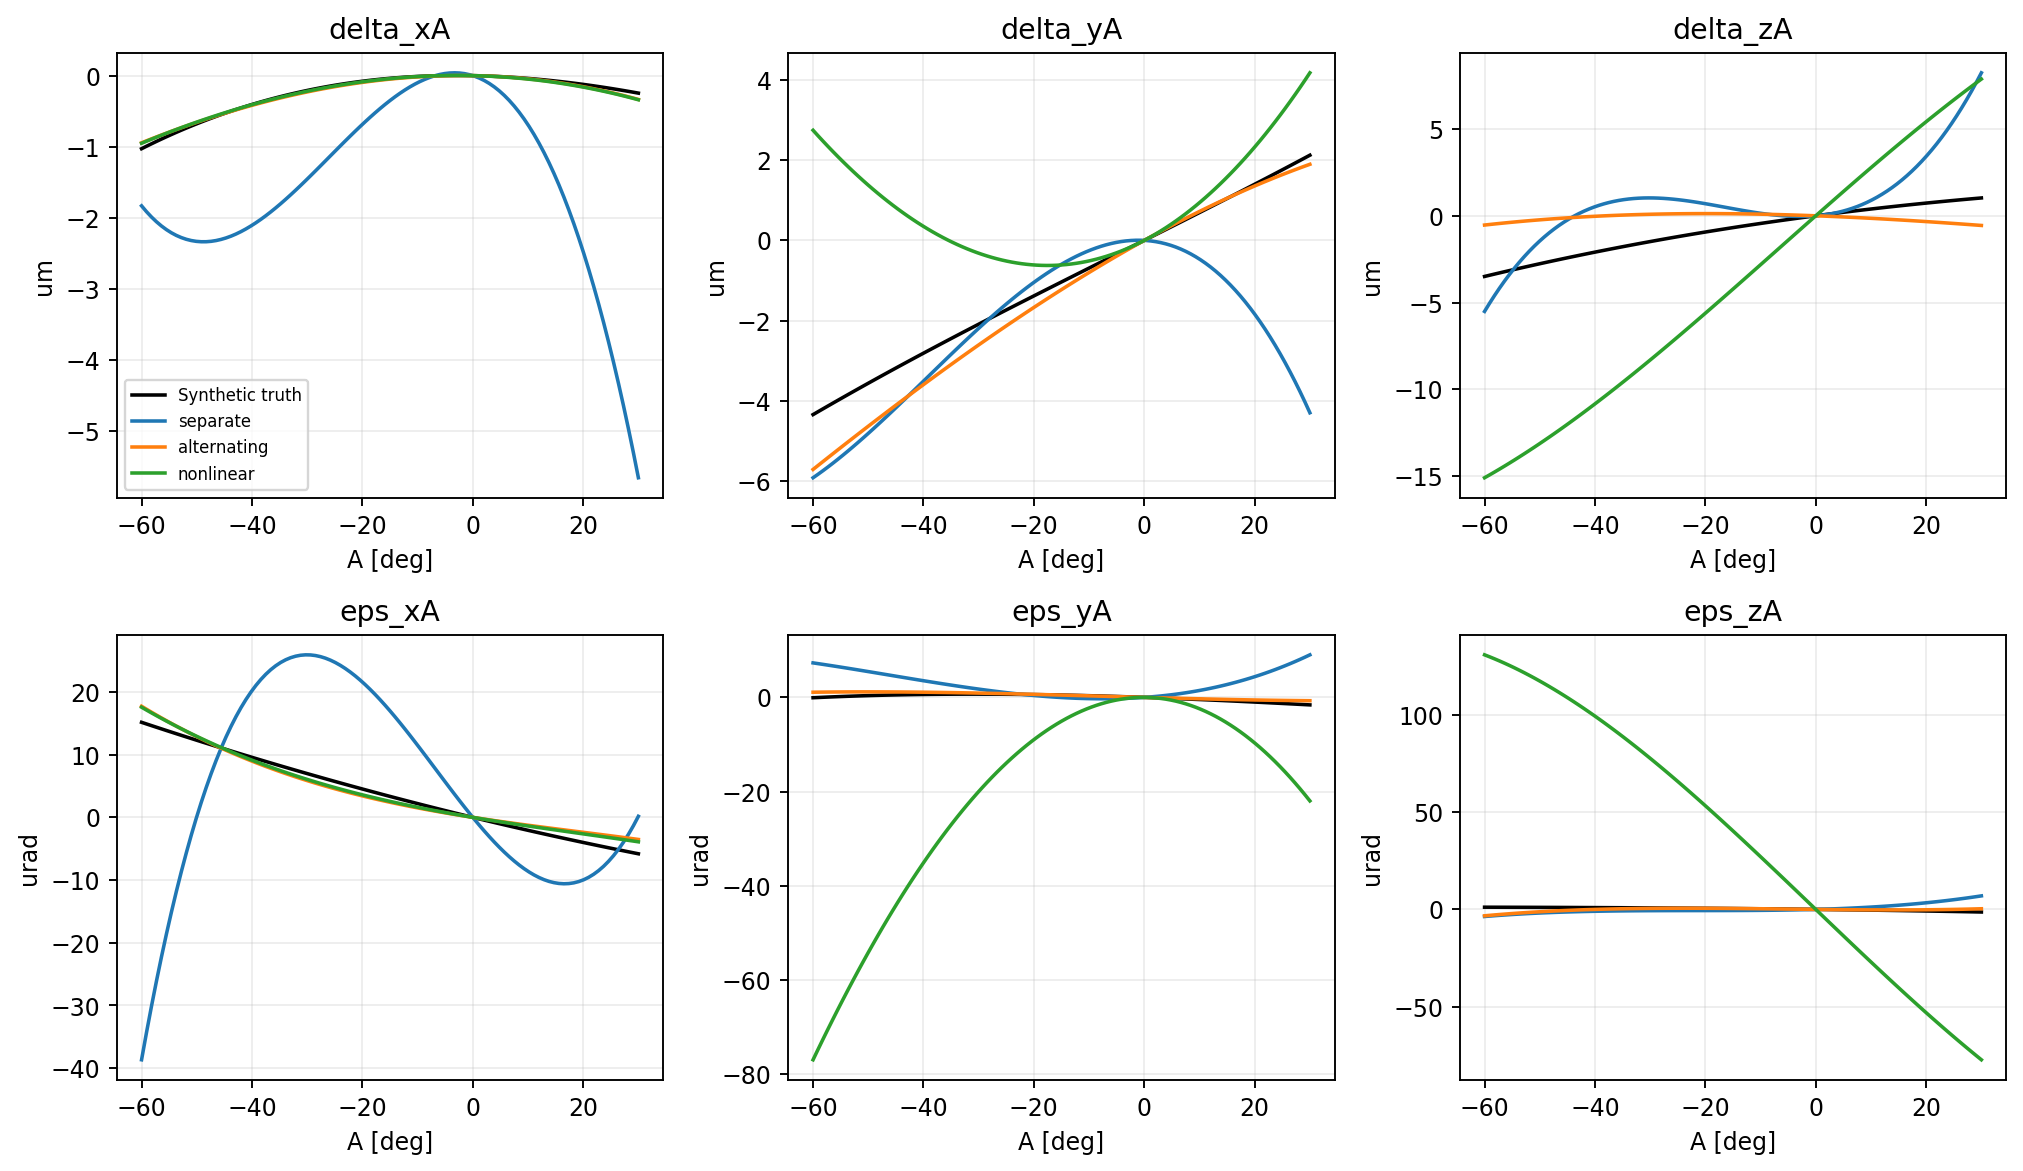
\includegraphics[width=.97\linewidth,height=73mm,keepaspectratio]{figures/rotary_pdge_A.png}\par\small\refstepcounter{figure}\textbf{Figure \thefigure.} A-axis displacement and angular maps estimated from the virtual measurements.\end{center}

\begin{center}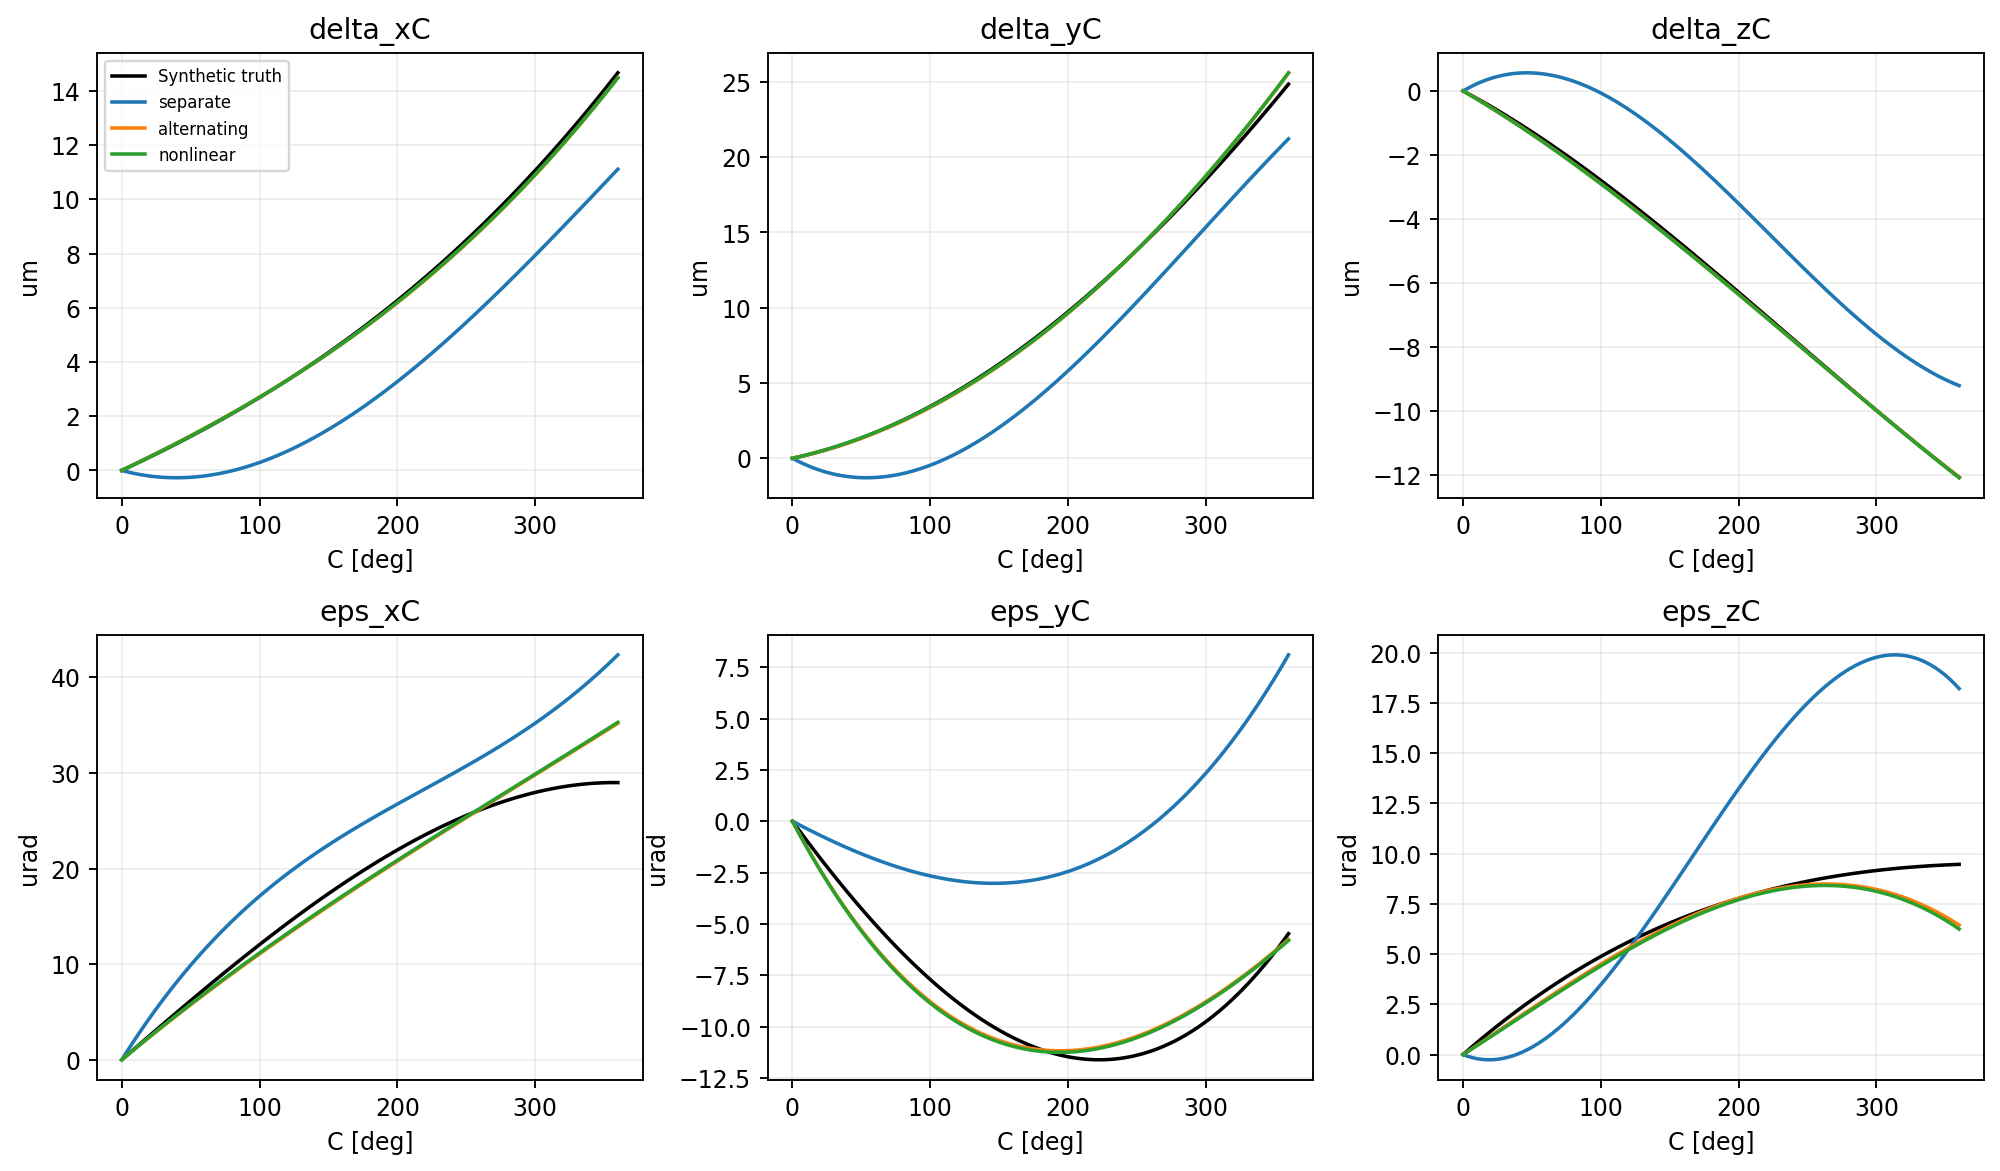
\includegraphics[width=.97\linewidth,height=73mm,keepaspectratio]{figures/rotary_pdge_C.png}\par\small\refstepcounter{figure}\textbf{Figure \thefigure.} C-axis maps from the same four estimation strategies.\end{center}

\clearpage

\subsection{Estimating the linear-axis maps}

Fitting noisy component measurements replaces the ideal exact-map control. The fitted model gives 0.861 micrometres TCP RMS on its test path. Dropping the three linear-axis roll channels raises that value to 0.929. Roll couples to position through offsets, so an angular channel with little effect in one setup can matter at another tool length or pose.

\par{\small\textit{Implementation}\quad \file{experiments.py}\enspace /\enspace \file{calibration.py}}\par

\begin{center}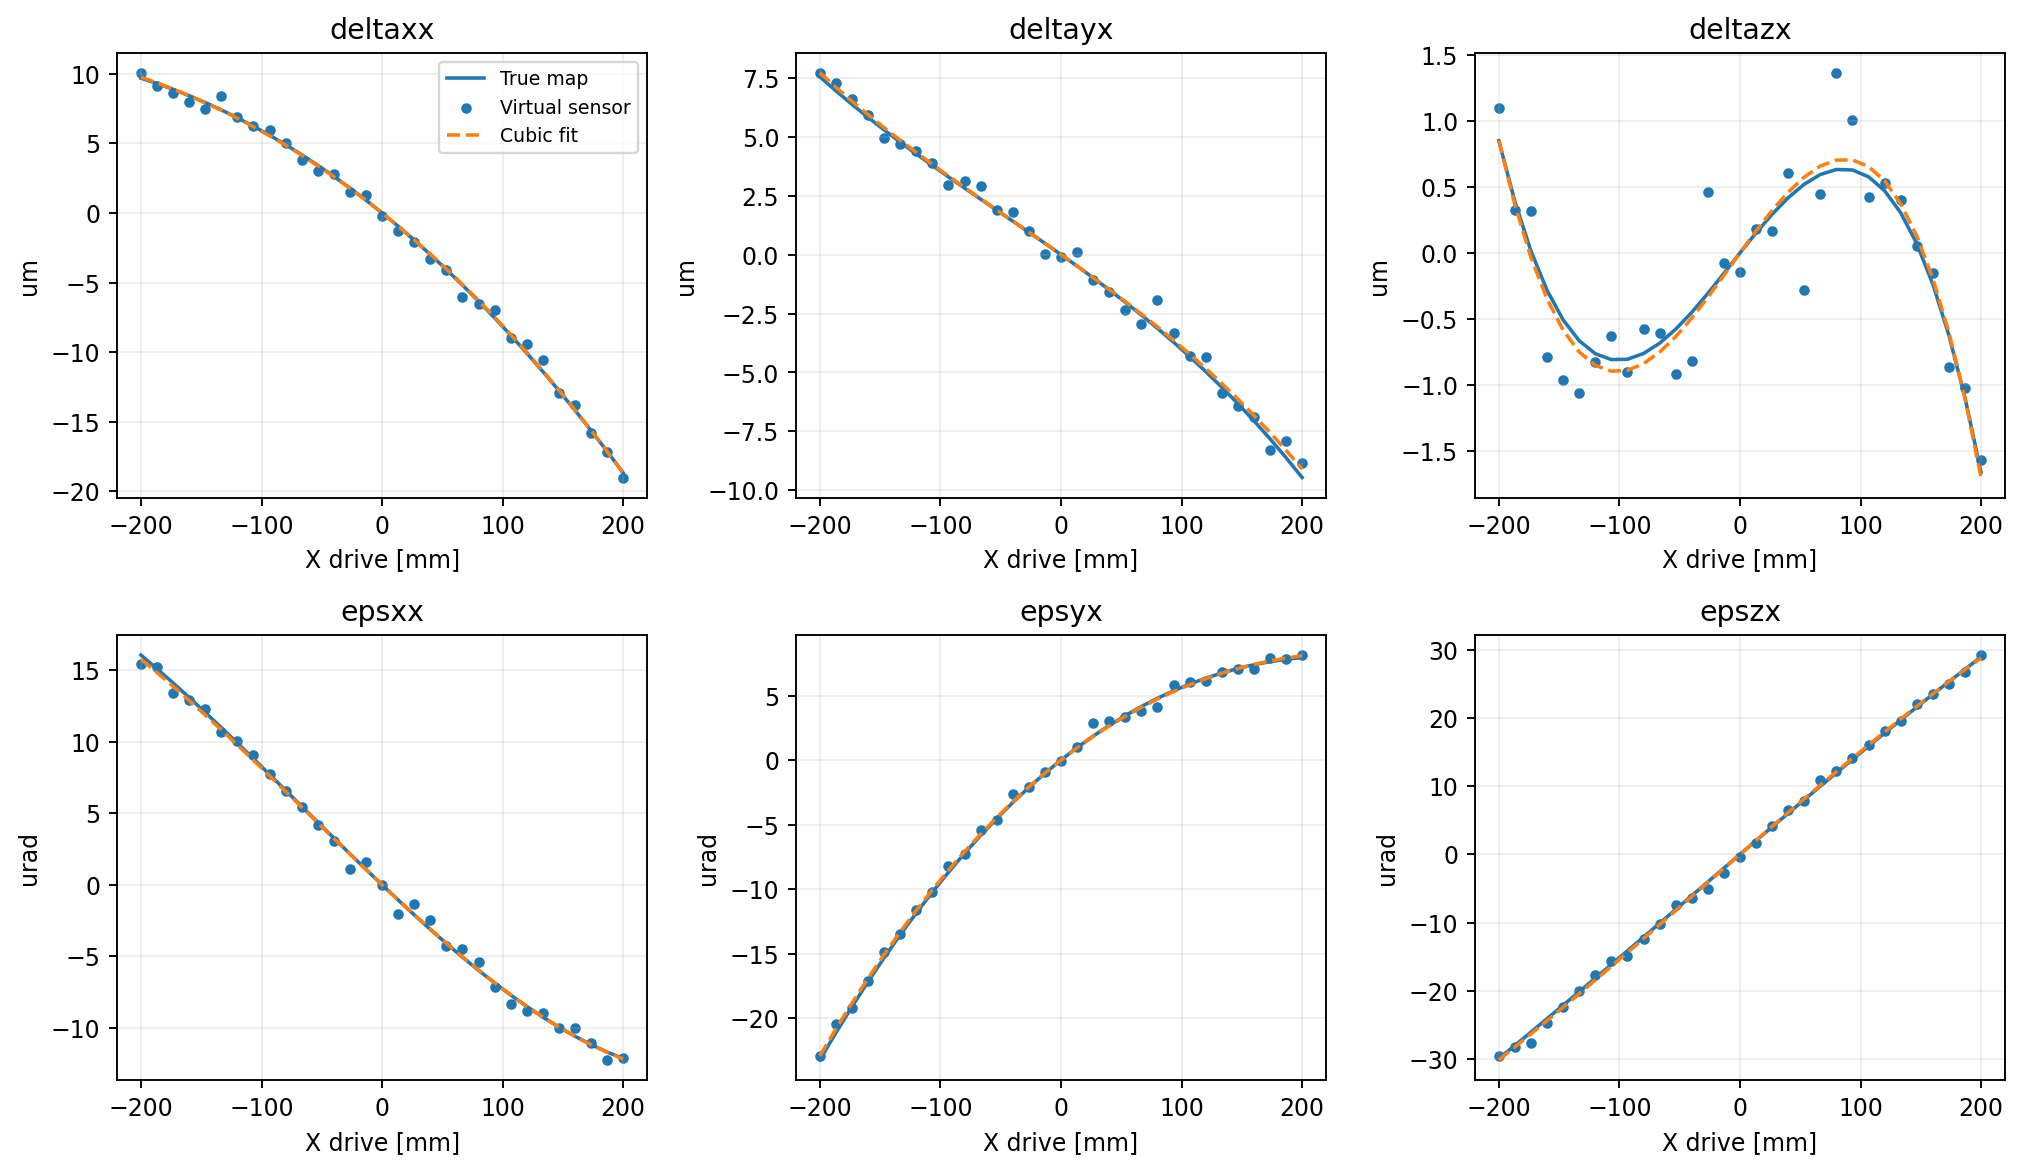
\includegraphics[width=.97\linewidth,height=73mm,keepaspectratio]{figures/linear_sensors.png}\par\small\refstepcounter{figure}\textbf{Figure \thefigure.} Six X-axis component observations, synthetic truth and fitted cubics.\end{center}

\begin{center}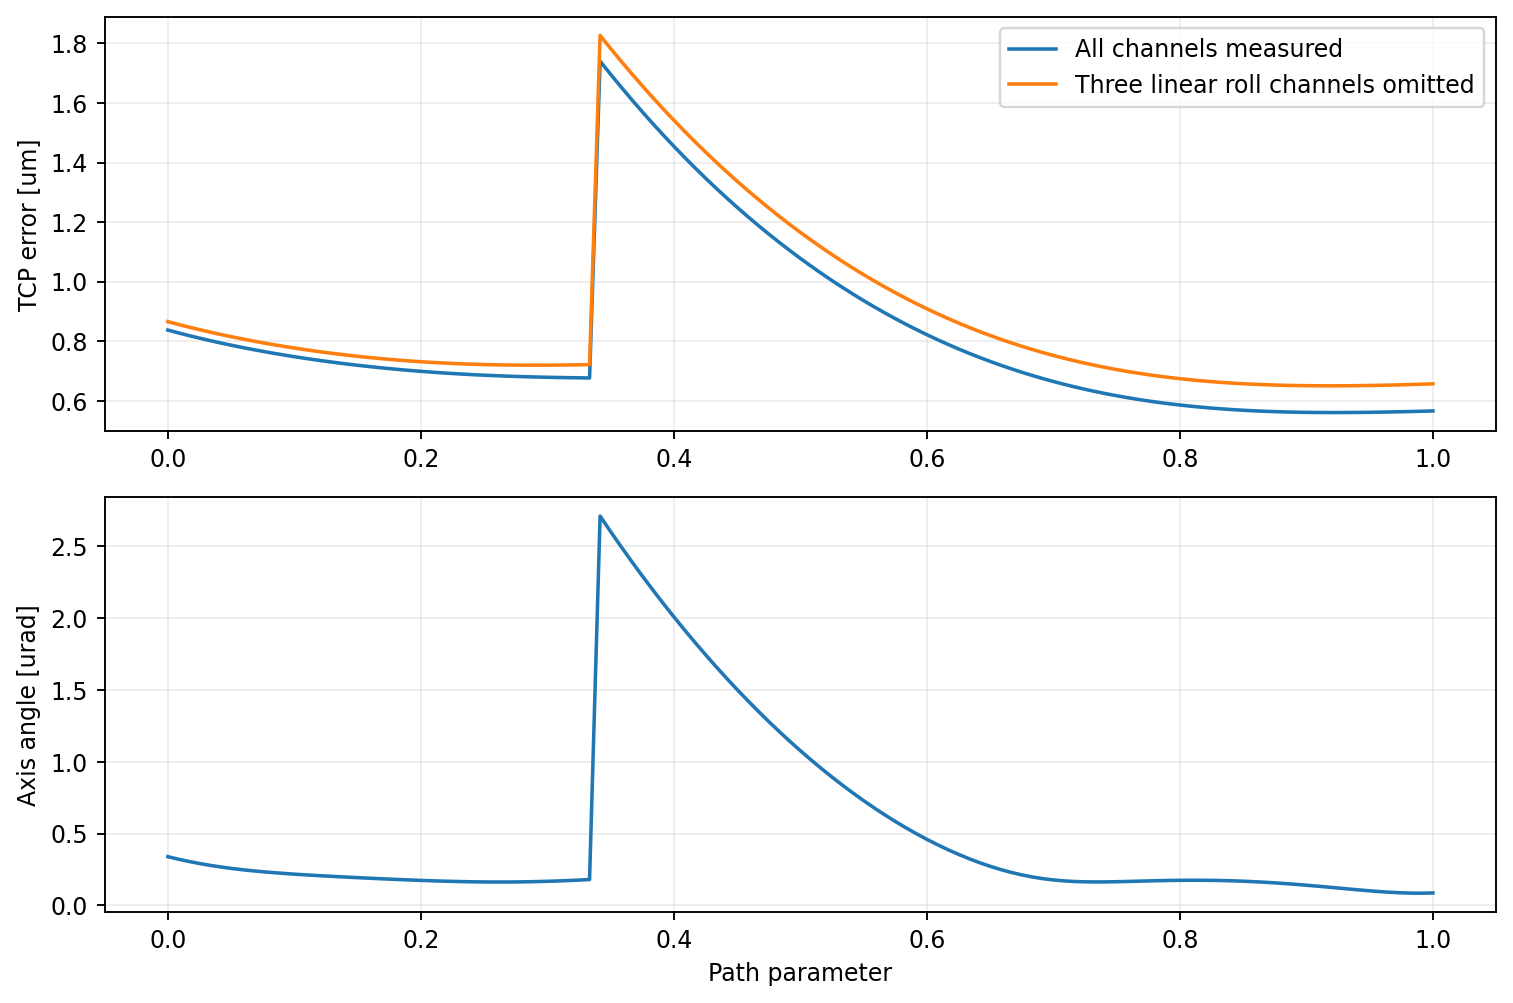
\includegraphics[width=.97\linewidth,height=73mm,keepaspectratio]{figures/roll_and_map_noise.png}\par\small\refstepcounter{figure}\textbf{Figure \thefigure.} Residuals using all fitted channels and after omitting linear-axis rolls.\end{center}

\clearpage

\subsection{Closing the loop from measurement to motion}

The model estimated from optical and ballbar data is applied to a different trajectory. TCP RMS falls from 92.442 to 0.546 micrometres and axis RMS from 58.483 to 7.823 microradians. Ballbar traces below provide a second view: a probe observes a projection of the geometric change and adds measurement noise. A small axial ballbar signal alone cannot certify the vector TCP error.

\par{\small\textit{Implementation}\quad \file{experiments.py}\enspace /\enspace \file{io_tools.py}}\par

\begin{center}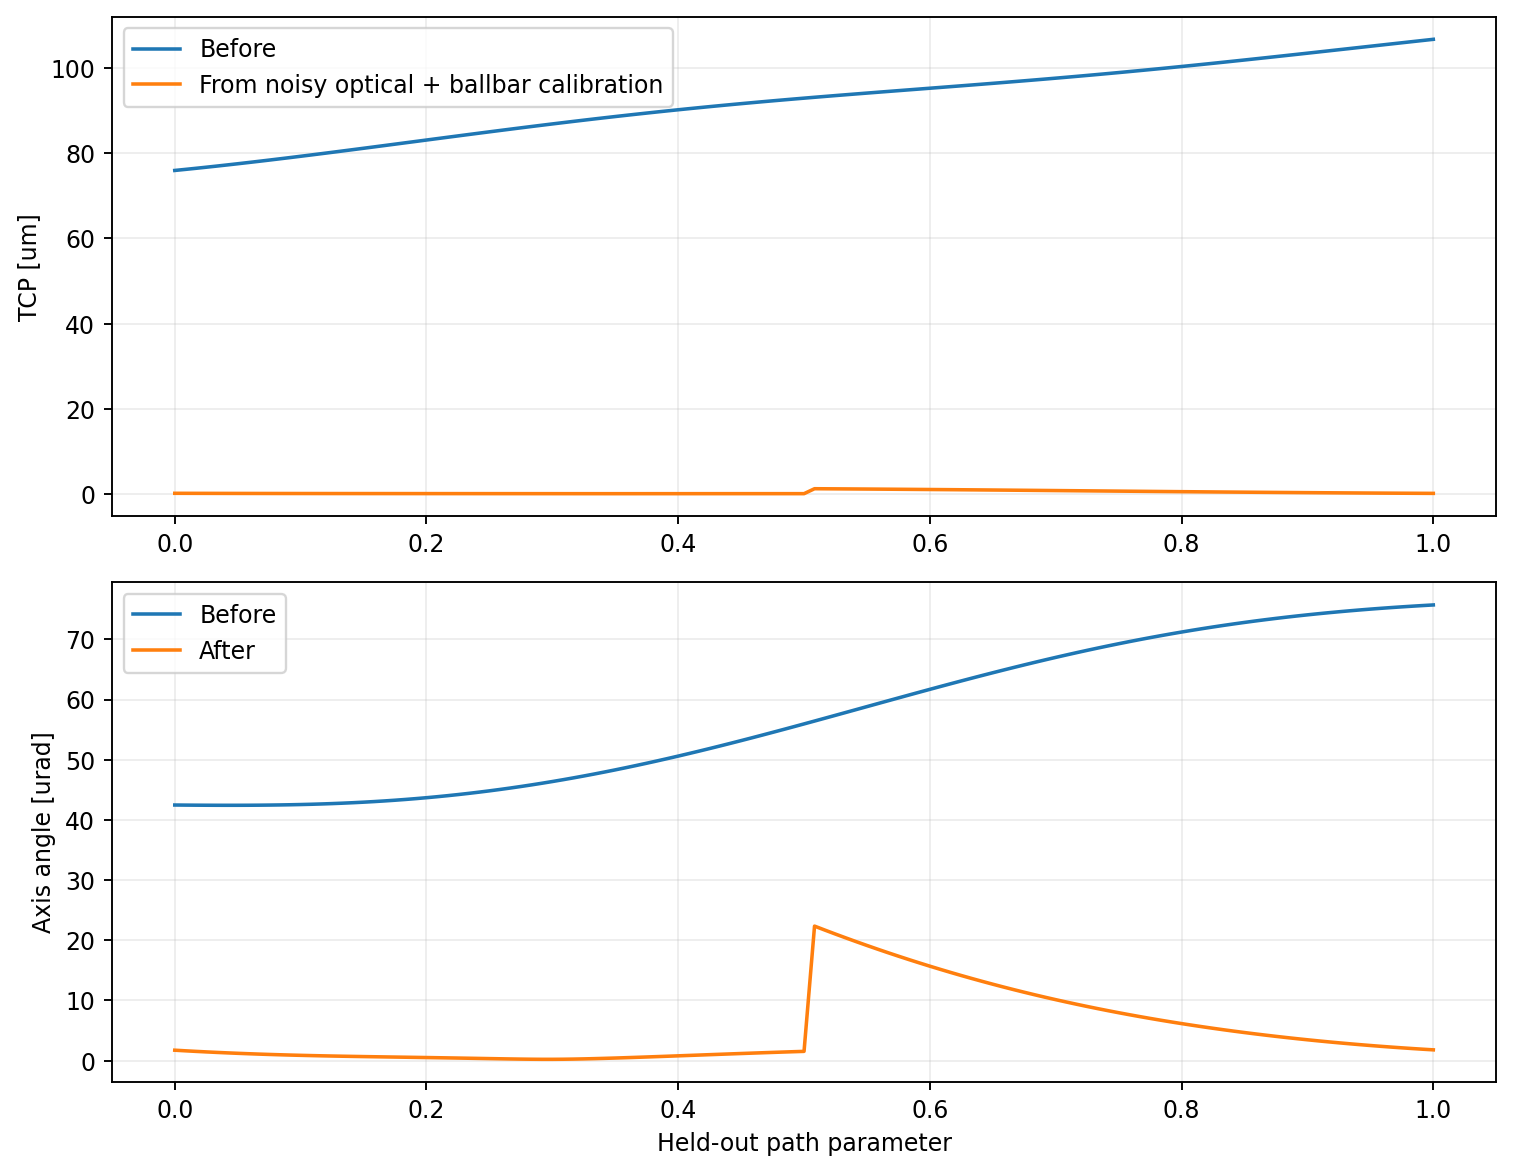
\includegraphics[width=.97\linewidth,height=73mm,keepaspectratio]{figures/calibration_to_compensation.png}\par\small\refstepcounter{figure}\textbf{Figure \thefigure.} Held-out TCP and orientation residuals before and after fitting the machine.\end{center}

\begin{center}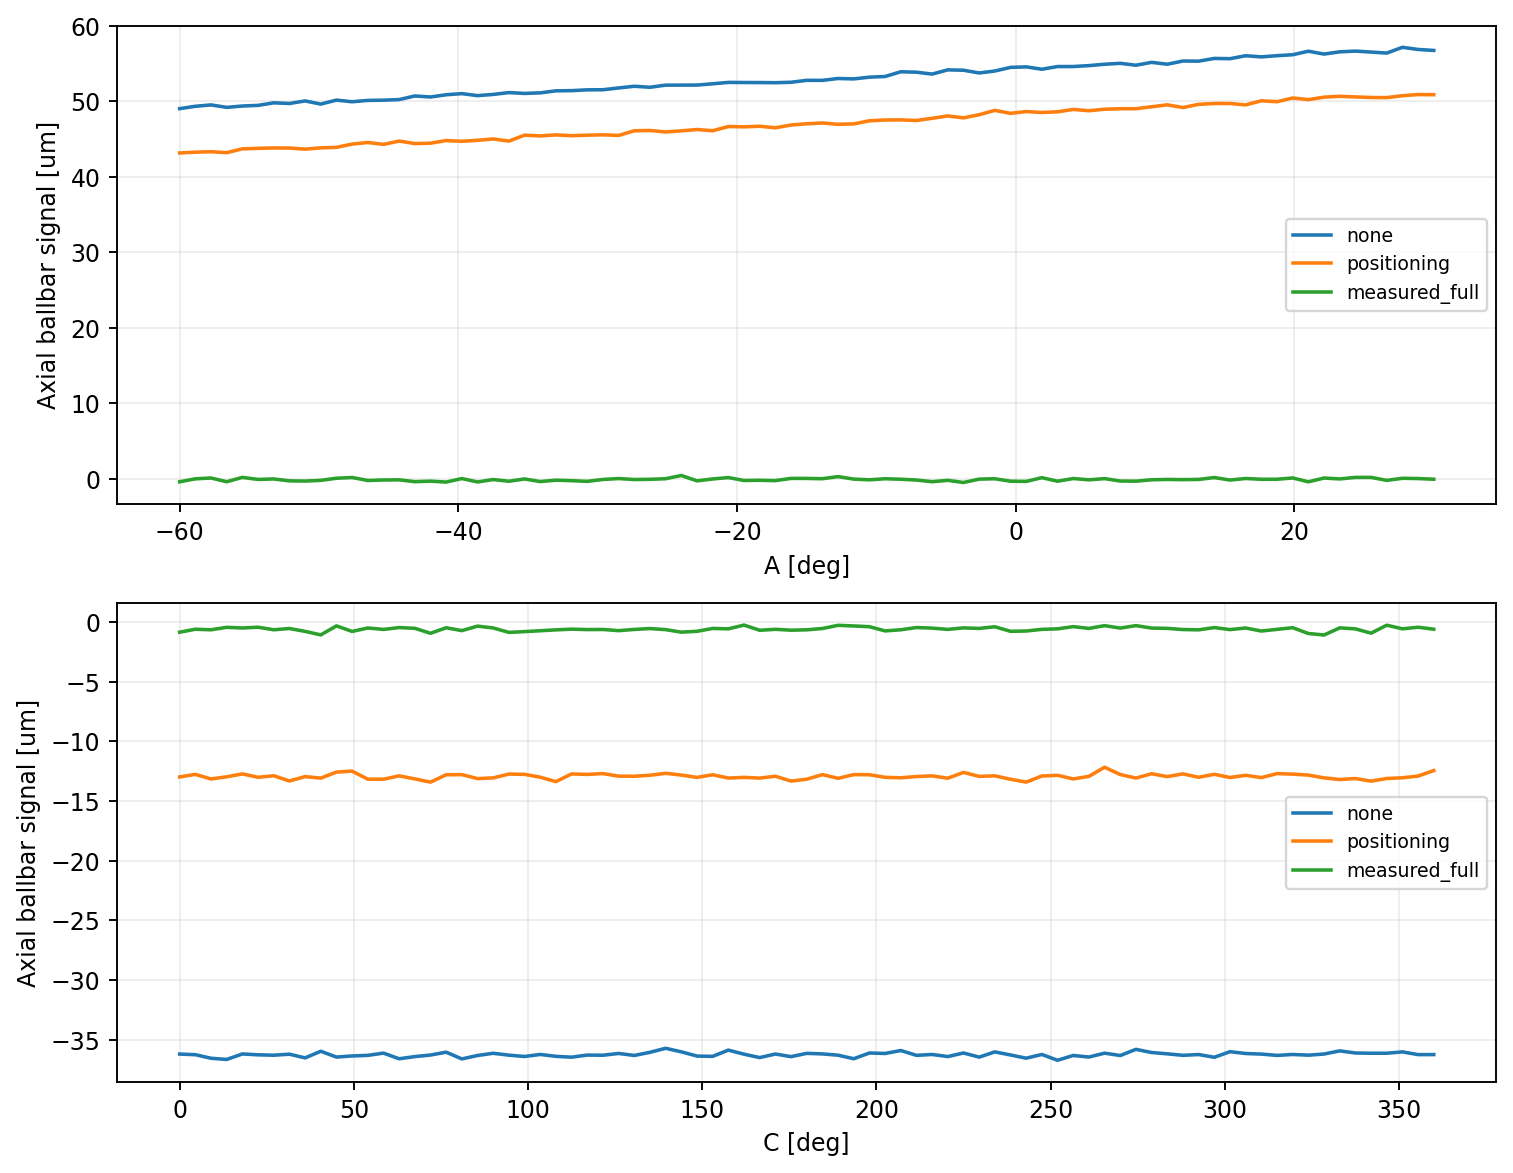
\includegraphics[width=.97\linewidth,height=73mm,keepaspectratio]{figures/ballbar_compensation.png}\par\small\refstepcounter{figure}\textbf{Figure \thefigure.} Virtual axial ballbar measurements before and after correction.\end{center}

\clearpage

\subsection{When a calibration becomes ill-conditioned}

The baseline coefficient-standard-deviation vector differs by 1.37\% from its 100-trial linear-noise prediction. That check concerns a specified calibration design. A separate singularity arises in the inverse motion: when the tool approaches the C-axis direction, azimuth becomes poorly determined. The scaled task-Jacobian condition rises from 2.79 at $60^\circ$ tilt to roughly 448,000 at $0.001^\circ$. Branch continuity helps choose commands across this region.

\par{\small\textit{Implementation}\quad \file{experiments.py}\enspace /\enspace \file{fiveaxis.py}}\par

\begin{center}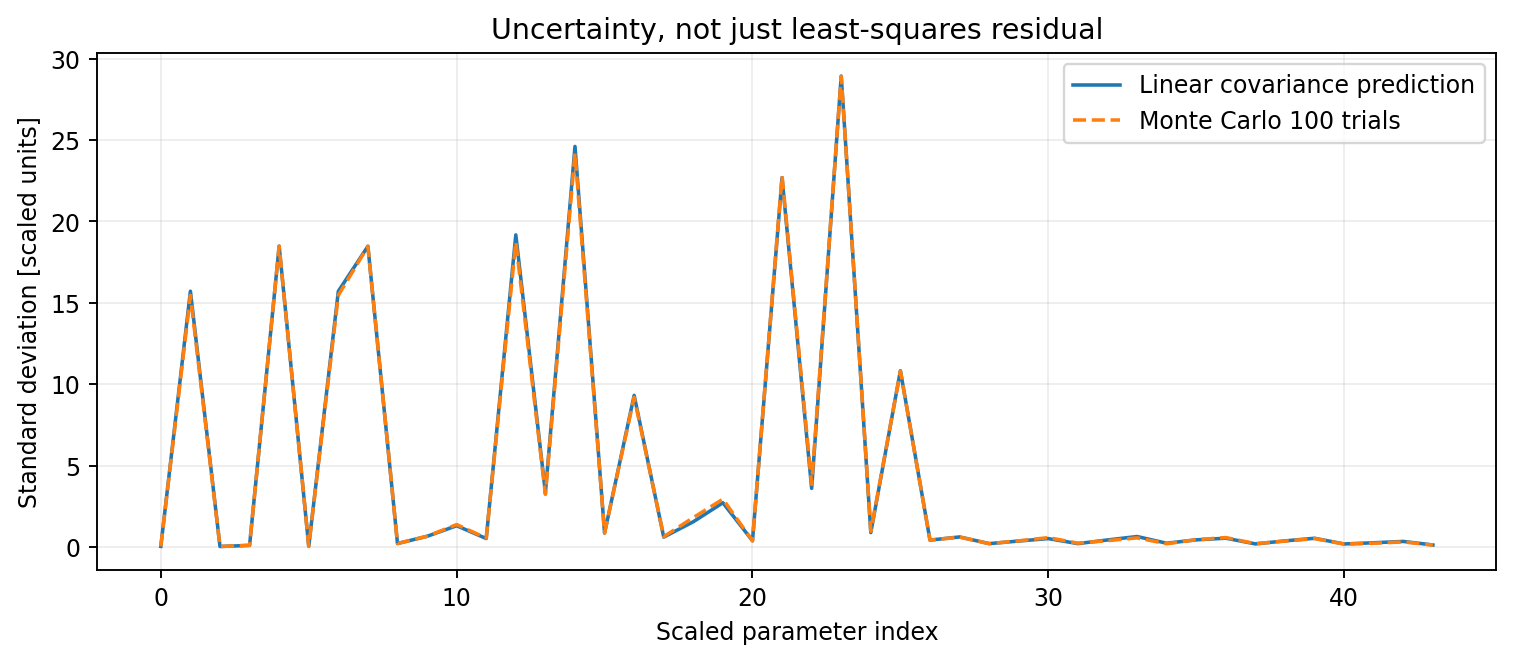
\includegraphics[width=.97\linewidth,height=73mm,keepaspectratio]{figures/uncertainty.png}\par\small\refstepcounter{figure}\textbf{Figure \thefigure.} Analytic parameter standard deviations and repeated calibration estimates.\end{center}

\begin{center}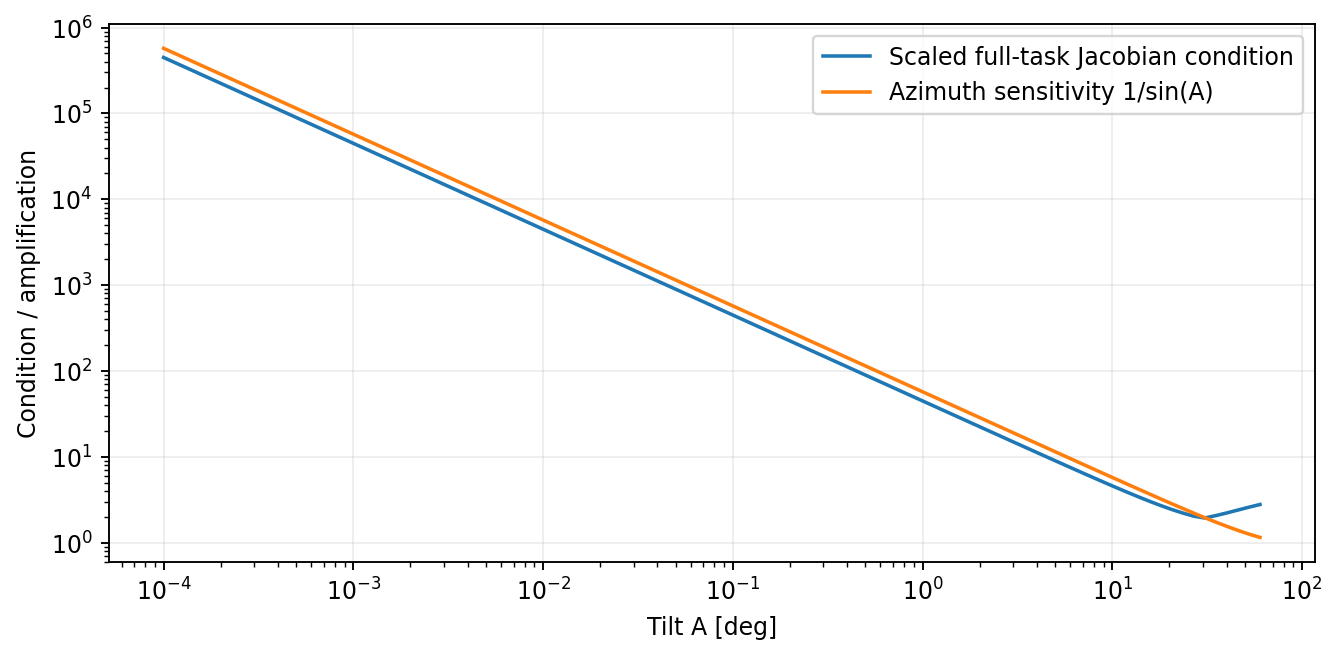
\includegraphics[width=.97\linewidth,height=73mm,keepaspectratio]{figures/singularity.png}\par\small\refstepcounter{figure}\textbf{Figure \thefigure.} Task-Jacobian conditioning and azimuth amplification near zero tilt.\end{center}

\clearpage

\section{Sensor errors, rotary representation and experimental design}

\subsection{Temperature drift and reversal play}

A fitted temperature-to-displacement map reduces pooled displacement RMS from 10.414 to 0.410 micrometres on the standalone thermal holdout. A separately identified play width of 23.993 micrometres reduces reversal-error RMS from 11.947 to 0.399. Temperature compensation uses an observed environmental state; play compensation requires the preceding direction and drive state.

\par{\small\textit{Implementation}\quad \file{remedies.py}\enspace /\enspace \file{experiments.py}}\par

\begin{center}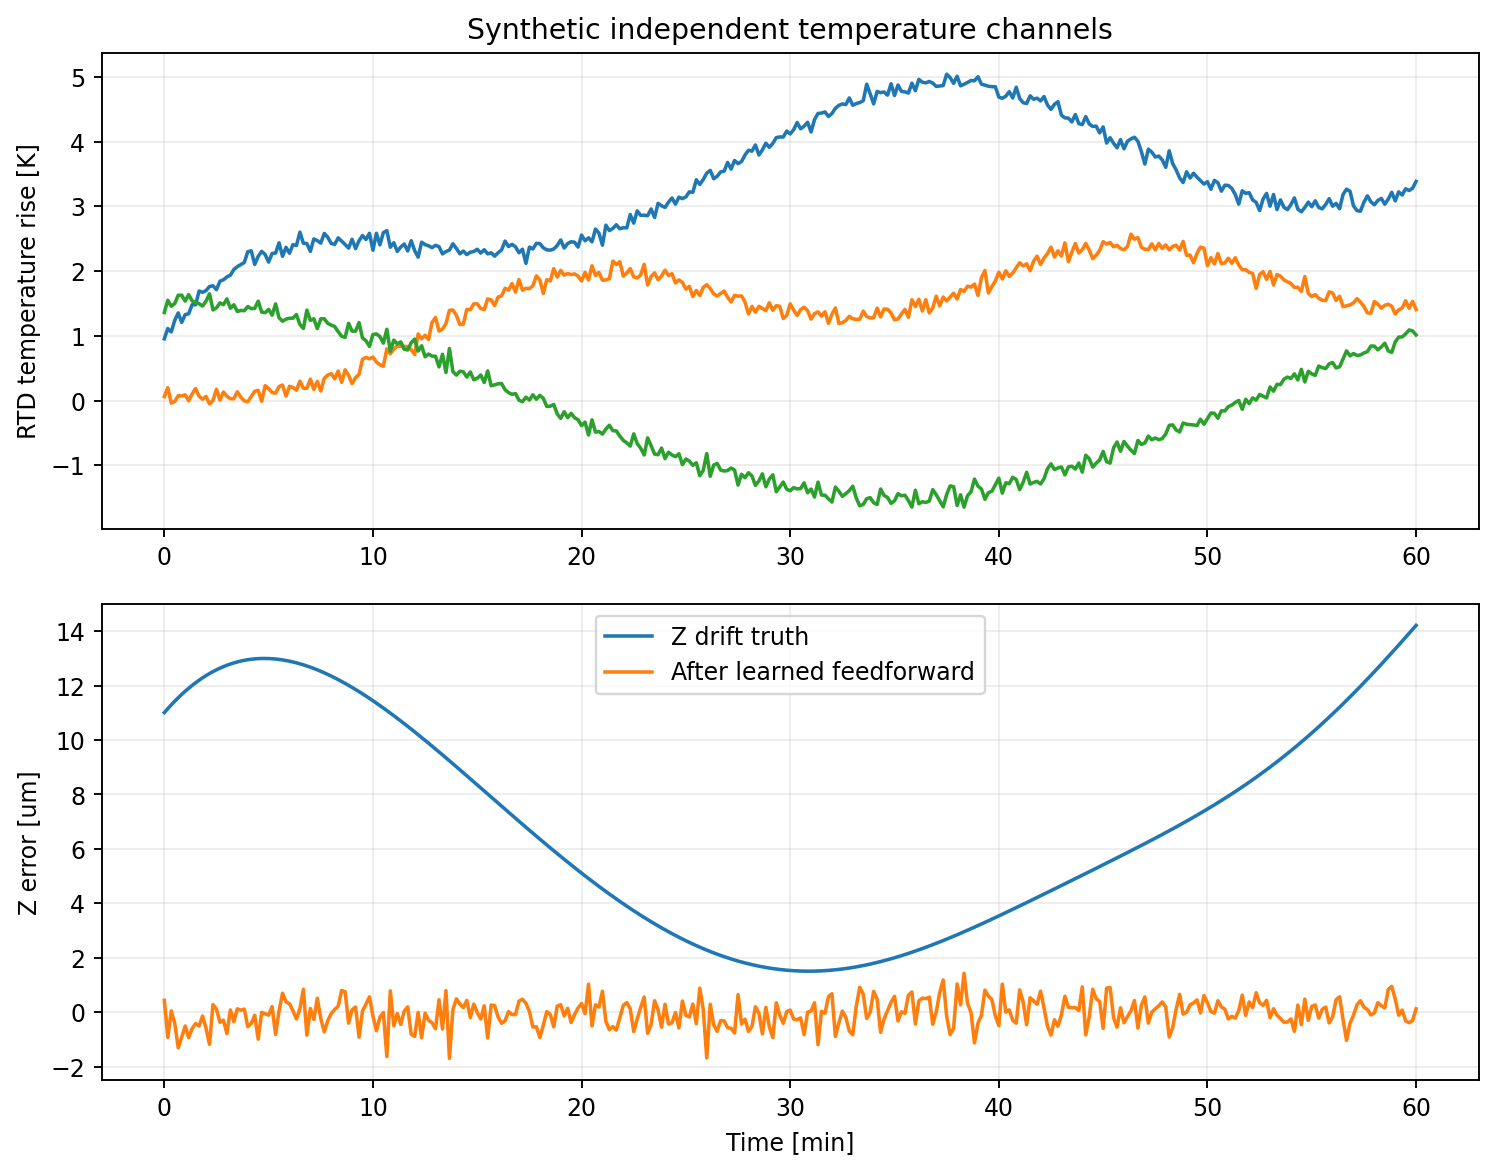
\includegraphics[width=.97\linewidth,height=73mm,keepaspectratio]{figures/thermal.png}\par\small\refstepcounter{figure}\textbf{Figure \thefigure.} Independent heating-cycle measurements and residual displacement.\end{center}

\begin{center}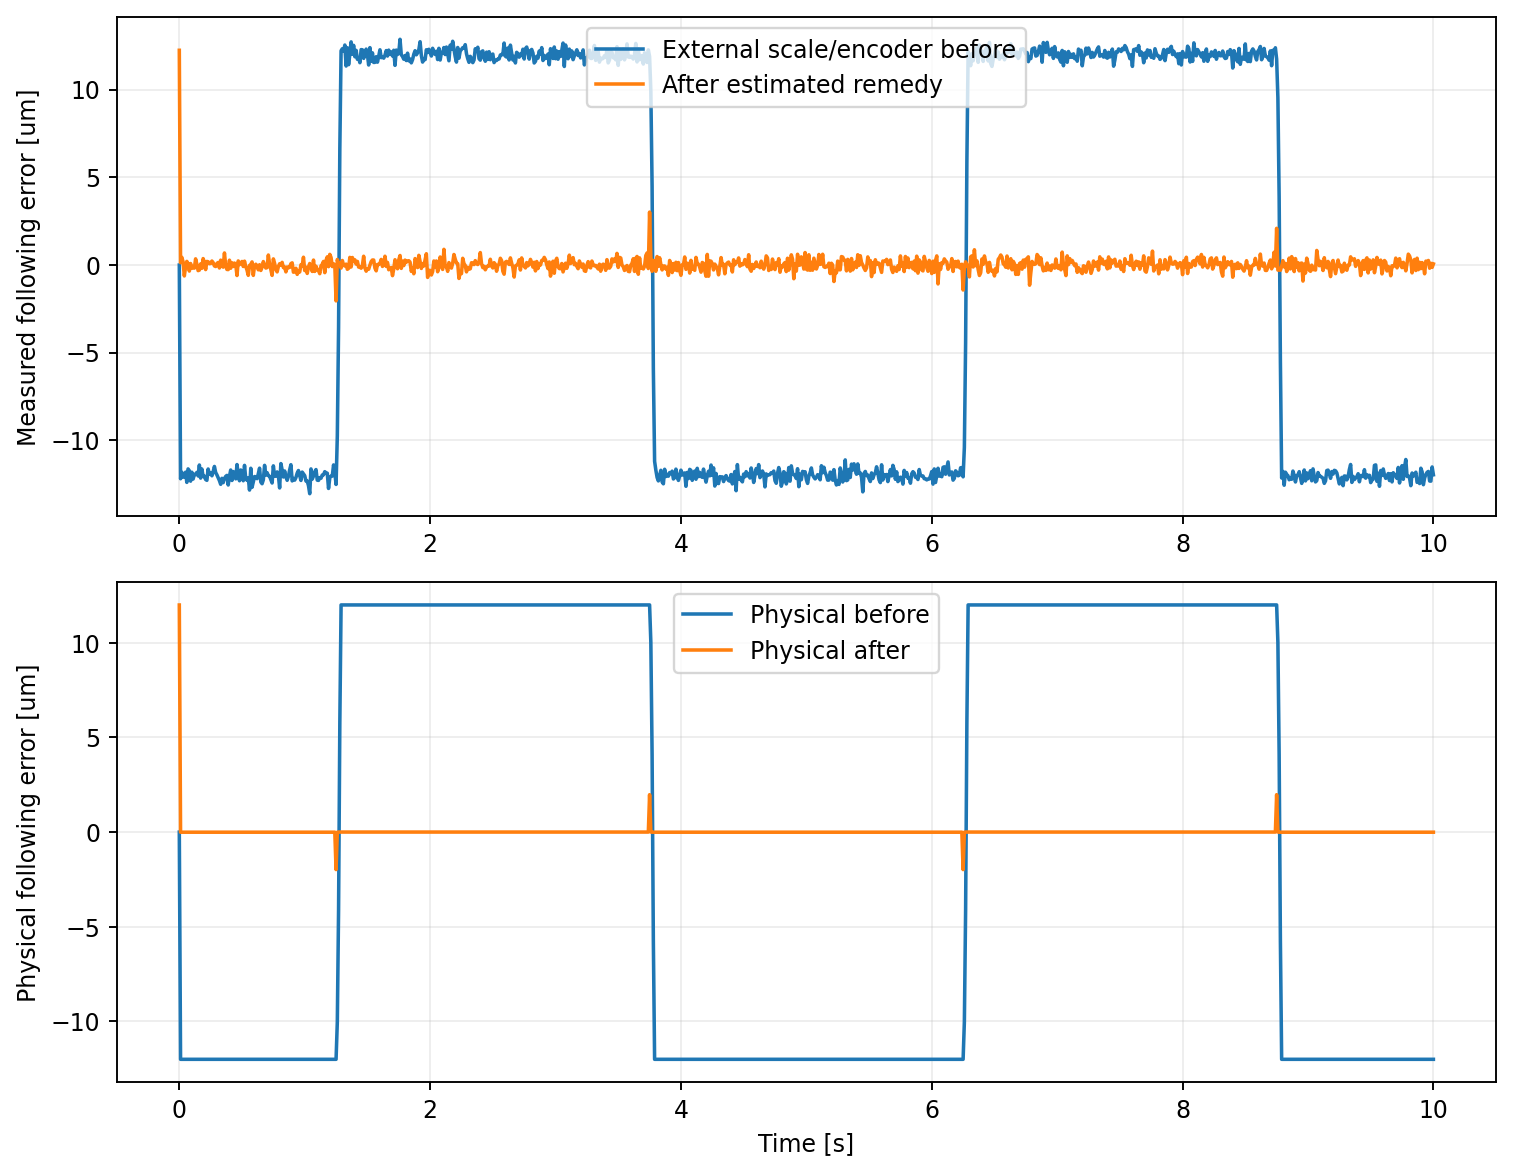
\includegraphics[width=.97\linewidth,height=73mm,keepaspectratio]{figures/backlash.png}\par\small\refstepcounter{figure}\textbf{Figure \thefigure.} External scale error before and after inverse play compensation.\end{center}

\clearpage

\subsection{Lag, offset metrology and missing channels}

For the isolated first-order drive, the identified time constant is 20.001 ms; feedforward reduces physical RMS from 1074.46 to 0.041 micrometres. For Abbe error, $e\simeq h\theta$: independent angle measurement reduces residual RMS from 2.910 to 0.205 micrometres. Median fusion reduces single-channel corruption RMS from 5.730 to 0.375 micrometres; simultaneous common-mode bias would survive that vote.

\par{\small\textit{Implementation}\quad \file{remedies.py}\enspace /\enspace \file{experiments.py}}\par

\begin{center}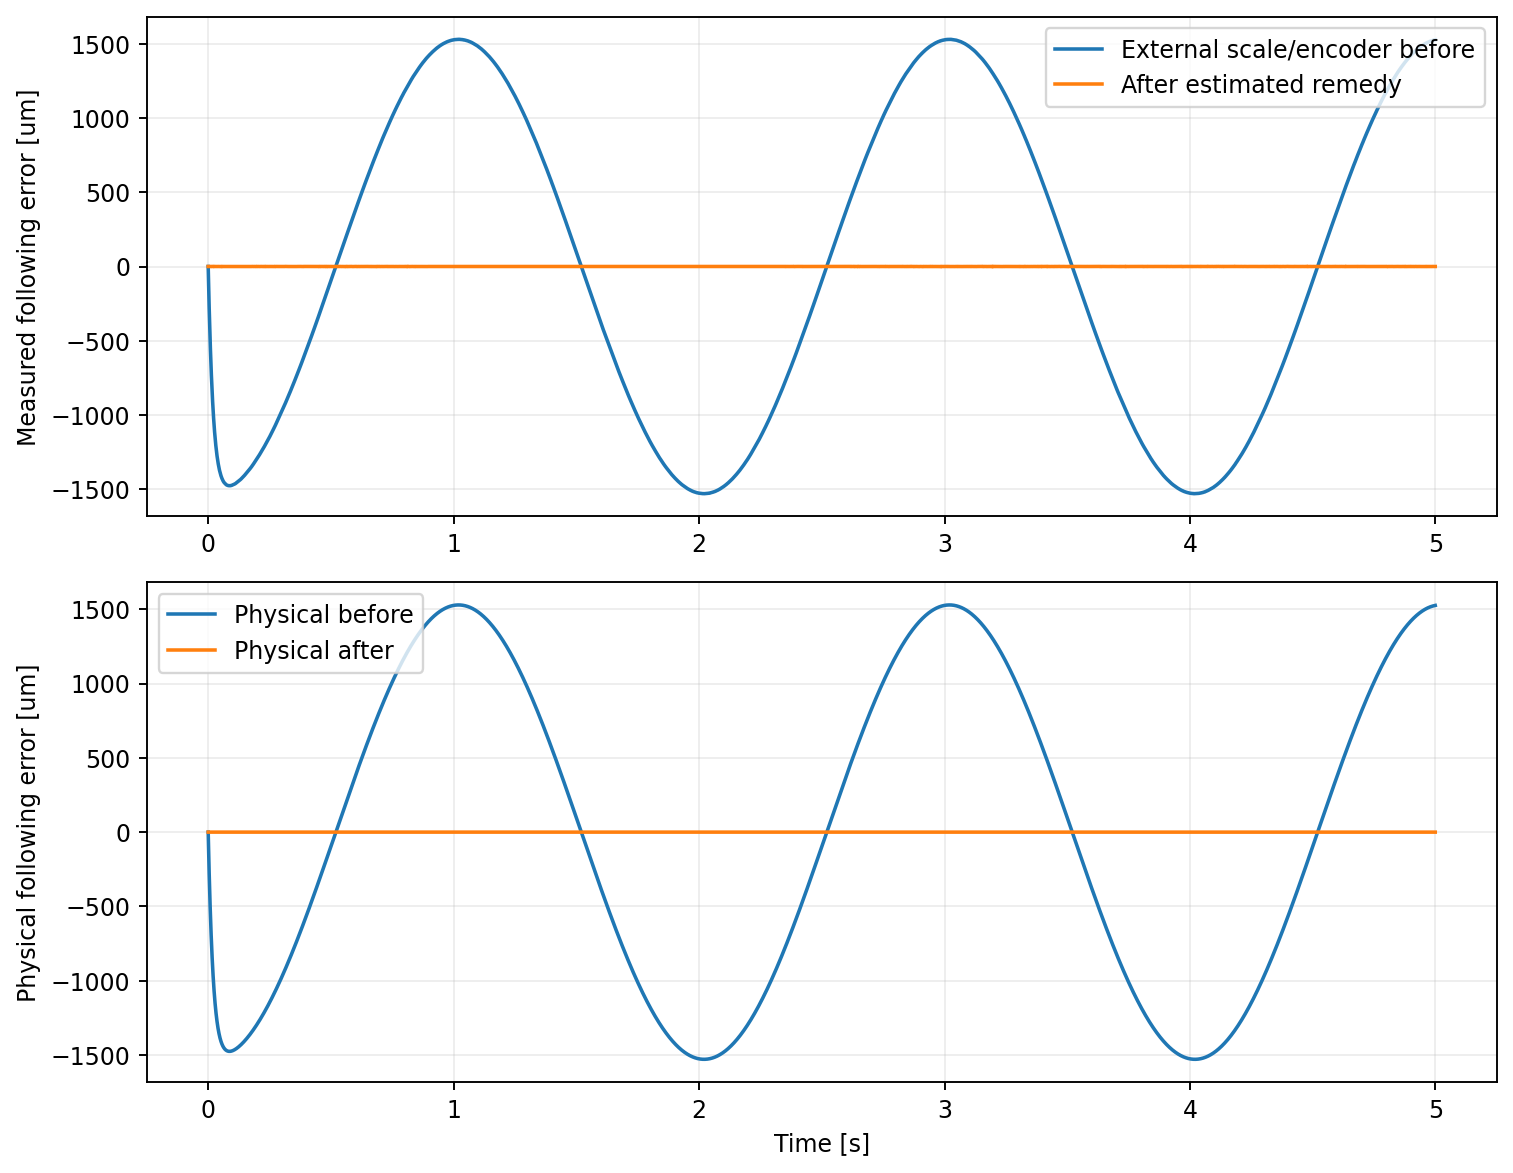
\includegraphics[width=.97\linewidth,height=47mm,keepaspectratio]{figures/servo.png}\par\small\refstepcounter{figure}\textbf{Figure \thefigure.} Sensor noise remains visible after cancellation of the simple plant lag.\end{center}

\begin{center}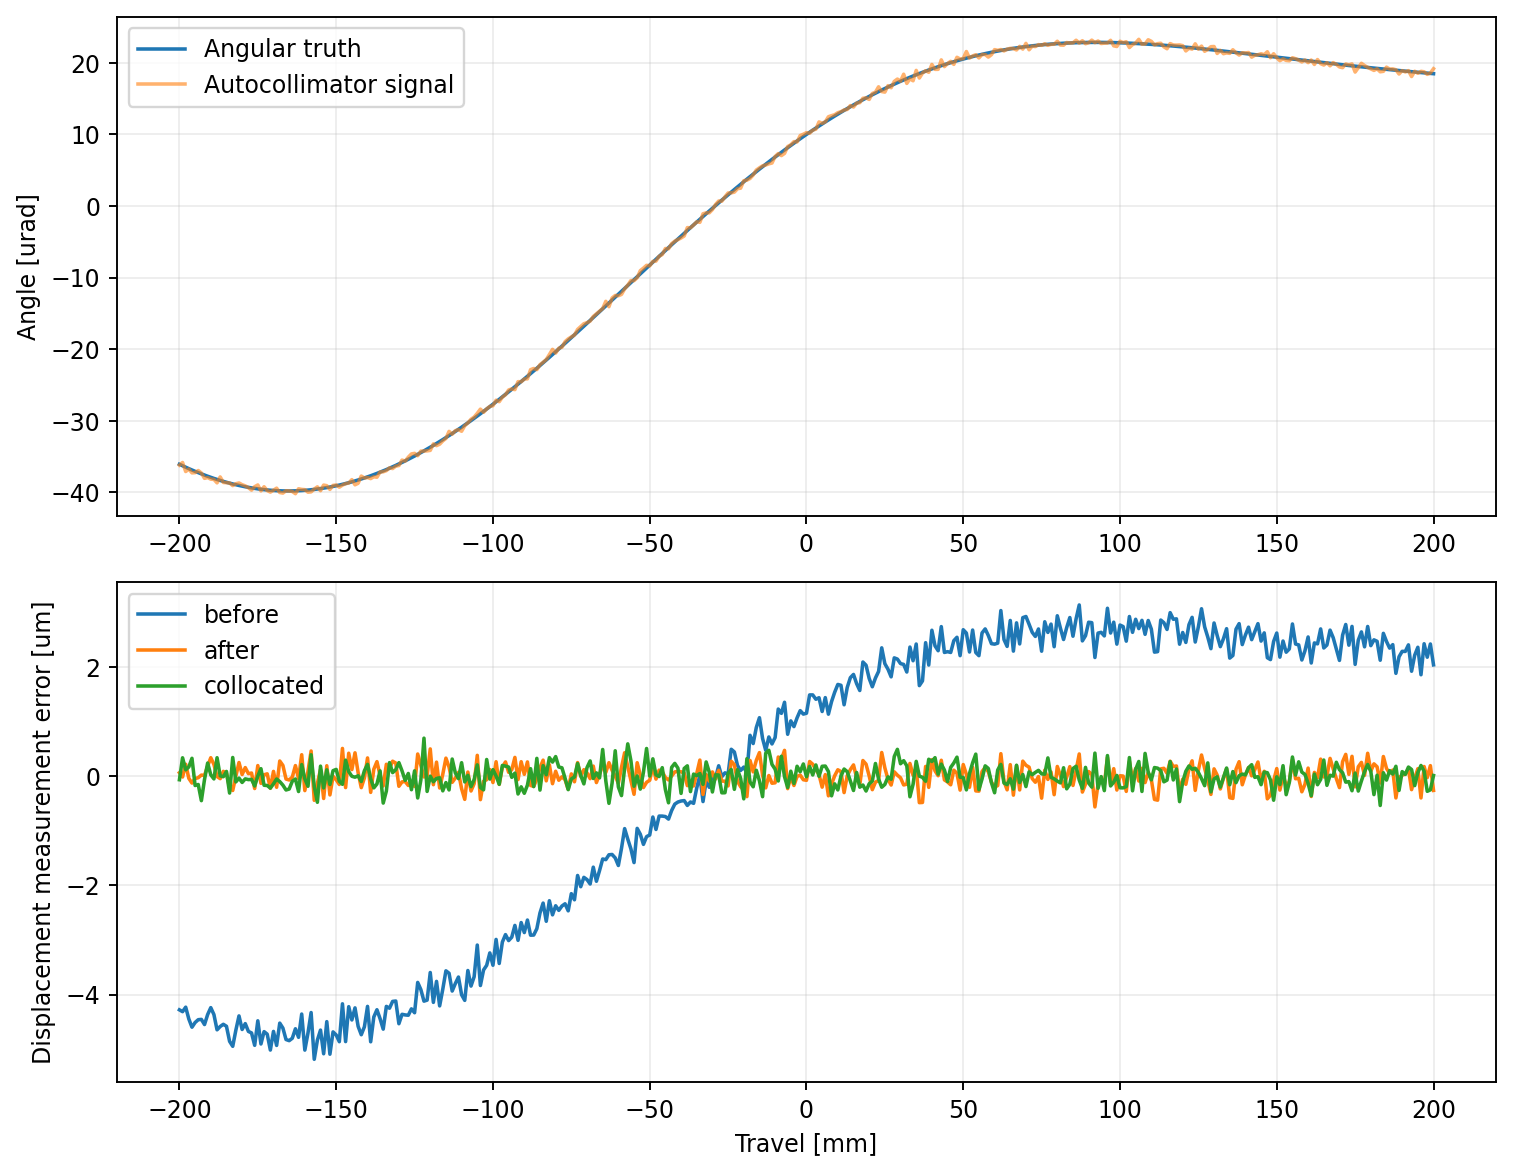
\includegraphics[width=.97\linewidth,height=47mm,keepaspectratio]{figures/abbe.png}\par\small\refstepcounter{figure}\textbf{Figure \thefigure.} Effect of angular measurement and sensor offset on linear readout.\end{center}

\begin{center}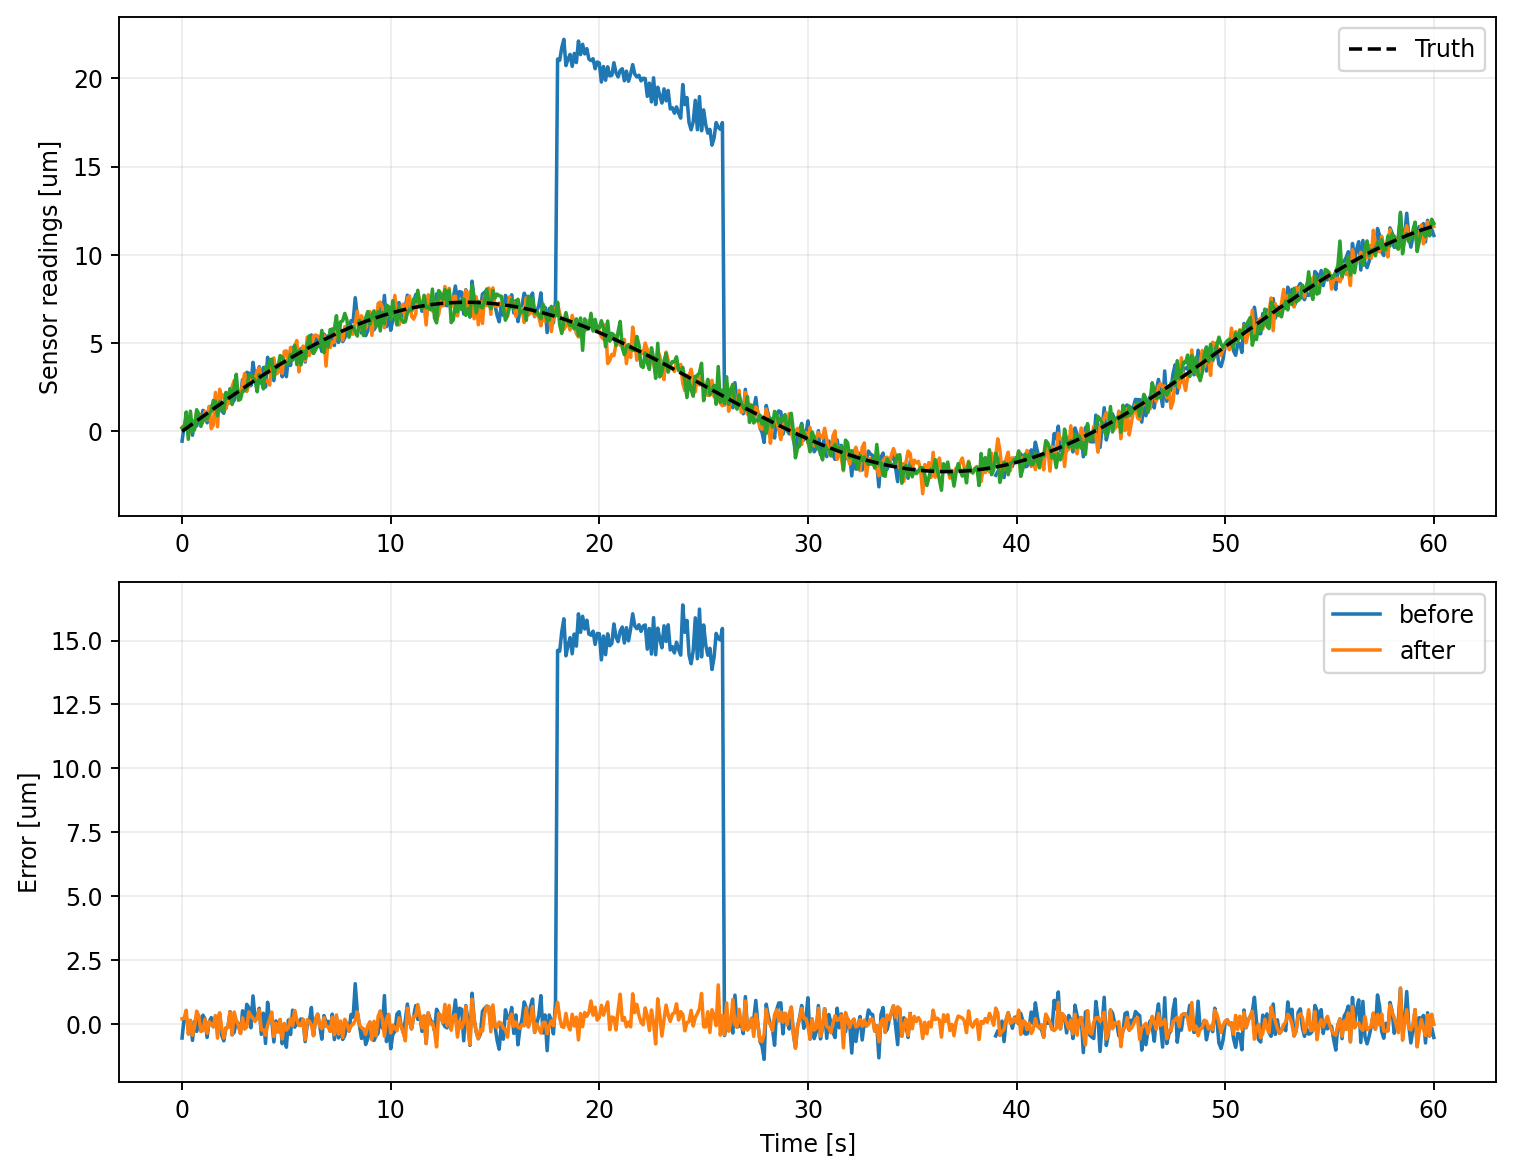
\includegraphics[width=.97\linewidth,height=47mm,keepaspectratio]{figures/sensor_faults.png}\par\small\refstepcounter{figure}\textbf{Figure \thefigure.} Three channels, a corrupted interval and a missing interval.\end{center}

\clearpage

\subsection{Extrapolating the rotating table}

The earlier independent-plant study calibrates cubic and periodic representations on the same 60 poses. The independent frame calculation then evaluates a held-out trajectory. Three-turn TCP RMS is 1878.680 micrometres with an unwrapped cubic and 1.561 with the periodic map on this example. Table 1 earlier in this report averages a different, broader protocol.

\par{\small\textit{Implementation}\quad \file{periodic_model.py}\enspace /\enspace \file{independent_plant.py}\enspace /\enspace \file{research_experiments.py}}\par

\begin{center}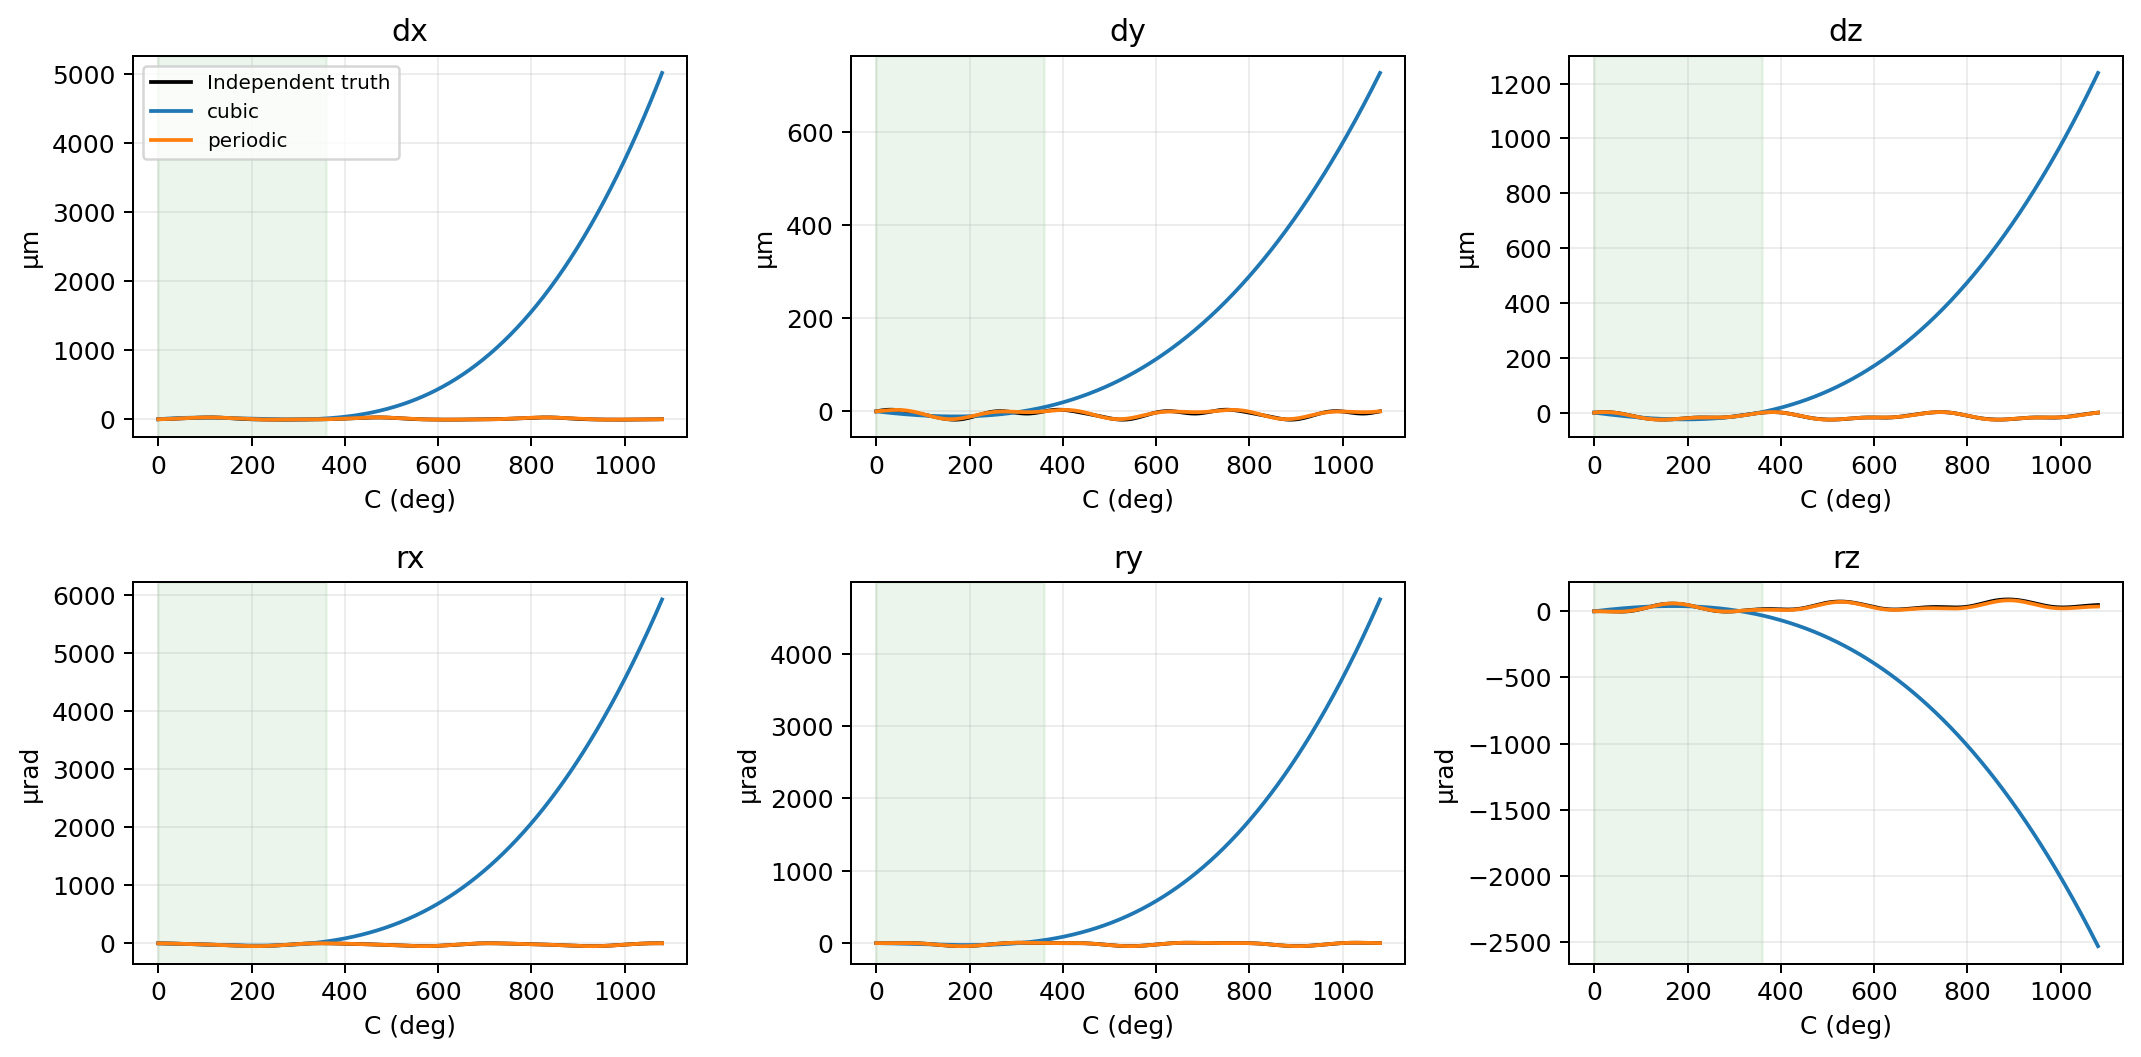
\includegraphics[width=.97\linewidth,height=73mm,keepaspectratio]{figures/research_periodic_maps.png}\par\small\refstepcounter{figure}\textbf{Figure \thefigure.} Fitted rotary channels within and beyond the training revolution.\end{center}

\begin{center}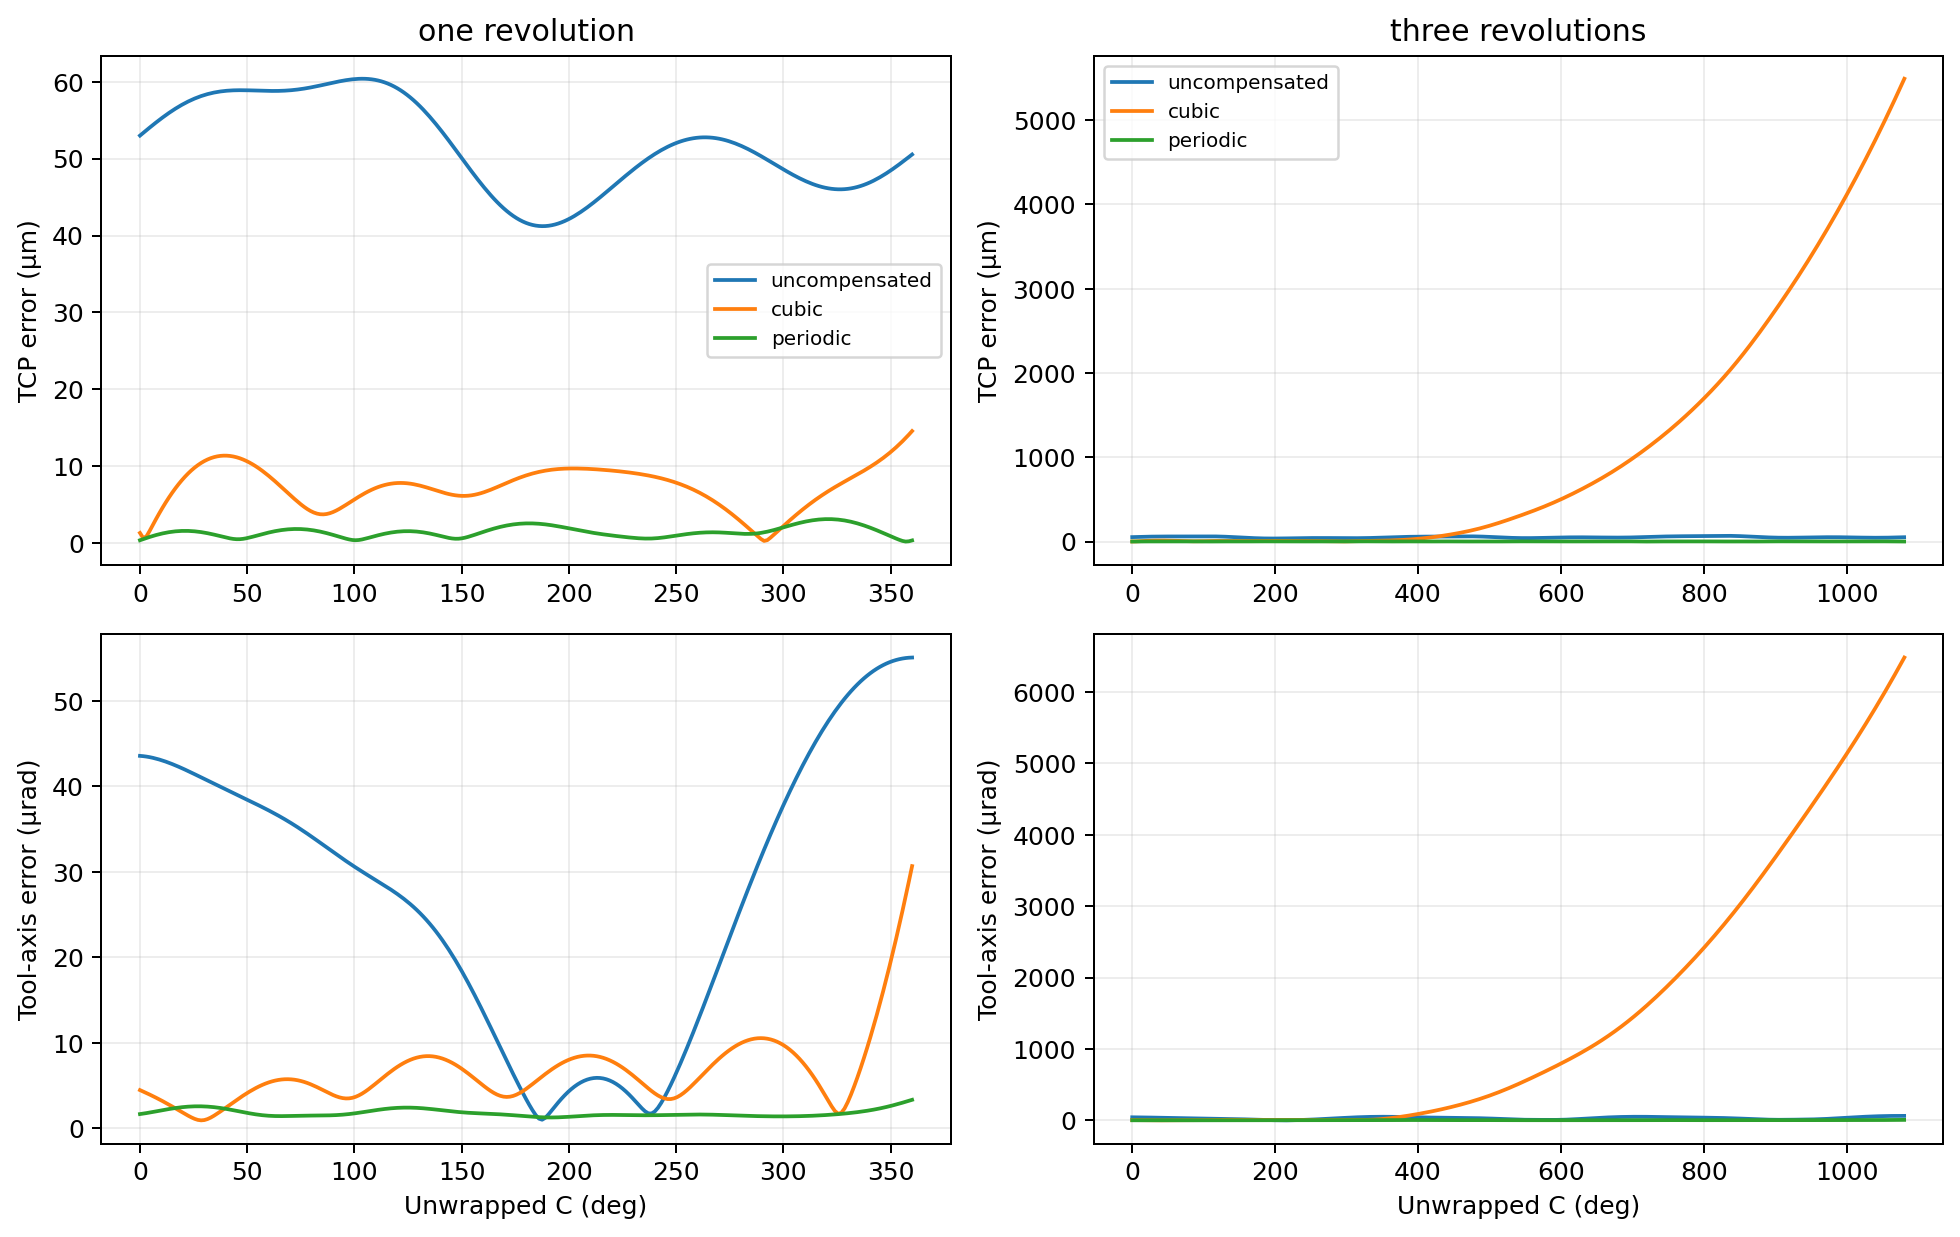
\includegraphics[width=.97\linewidth,height=73mm,keepaspectratio]{figures/research_generalization.png}\par\small\refstepcounter{figure}\textbf{Figure \thefigure.} Static TCP tracking over one and three revolutions.\end{center}

\clearpage

\subsection{Choosing calibration poses}

D-optimal selection adds the pose that most increases the log determinant of the information matrix. Space-filling selection spreads observations over normalized tilt, azimuth, height and radius. The early 24-trial design study holds auxiliary calibration fixed. Its error bars describe repeated measurements on that setup. The right-hand noise prediction explains why adding readings has a diminishing return when geometric mismatch remains.

\par{\small\textit{Implementation}\quad \file{periodic_model.py}\enspace /\enspace \file{research_experiments.py}}\par

\begin{center}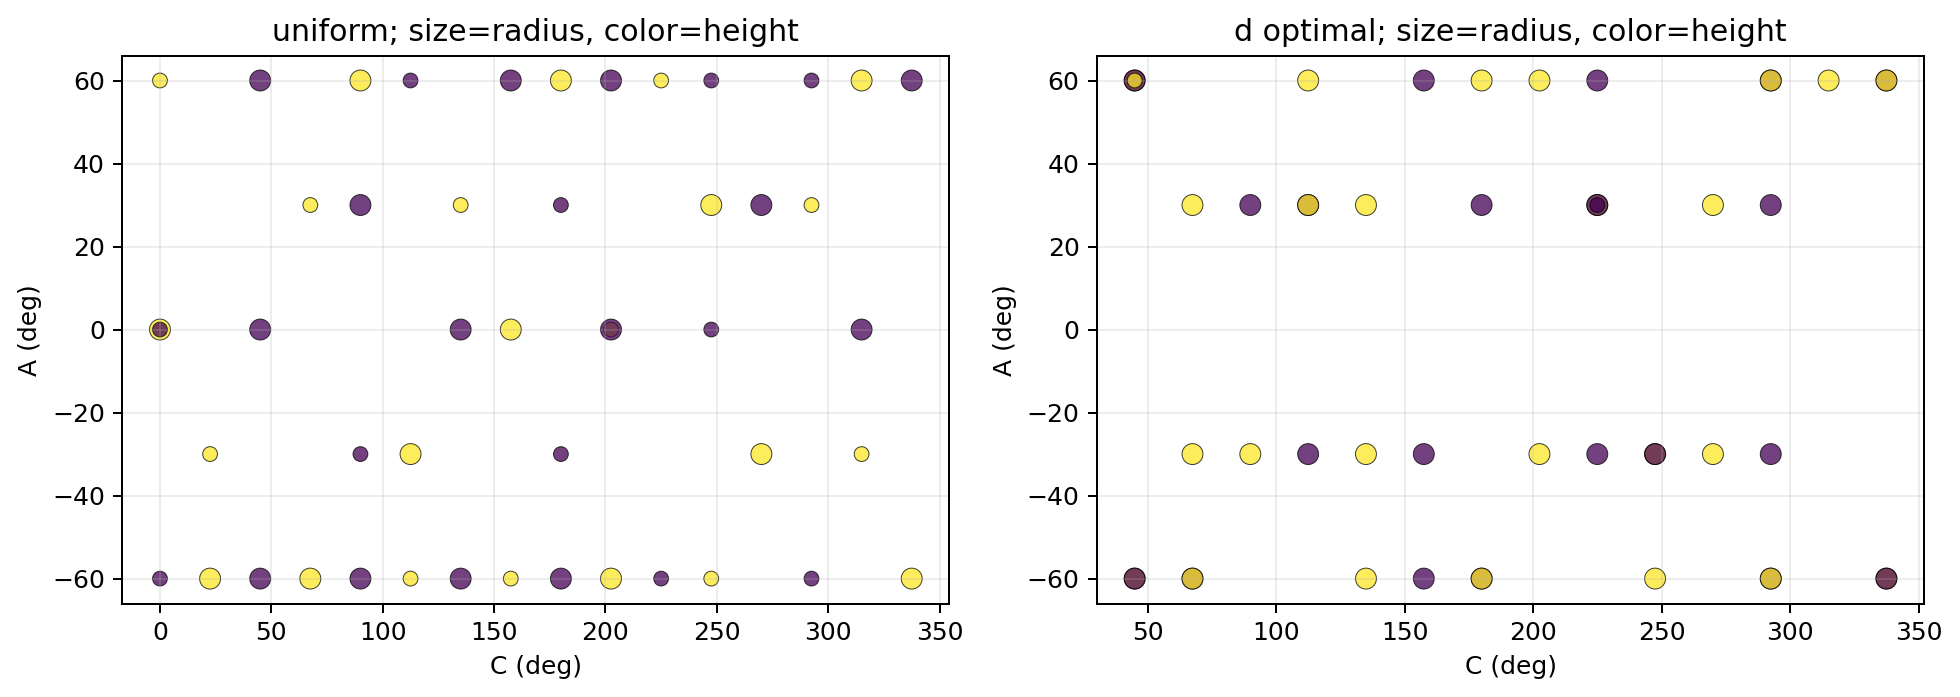
\includegraphics[width=.97\linewidth,height=73mm,keepaspectratio]{figures/research_pose_selection.png}\par\small\refstepcounter{figure}\textbf{Figure \thefigure.} Two 48-pose selections from the same candidate set.\end{center}

\begin{center}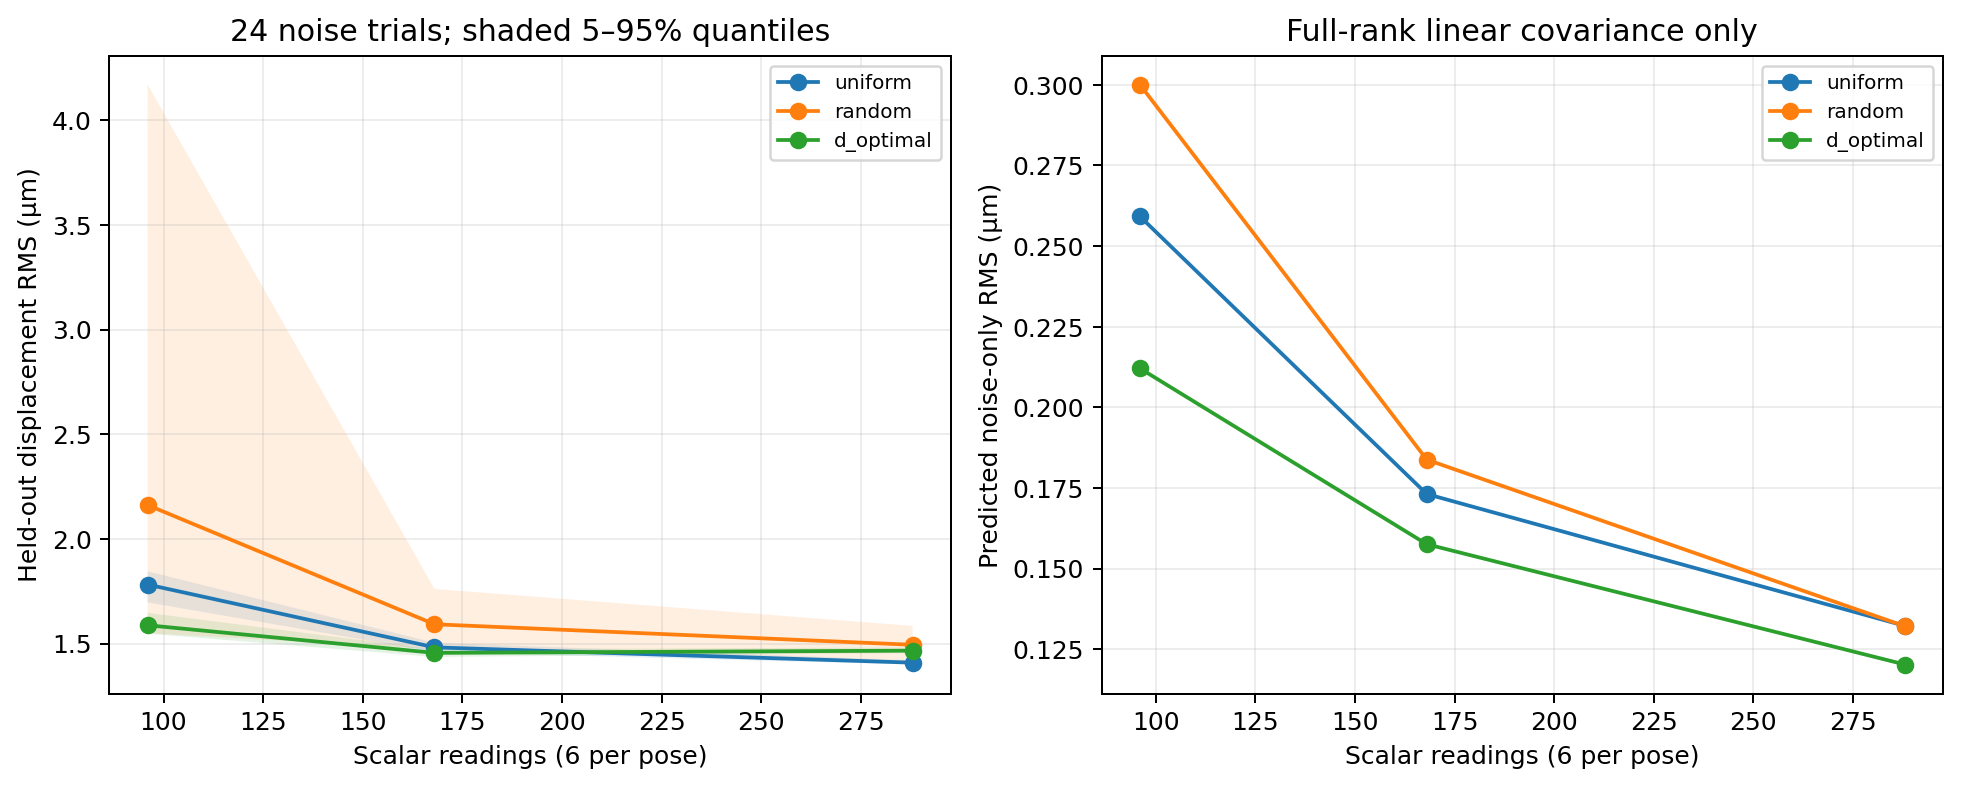
\includegraphics[width=.97\linewidth,height=73mm,keepaspectratio]{figures/research_design.png}\par\small\refstepcounter{figure}\textbf{Figure \thefigure.} Held-out displacement RMS and the conditional noise contribution.\end{center}

\clearpage

\subsection{How to spend a scalar-reading budget}

At fixed zero tilt, the 18 A-axis map columns vanish, leaving rank 25/43. With varied tilt, position-only observations already reach 43/43. Buying three more angle readings per pose then trades independent directions against workspace coverage. At a budget of 288 scalar readings, position-only sampling permits 96 poses and yields 0.107 micrometres noise RMS; six-channel sampling permits 48 poses and yields 0.118 in the task I-optimal comparison.

\par{\small\textit{Implementation}\quad \file{publication_studies.py}\enspace /\enspace \file{research_dashboard.py}}\par

\begin{center}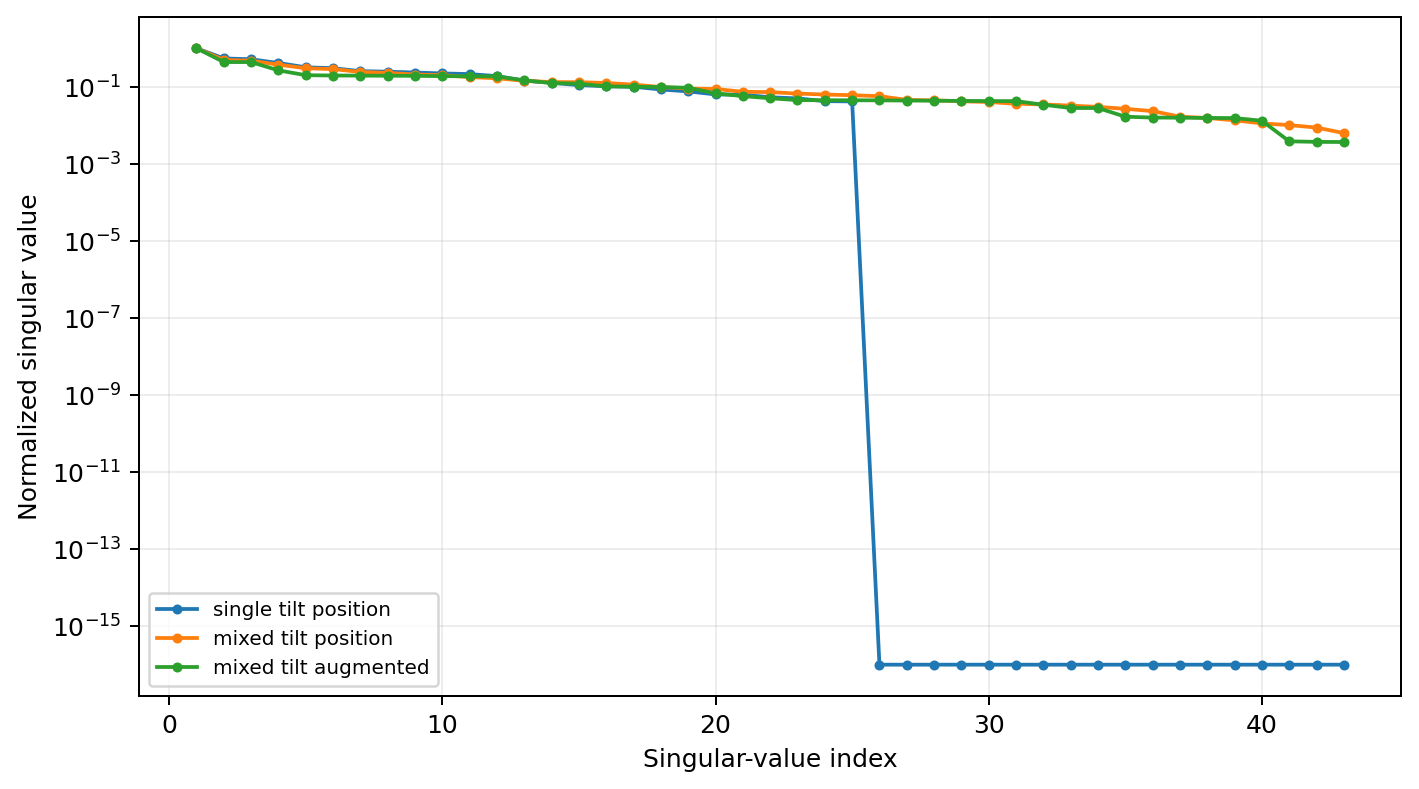
\includegraphics[width=.97\linewidth,height=73mm,keepaspectratio]{figures/research_observability.png}\par\small\refstepcounter{figure}\textbf{Figure \thefigure.} Singular spectra under tilt restriction and different observation channels.\end{center}

\begin{center}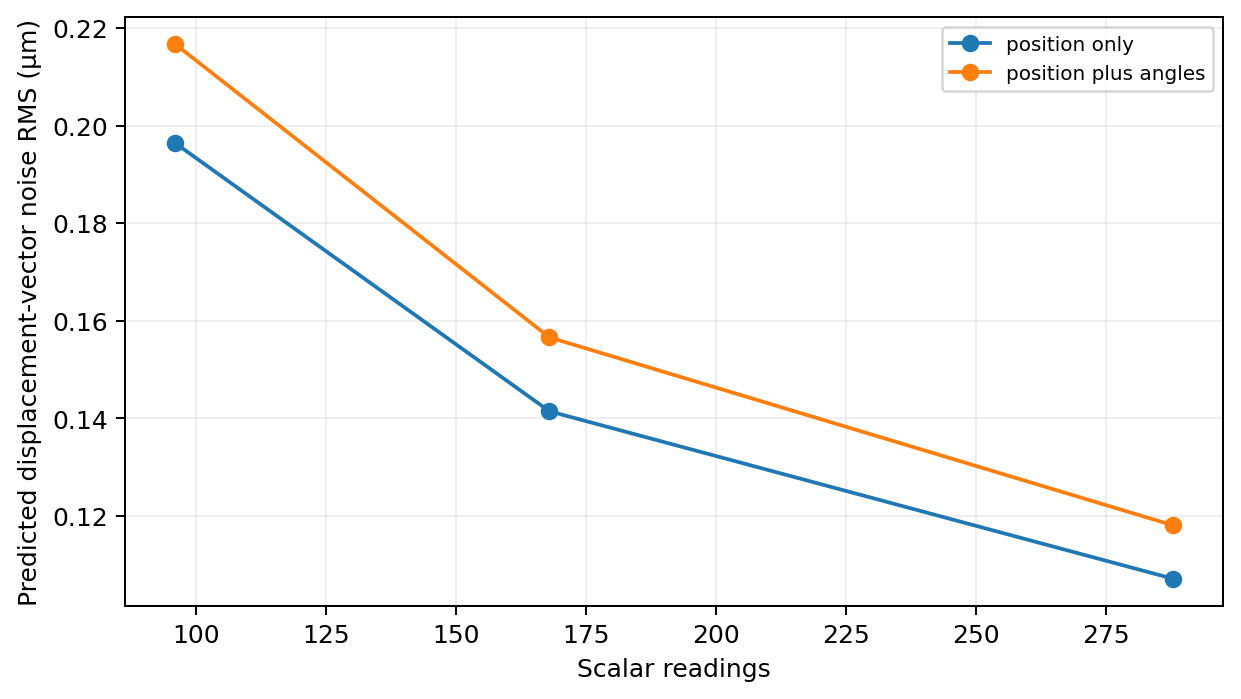
\includegraphics[width=.97\linewidth,height=73mm,keepaspectratio]{figures/publication_sensor_budget.png}\par\small\refstepcounter{figure}\textbf{Figure \thefigure.} Equal-reading comparison across three budgets.\end{center}

\clearpage

\subsection{Separating design noise from omitted geometry}

In the expanded study, seed, configuration, design, omitted-error amplitude and noise draw are varied. With 48 poses and unit omission amplitude, D-optimal selection gives 1.244 micrometres total RMS, including 1.228 micrometres noiseless bias. At triple amplitude the corresponding values are 3.689 and 3.683. The predicted rotary-noise component stays at 0.125 because it depends on the fitted sensitivity and sensor law.

\par{\small\textit{Implementation}\quad \file{publication_studies.py}}\par

\begin{center}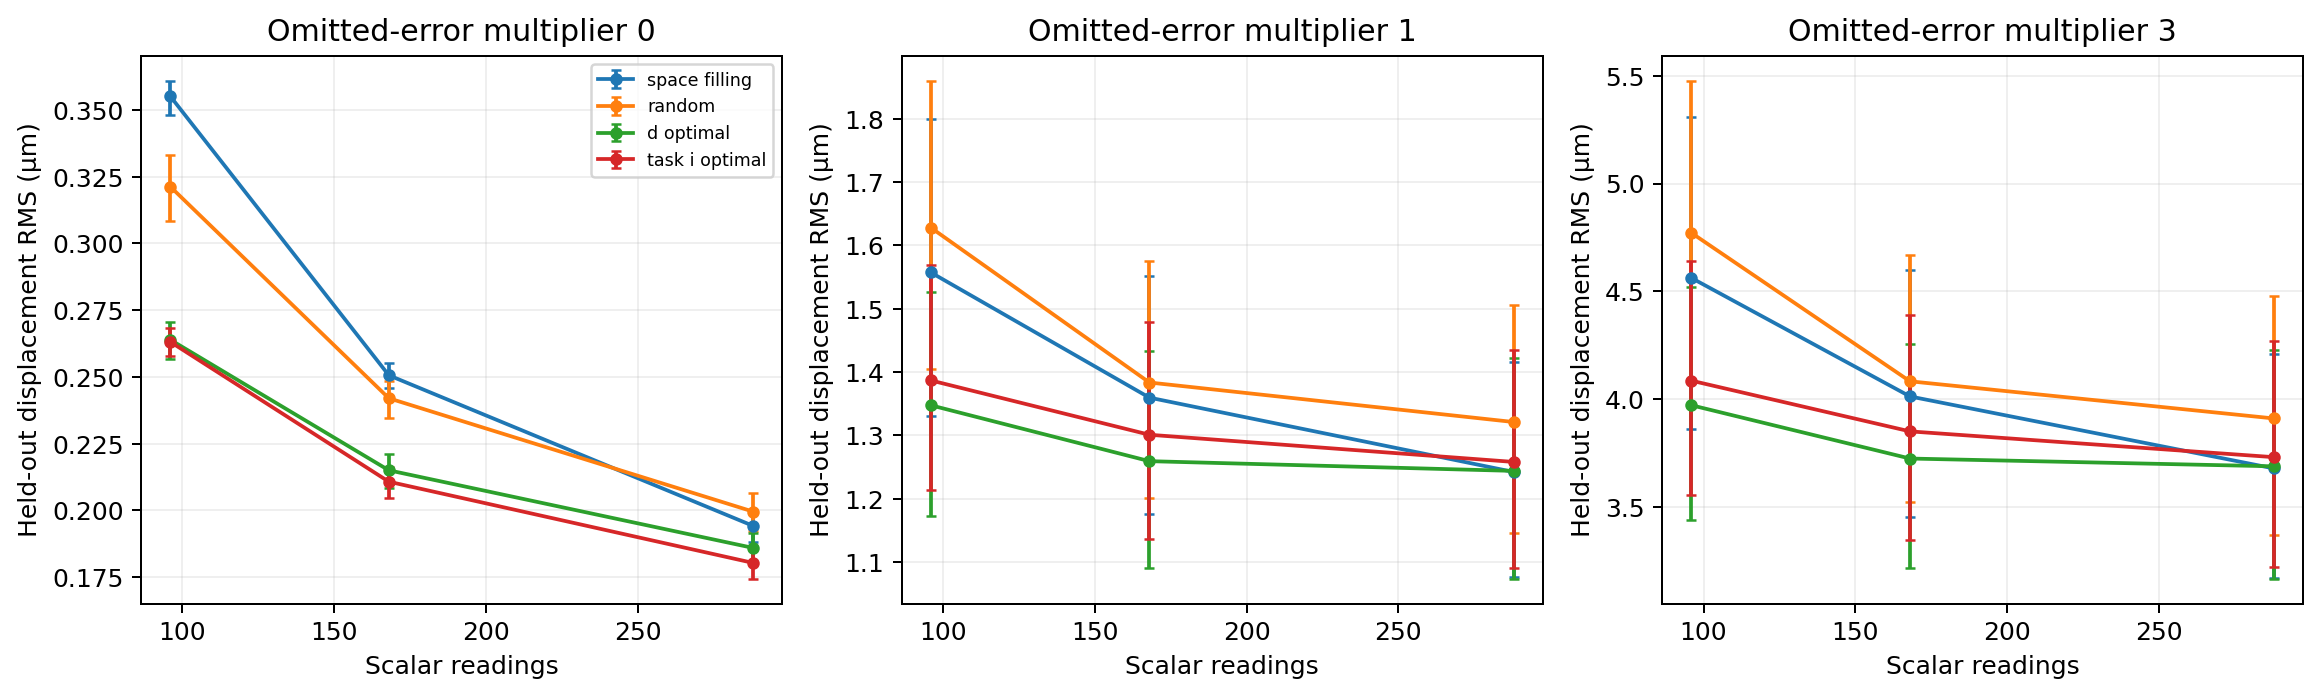
\includegraphics[width=.97\linewidth,height=73mm,keepaspectratio]{figures/publication_design_panel.png}\par\small\refstepcounter{figure}\textbf{Figure \thefigure.} Paired, equal-budget assessment across designs and truth configurations.\end{center}

\begin{center}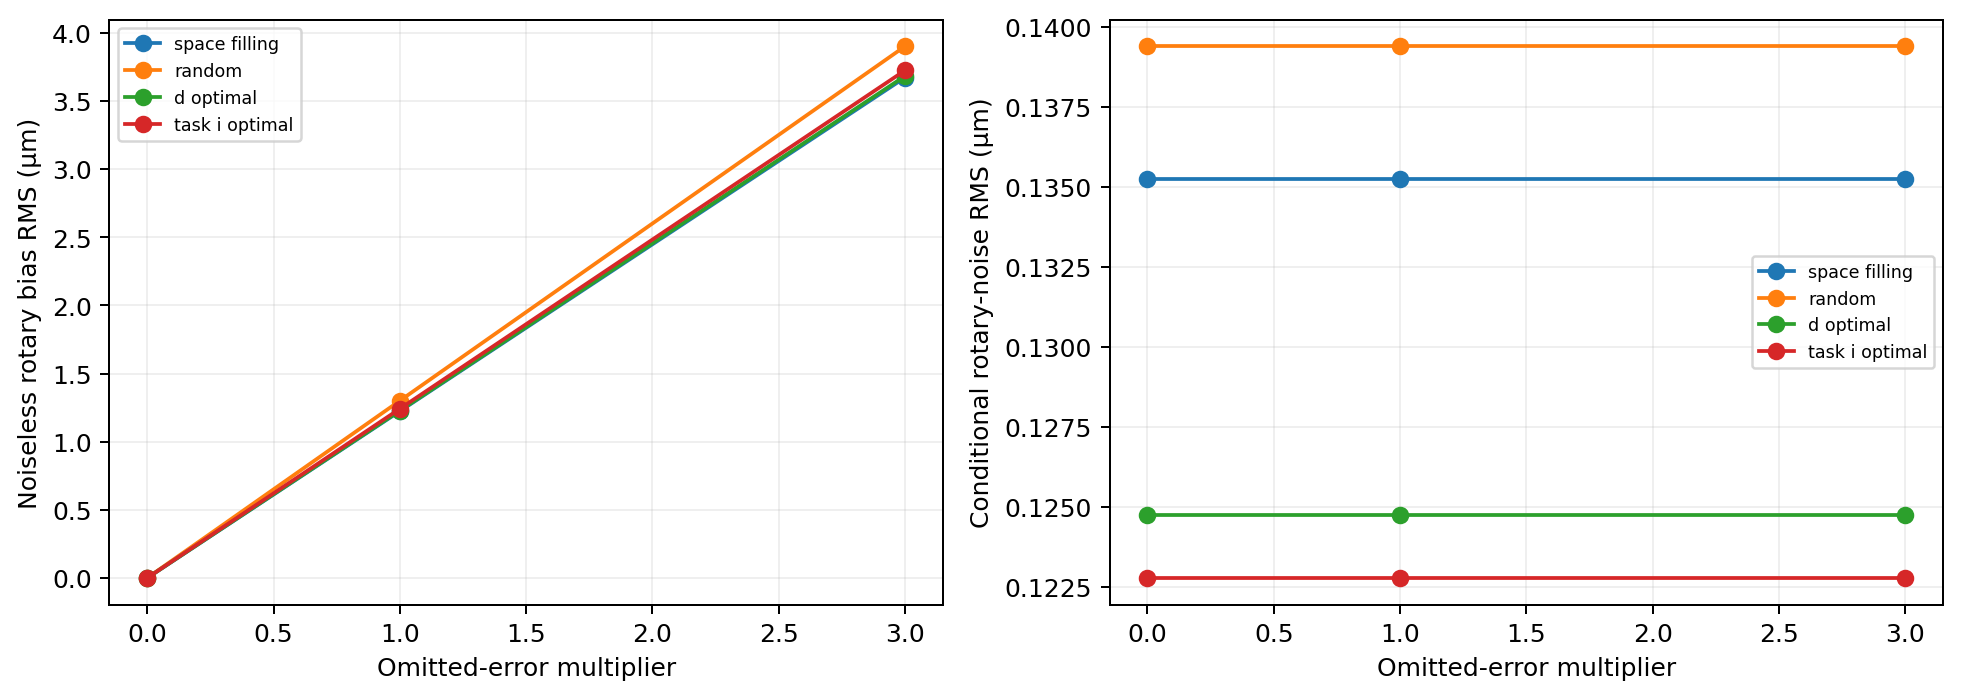
\includegraphics[width=.97\linewidth,height=73mm,keepaspectratio]{figures/publication_bias_variance.png}\par\small\refstepcounter{figure}\textbf{Figure \thefigure.} Noise-only and noiseless terms as omitted-error amplitude increases.\end{center}

\clearpage

\subsection{A fairer rotary representation comparison}

Wrapping the cubic at each revolution tests how much of the multi-turn failure is simple extrapolation. A second control matches the number of coefficients: five- and nine-knot periodic cubic splines match the two- and four-harmonic maps at 43 and 67 parameters. At 67 coefficients on localized truth, the three-turn RMS is 0.533 micrometres for Fourier and 0.597 for the spline. The model families encode different smooth shapes even at equal capacity.

\par{\small\textit{Implementation}\quad \file{publication_studies.py}\enspace /\enspace \file{journal_studies.py}}\par

\begin{center}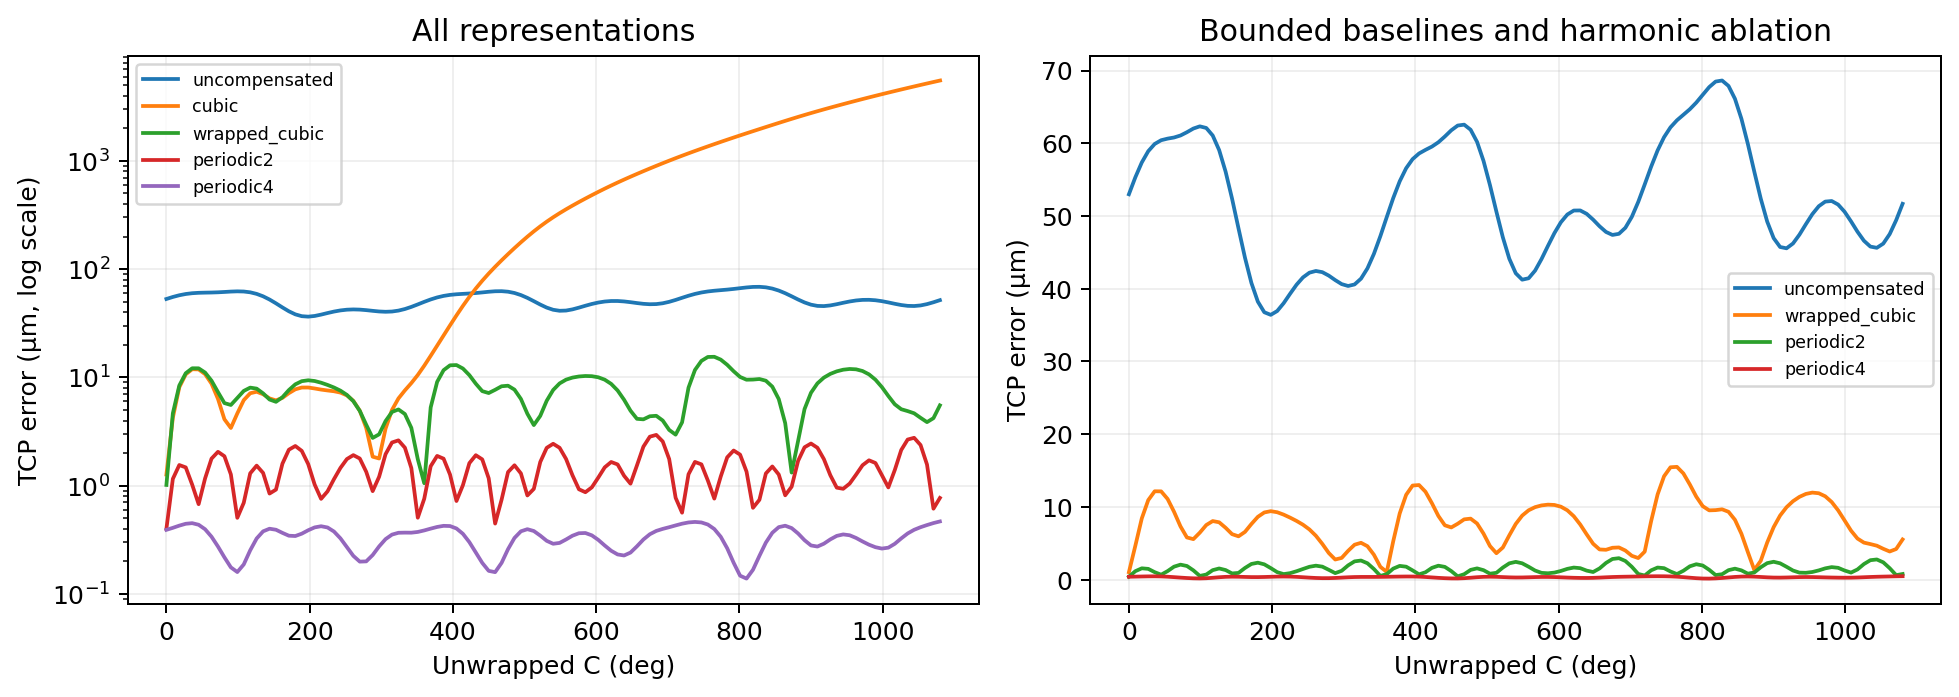
\includegraphics[width=.97\linewidth,height=73mm,keepaspectratio]{figures/publication_wrapped_baseline.png}\par\small\refstepcounter{figure}\textbf{Figure \thefigure.} Wrapped and unwrapped baselines on the same three-turn case.\end{center}

\begin{center}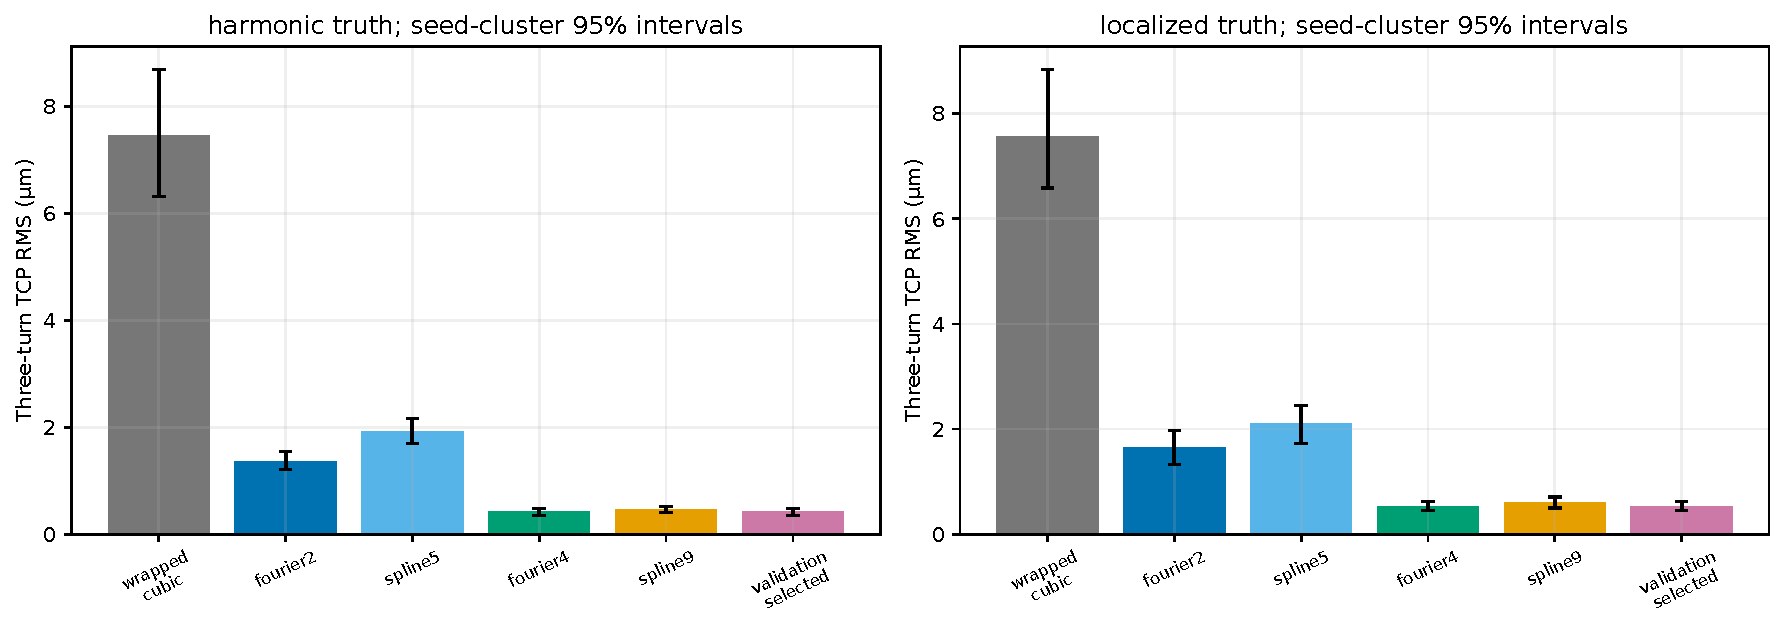
\includegraphics[width=.97\linewidth,height=73mm,keepaspectratio]{figures/journal_equal_capacity.pdf}\par\small\refstepcounter{figure}\textbf{Figure \thefigure.} Comparison under harmonic and localized truth, with seed-cluster intervals.\end{center}

\clearpage

\subsection{Selecting a map using sensor data}

Selection uses 32 disjoint six-channel validation poses. Each candidate is scored on its normalized rotary sensor residuals; the held-out TCP path is reserved for assessment. Across 36 seed/configuration pairs per family, the resulting selected models give three-turn mean RMS of 0.417 micrometres on harmonic truth and 0.533 on localized truth. A validation score can support a model choice without access to exact tool positions.

\par{\small\textit{Implementation}\quad \file{journal_models.py}\enspace /\enspace \file{journal_studies.py}}\par

\begin{center}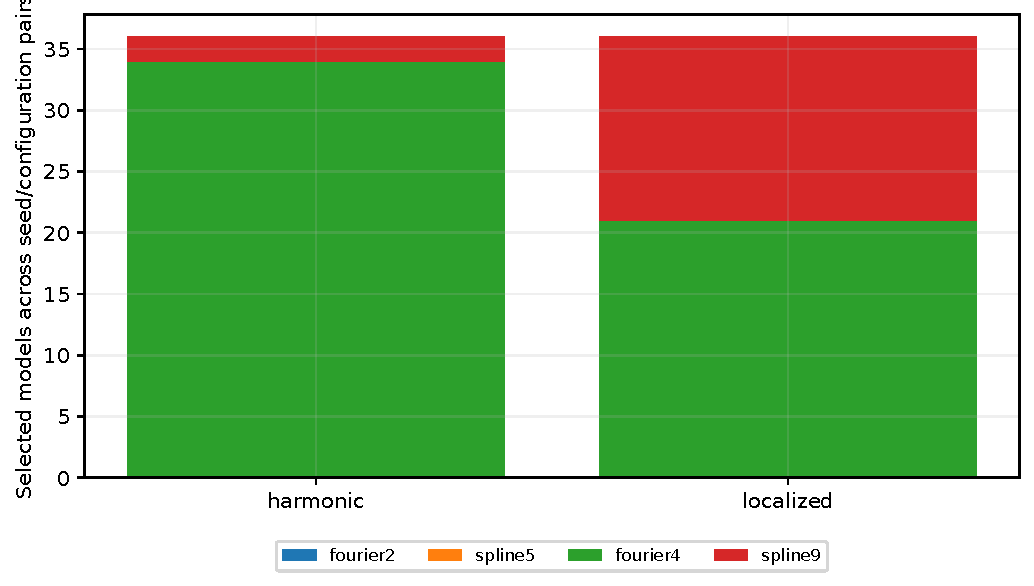
\includegraphics[width=.97\linewidth,height=73mm,keepaspectratio]{figures/journal_model_selection.pdf}\par\small\refstepcounter{figure}\textbf{Figure \thefigure.} Frequency with which each candidate wins on validation readings.\end{center}

\begin{center}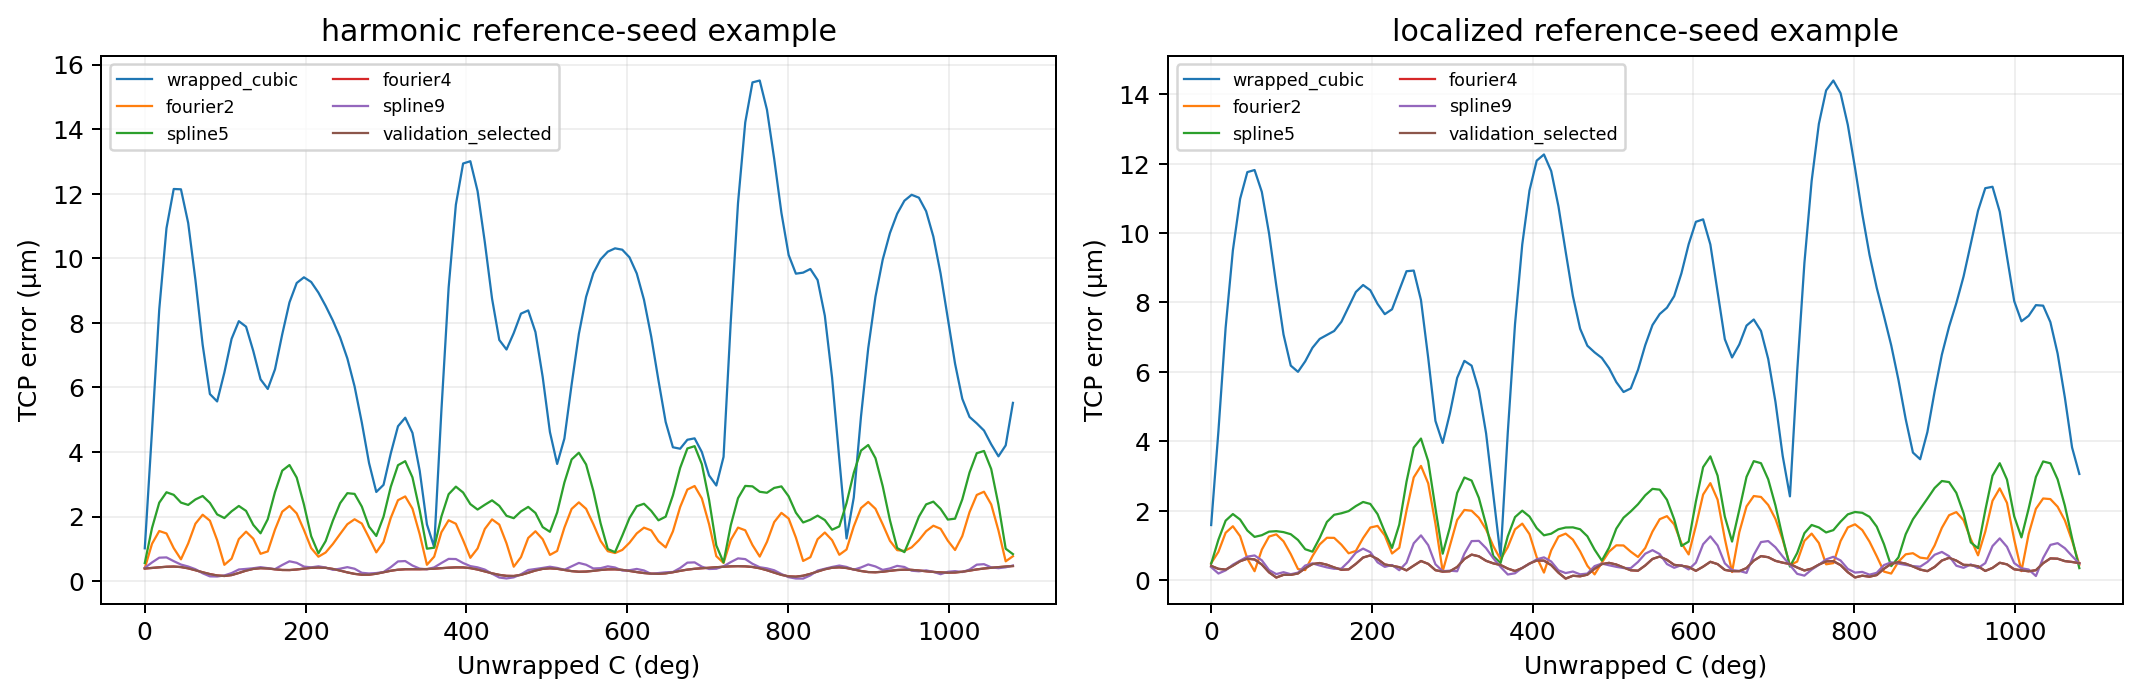
\includegraphics[width=.97\linewidth,height=73mm,keepaspectratio]{figures/journal_family_sensor_traces.png}\par\small\refstepcounter{figure}\textbf{Figure \thefigure.} Position traces on the assessment path for one reference seed.\end{center}

\clearpage

\section{Dynamic execution and independent sensing}

\subsection{Following a moving path}

The early study uses a sequential two-pole lag approximation. On its 30 s trajectory, uncompensated TCP RMS is 330.81 micrometres. Adding geometry, thermal compensation and inverse play gives 287.99; adding feedforward brings it to 44.38. In the slower 60 s case the full-remedy RMS is 29.18. These values belong to the earlier integrator. The following physical-time study uses an exact zero-order-hold (ZOH) update.

\par{\small\textit{Implementation}\quad \file{dynamic_sim.py}\enspace /\enspace \file{research_experiments.py}}\par

\begin{center}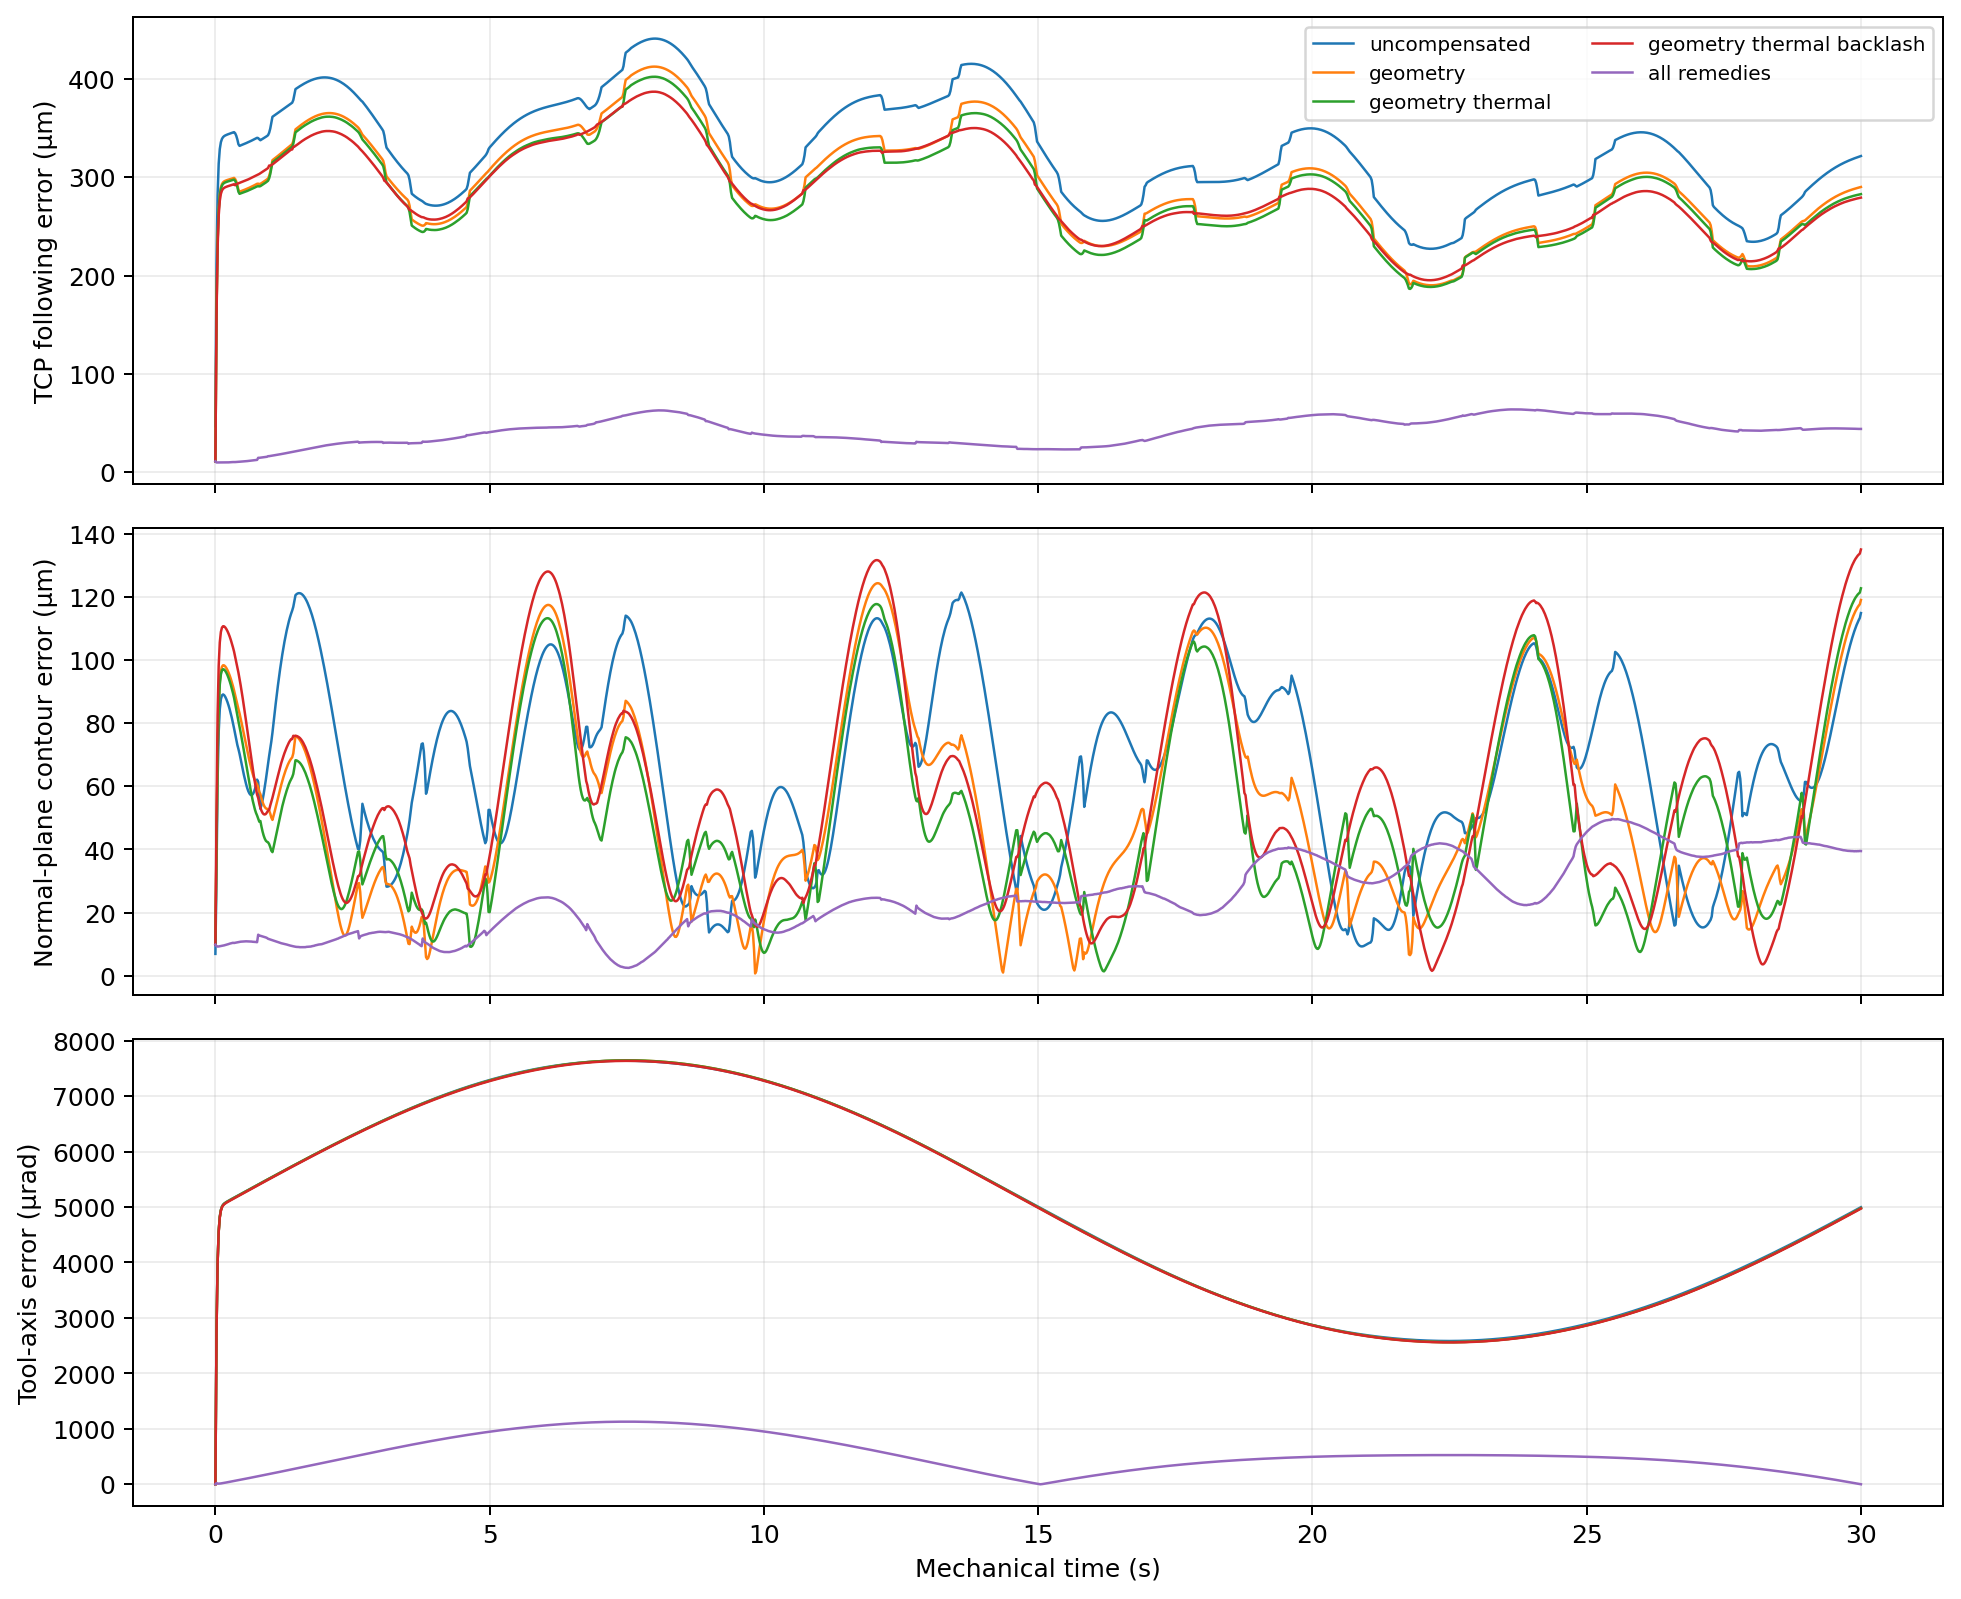
\includegraphics[width=.97\linewidth,height=73mm,keepaspectratio]{figures/research_integrated.png}\par\small\refstepcounter{figure}\textbf{Figure \thefigure.} Cumulative remedies and three trajectory error measures.\end{center}

\begin{center}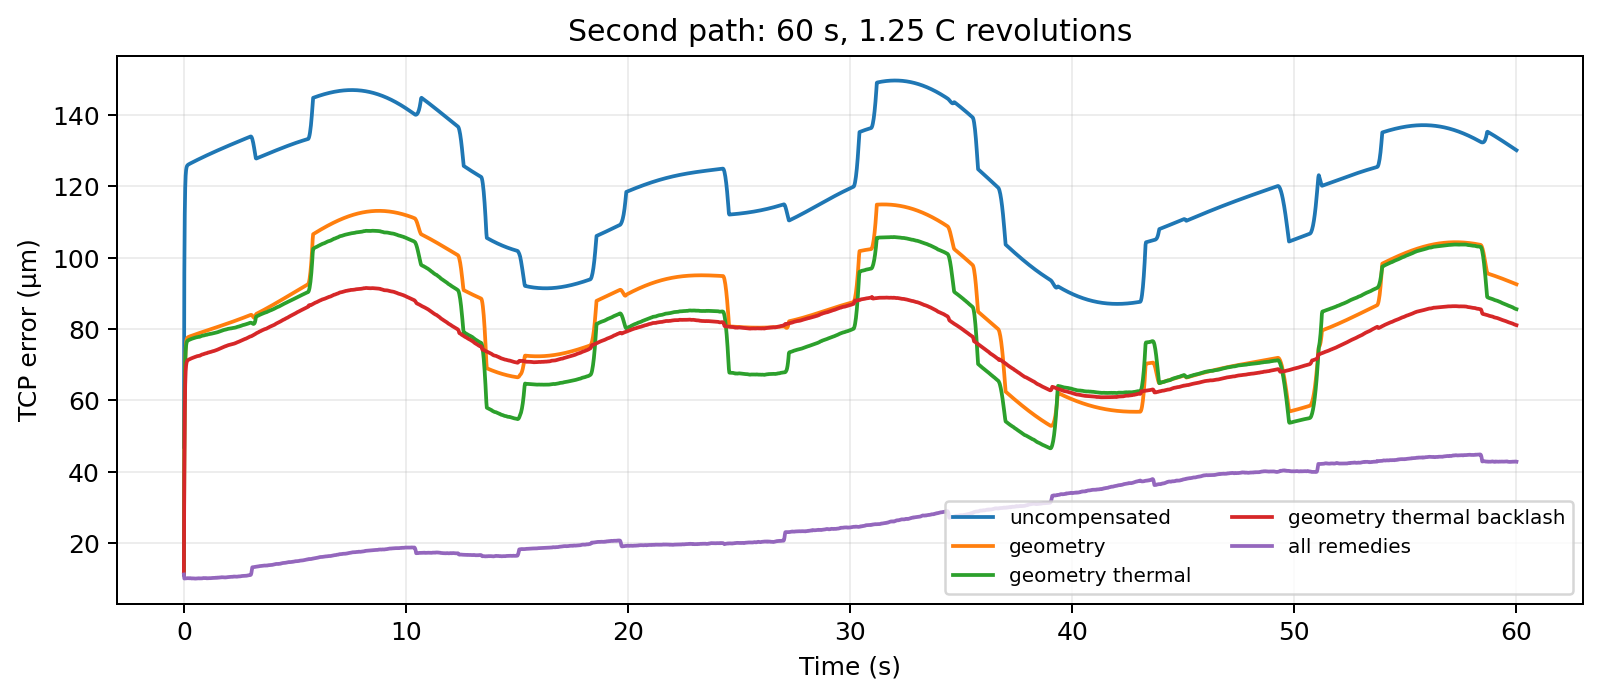
\includegraphics[width=.97\linewidth,height=73mm,keepaspectratio]{figures/research_second_path.png}\par\small\refstepcounter{figure}\textbf{Figure \thefigure.} Held-out slower-path result with the earlier drive model.\end{center}

\clearpage

\subsection{Which measurement observes which error?}

The drive command, motor encoder and output scale describe different points in the mechanical chain. The command-to-motor residual mainly exposes drive tracking, while output-minus-motor reveals play. Temperature channels are used to estimate drift. A separate XYZ probe evaluates the final motion; using it to tune the same trace would invalidate its role as an independent assessment.

\par{\small\textit{Implementation}\quad \file{dynamic_sim.py}\enspace /\enspace \file{research_experiments.py}}\par

\begin{center}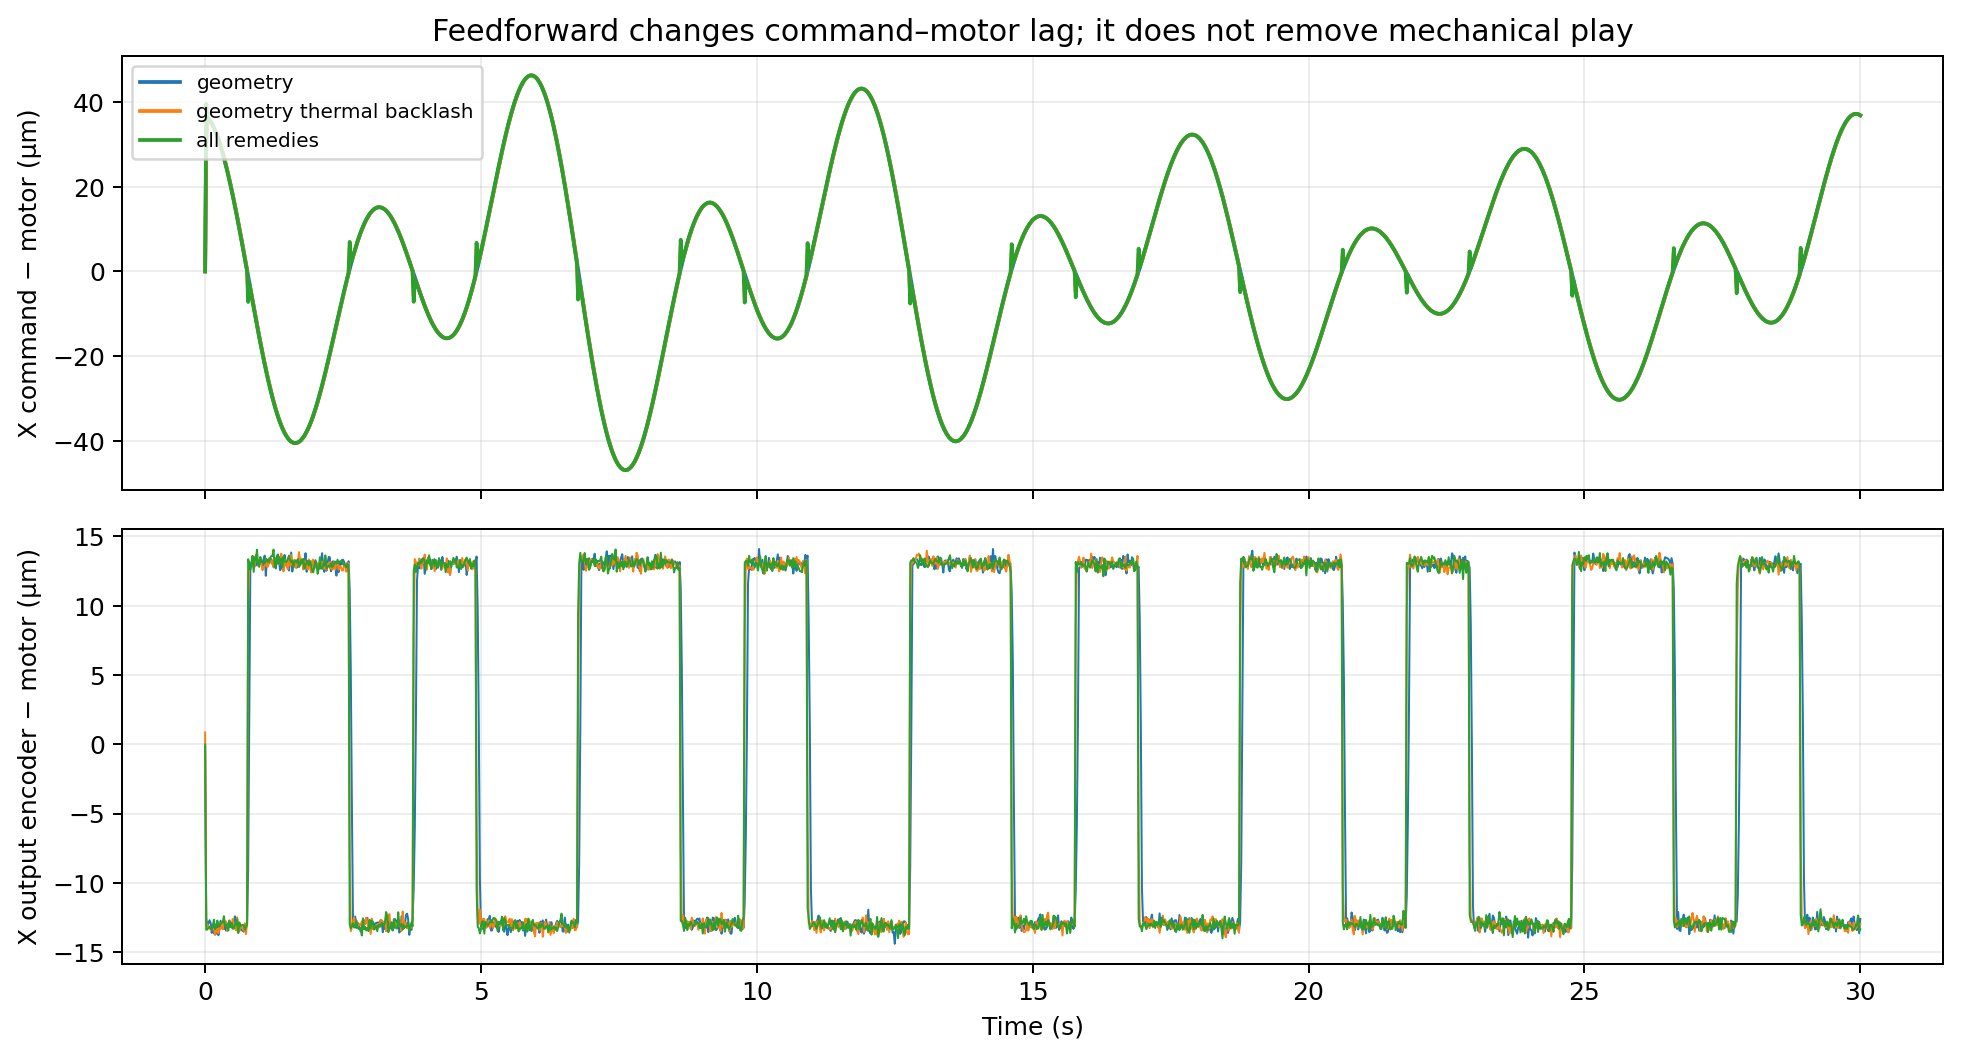
\includegraphics[width=.97\linewidth,height=73mm,keepaspectratio]{figures/research_encoder_sensors.png}\par\small\refstepcounter{figure}\textbf{Figure \thefigure.} Differences between motor and output measurements near reversals.\end{center}

\begin{center}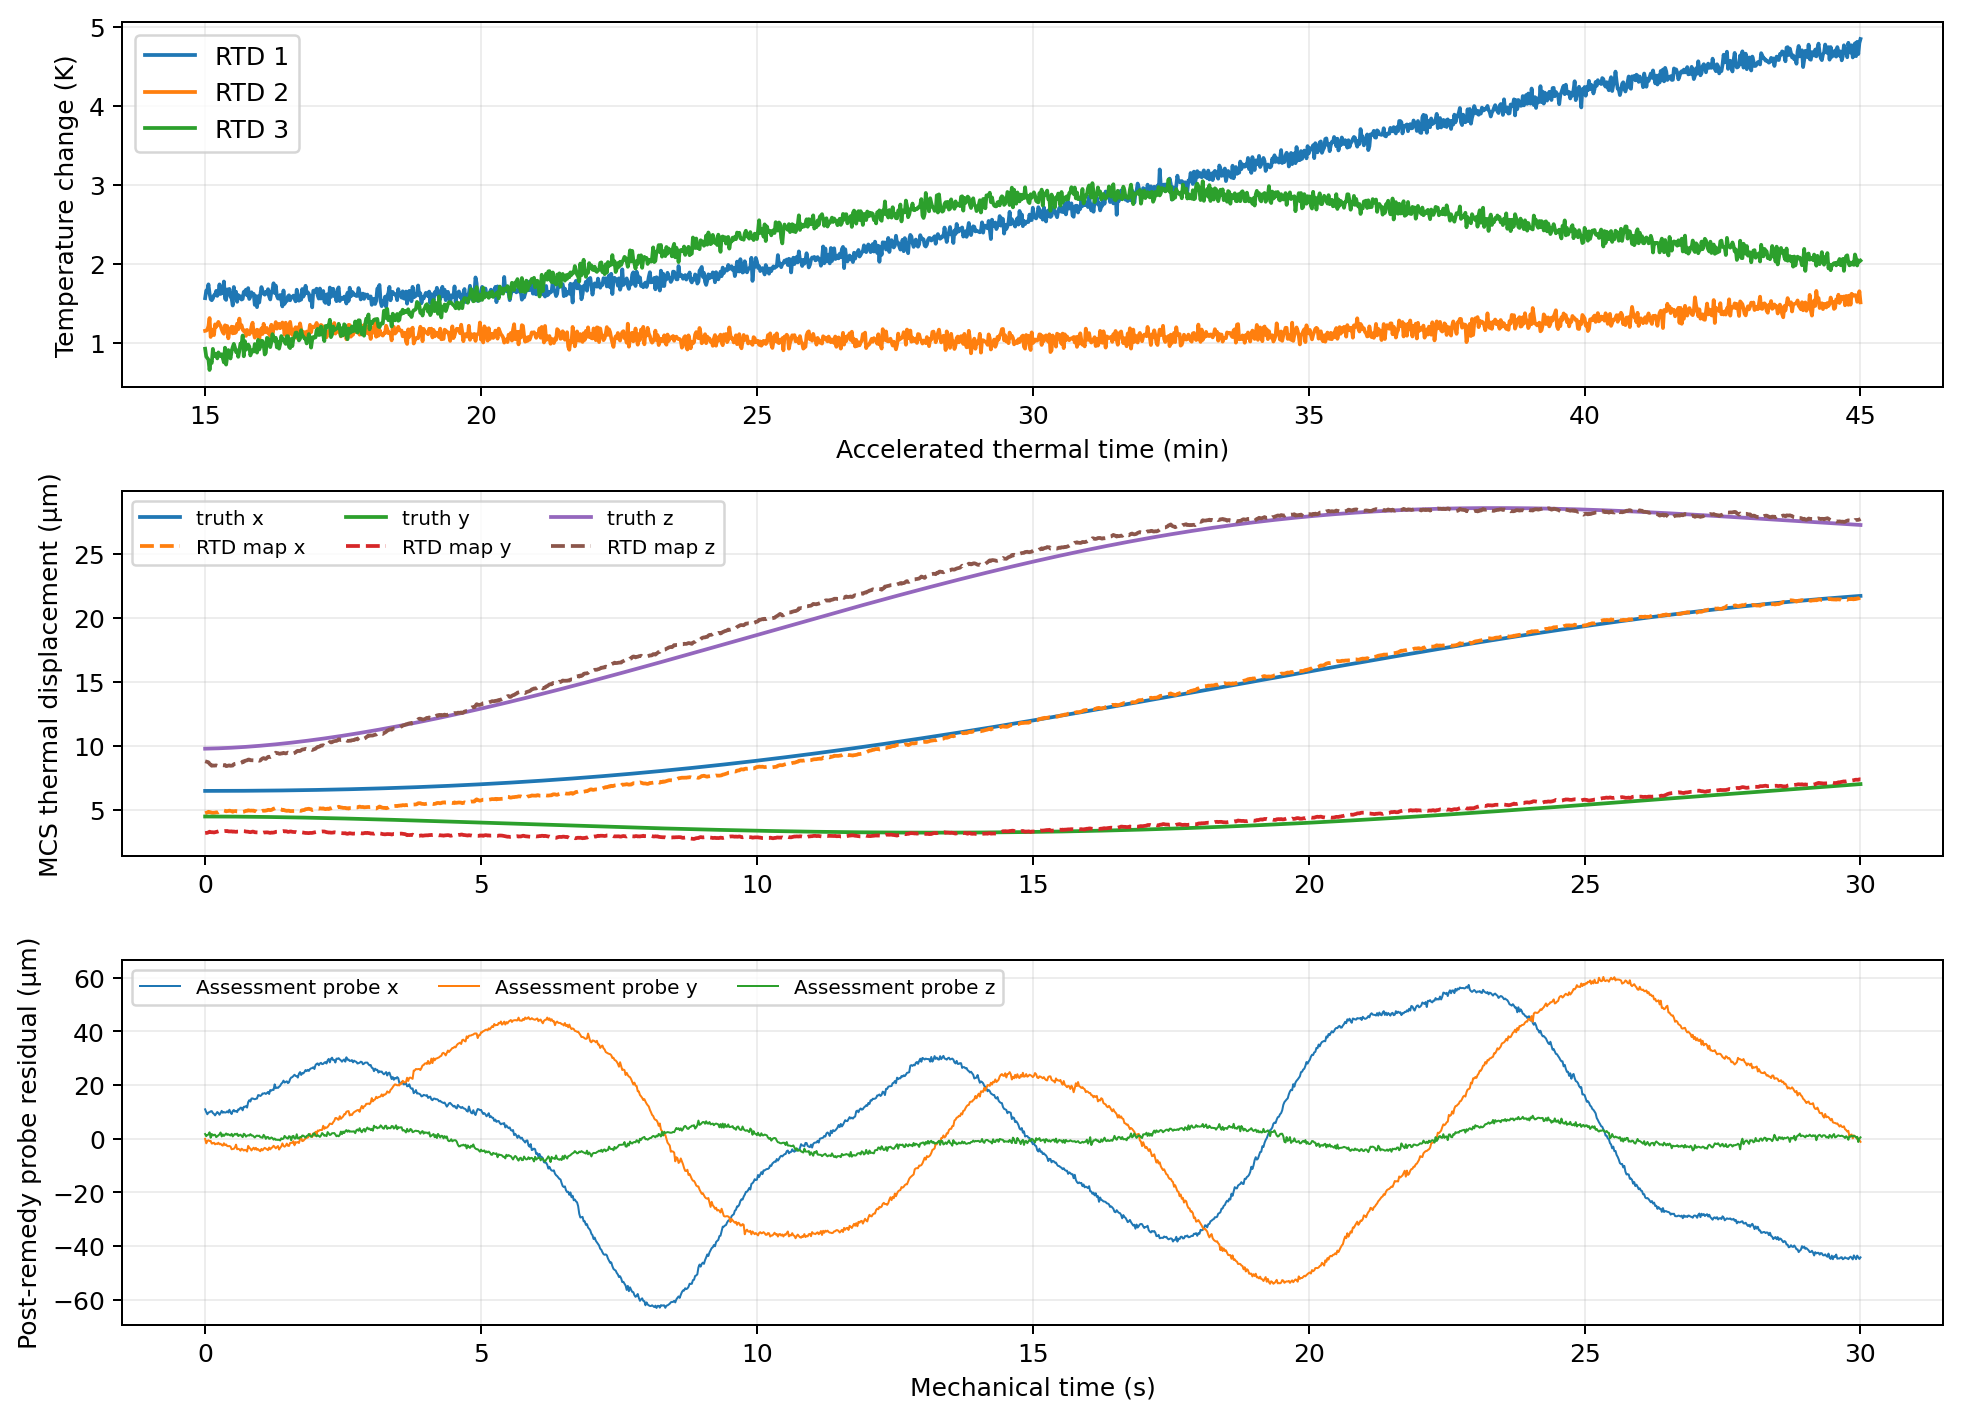
\includegraphics[width=.97\linewidth,height=73mm,keepaspectratio]{figures/research_thermal_sensors.png}\par\small\refstepcounter{figure}\textbf{Figure \thefigure.} Temperatures, inferred drift and independent position readout.\end{center}

\clearpage

\subsection{Two thermal clocks on a 30-second cut}

The physical-clock run advances temperature by 30 seconds during 30 seconds of motion. The accelerated run advances a 30-minute thermal scenario over those same mechanical commands. Physical-clock TCP RMS falls from 458.45 to 39.38 micrometres with all remedies. Under accelerated heating, the untreated RMS is 464.07. Separating the clocks exposes the interaction of thermal lag and feedforward.

\par{\small\textit{Implementation}\quad \file{publication_studies.py}\enspace /\enspace \file{dynamic_sim.py}}\par

\begin{center}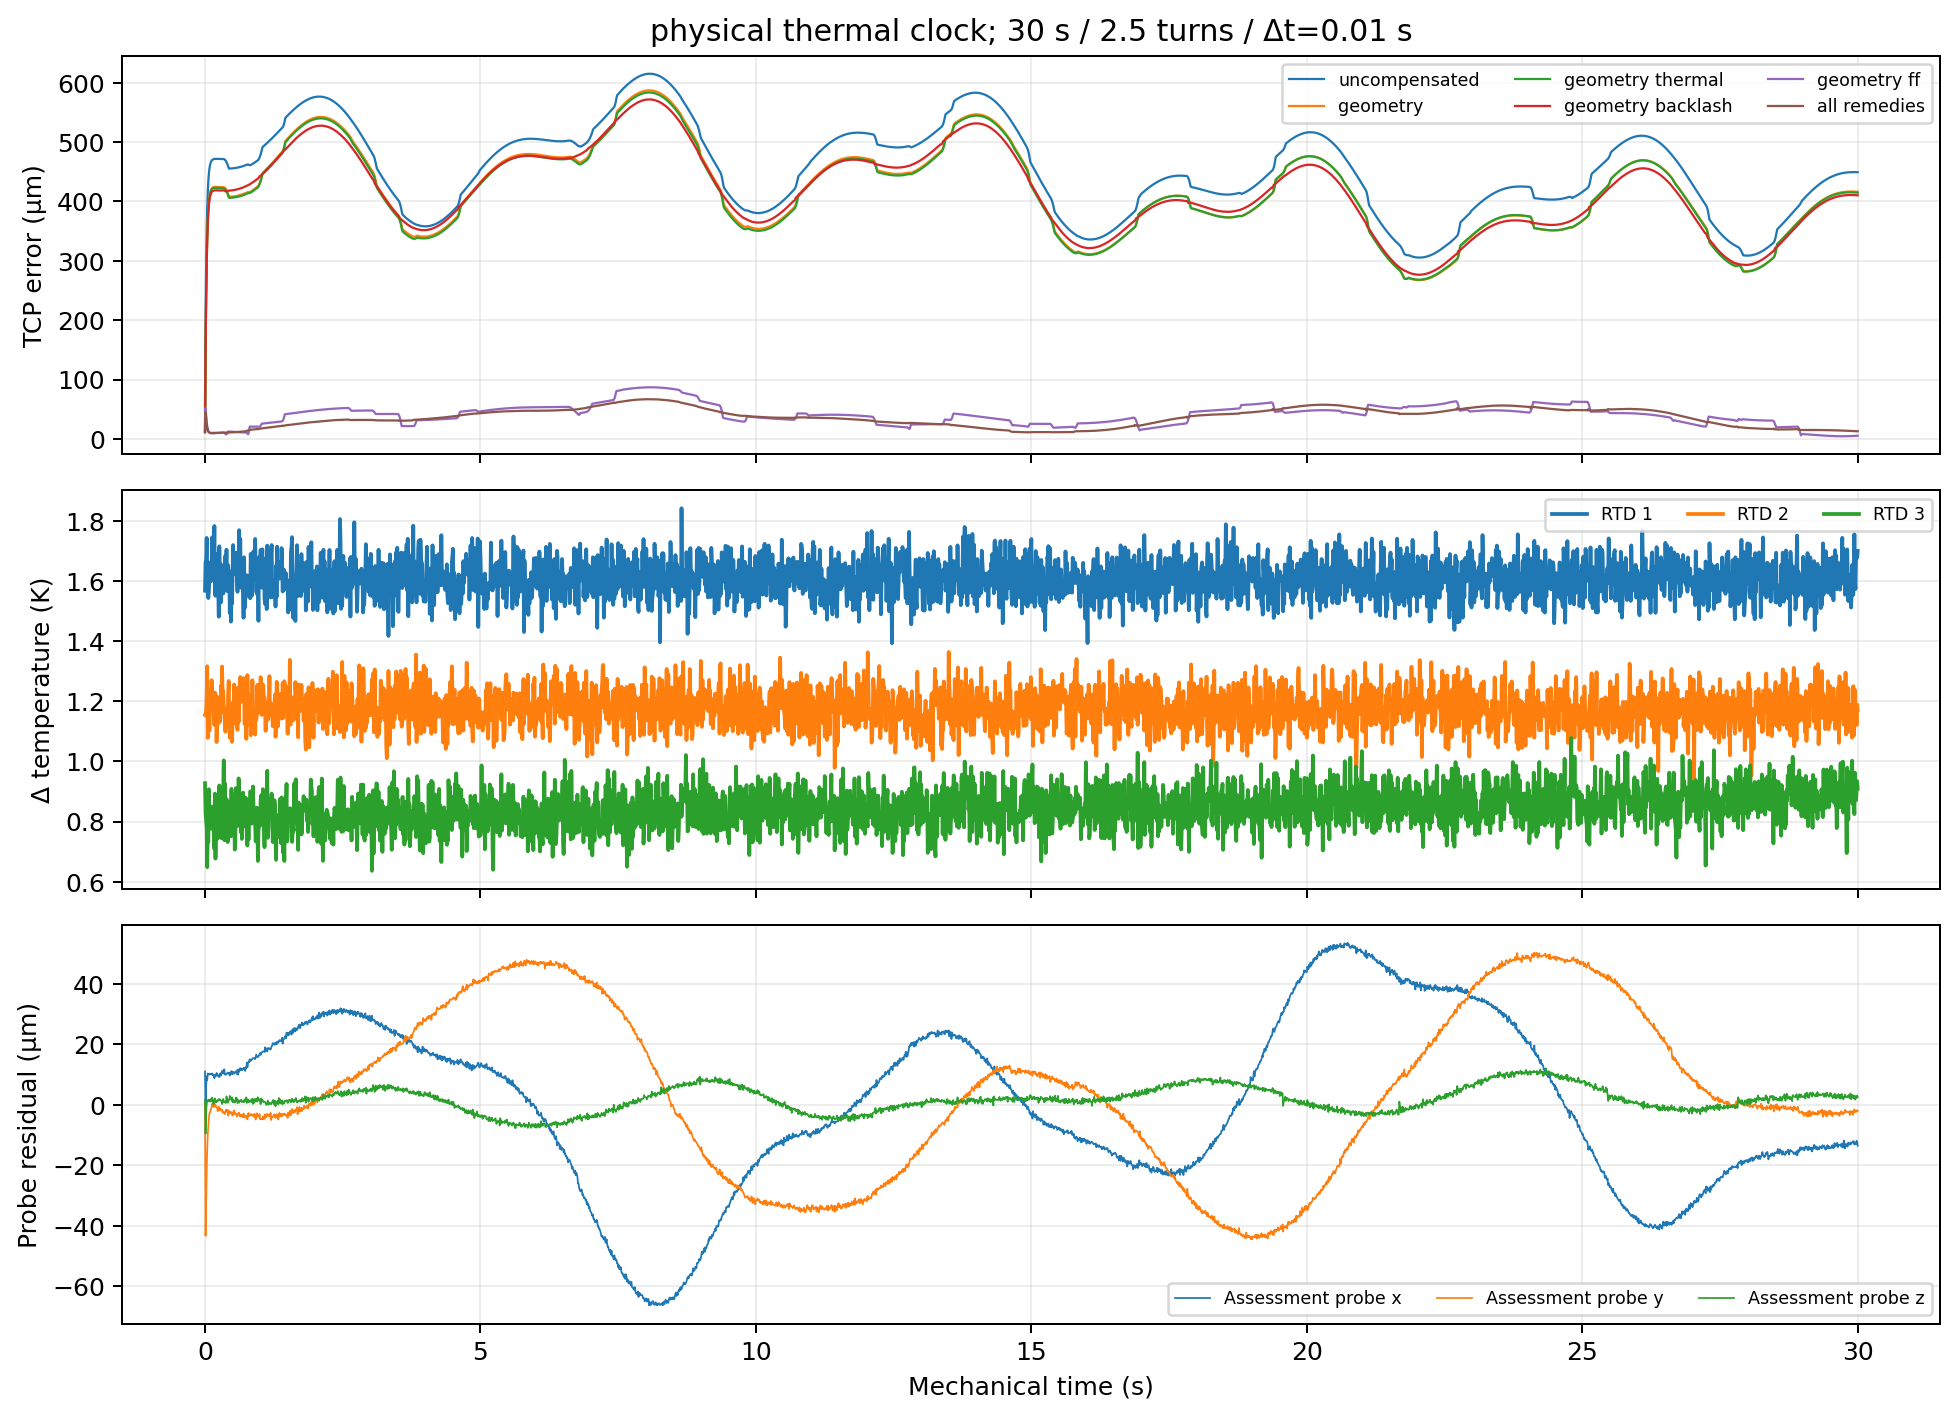
\includegraphics[width=.97\linewidth,height=73mm,keepaspectratio]{figures/publication_dynamic_physical_30.png}\par\small\refstepcounter{figure}\textbf{Figure \thefigure.} Executed path and sensor traces with physical thermal time.\end{center}

\begin{center}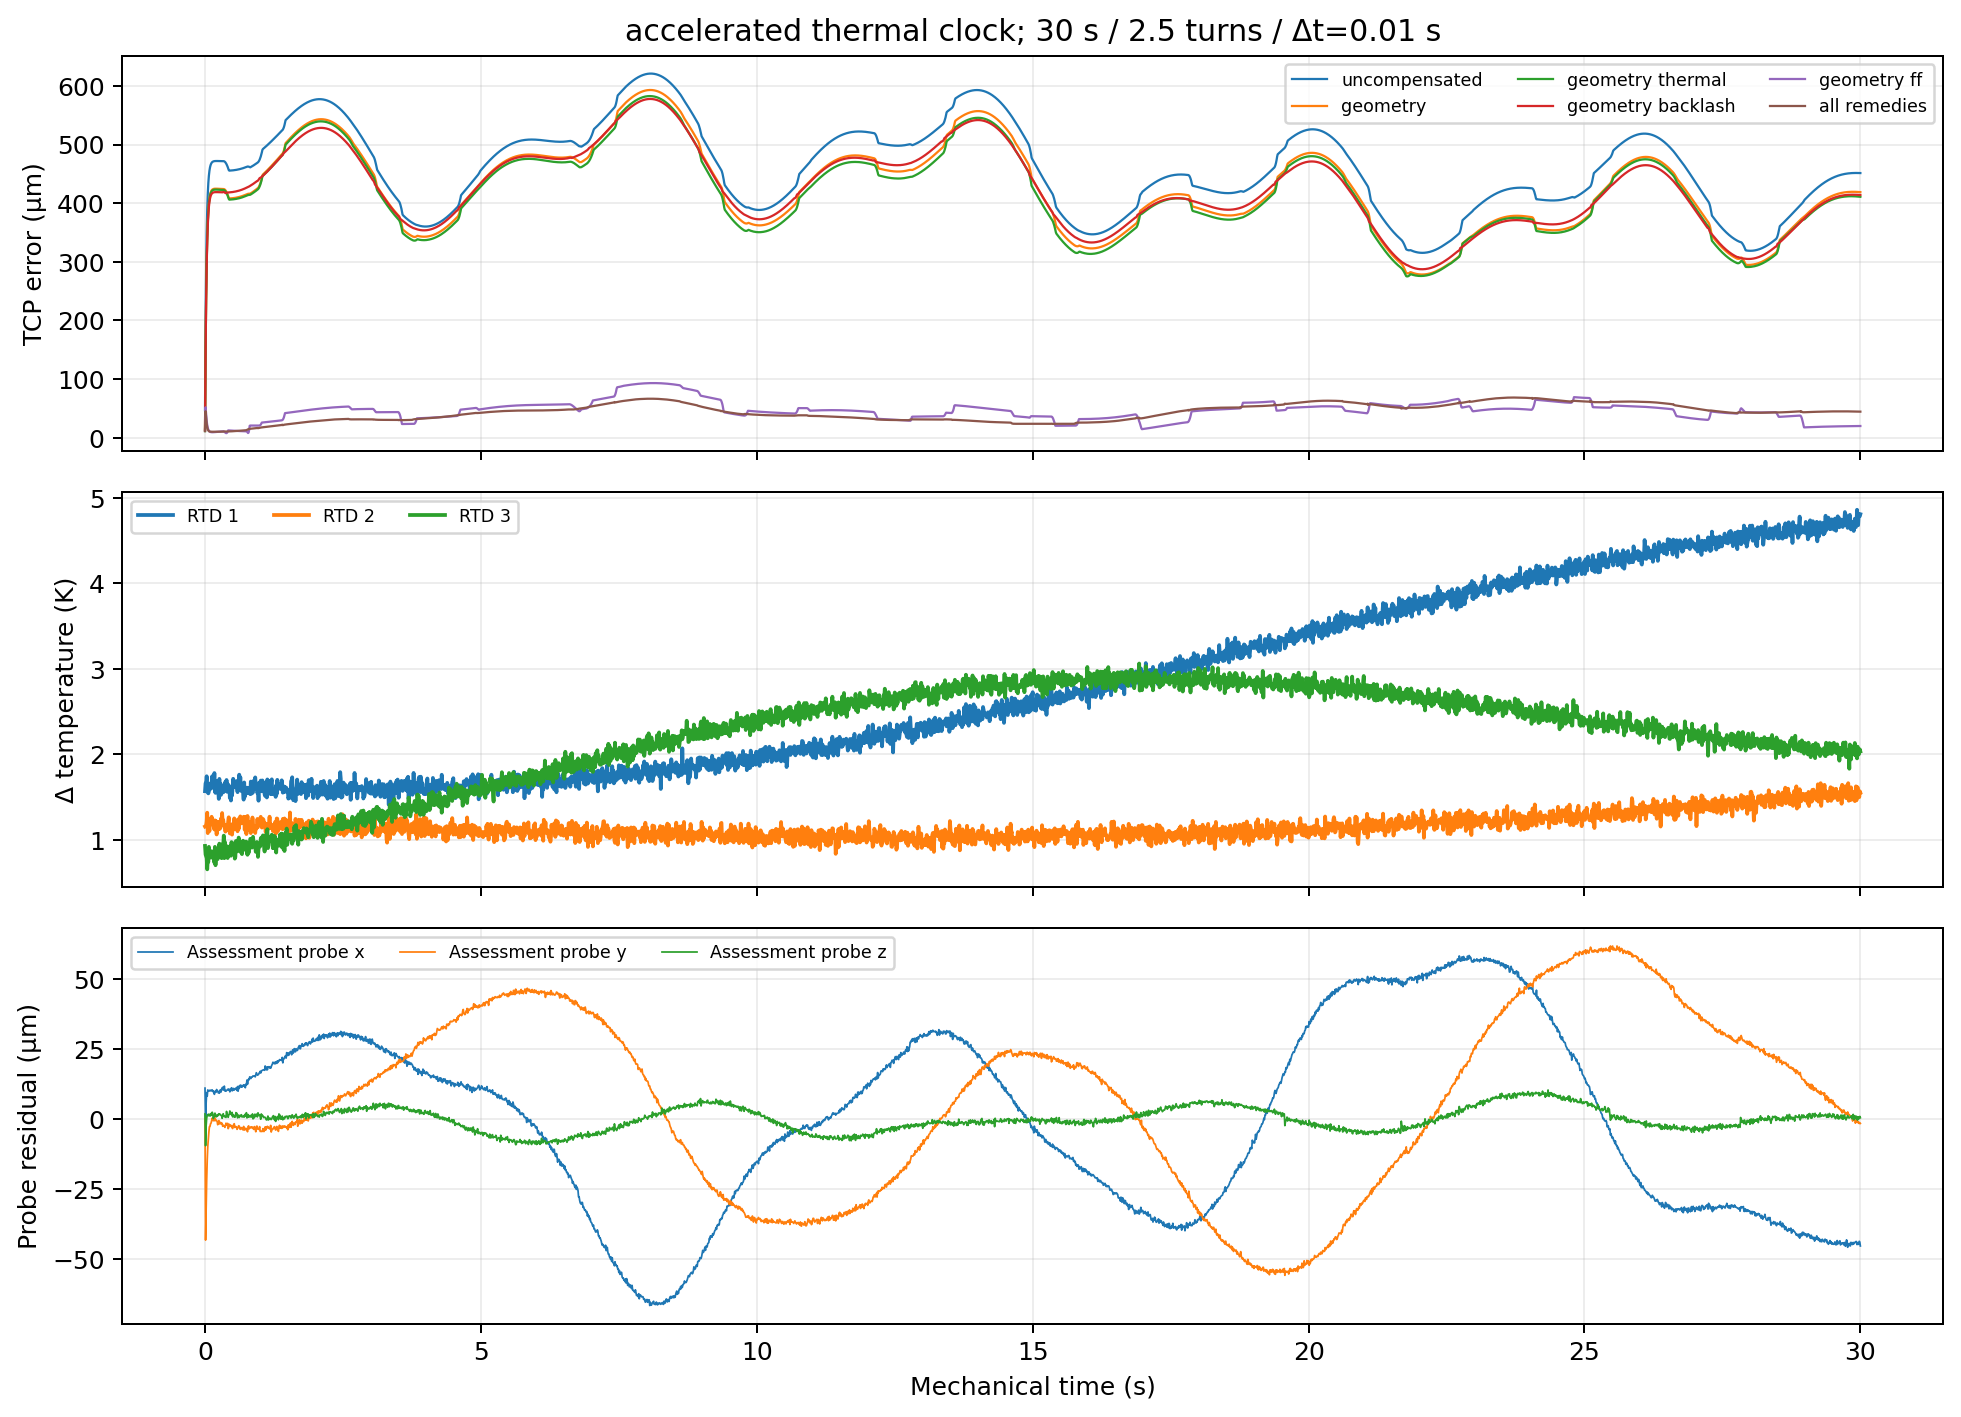
\includegraphics[width=.97\linewidth,height=73mm,keepaspectratio]{figures/publication_dynamic_accelerated_30.png}\par\small\refstepcounter{figure}\textbf{Figure \thefigure.} Same motion under accelerated thermal evolution.\end{center}

\clearpage

\subsection{Checking speed and numerical resolution}

The held-out 60 s, 1.25-turn path changes the excitation while preserving the declared calibration protocol. A separate grid study fixes fitted time constants and uses nested RTD noise. As the time step is halved from 0.005 to 0.0025 s, physical-clock full-remedy TCP RMS changes from 39.431 to 39.433 micrometres in that grid test. This checks sensitivity to sampling near the stated resolution.

\par{\small\textit{Implementation}\quad \file{publication_studies.py}\enspace /\enspace \file{dynamic_sim.py}}\par

\begin{center}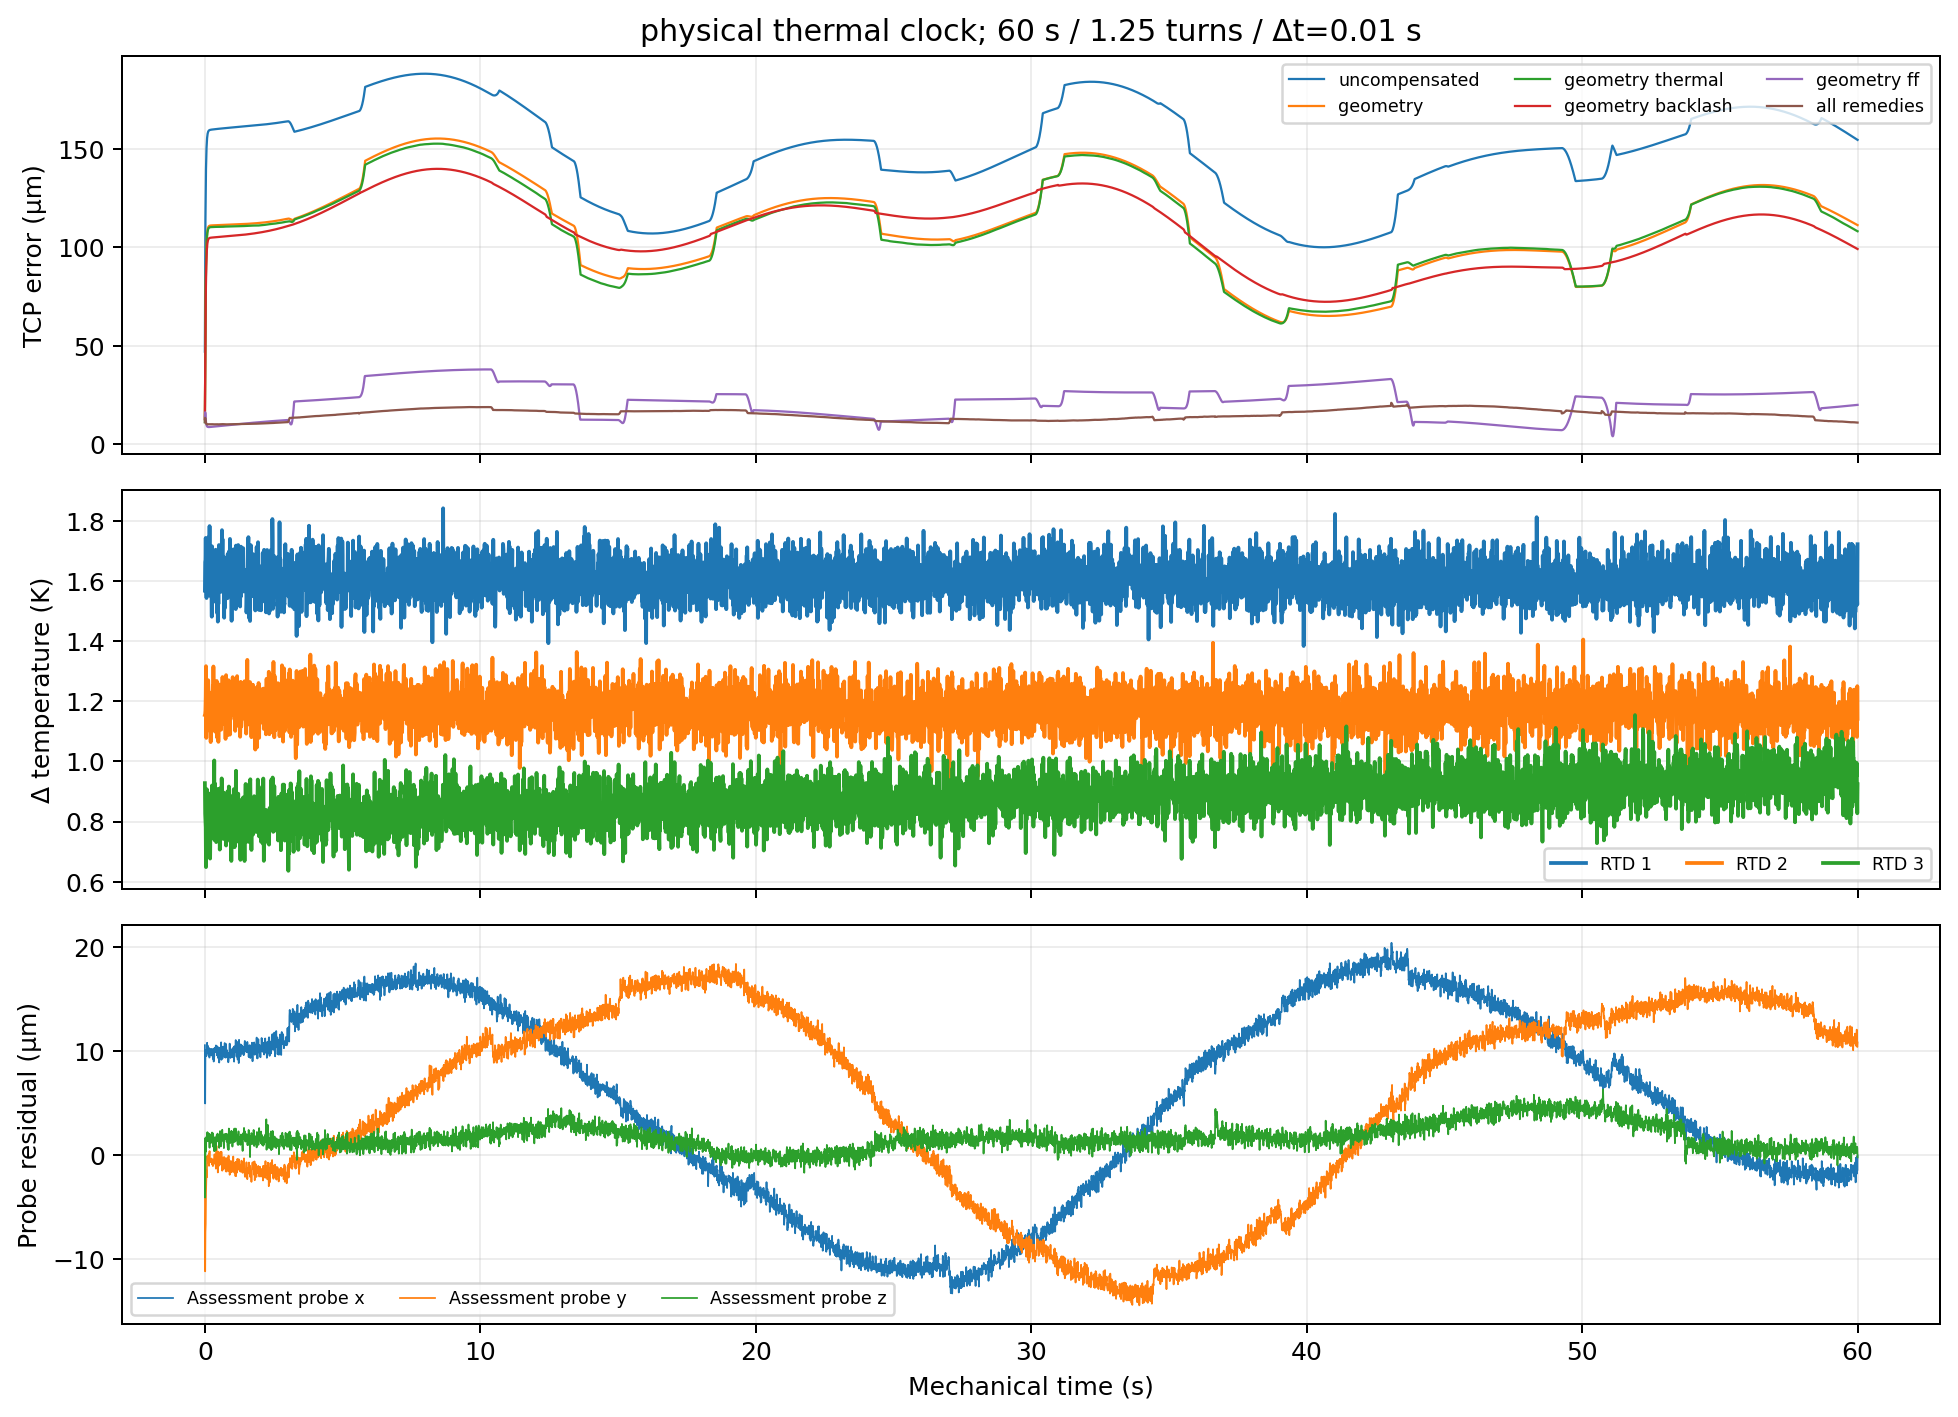
\includegraphics[width=.97\linewidth,height=47mm,keepaspectratio]{figures/publication_dynamic_physical_60.png}\par\small\refstepcounter{figure}\textbf{Figure \thefigure.} Held-out slower path with physical thermal time.\end{center}

\begin{center}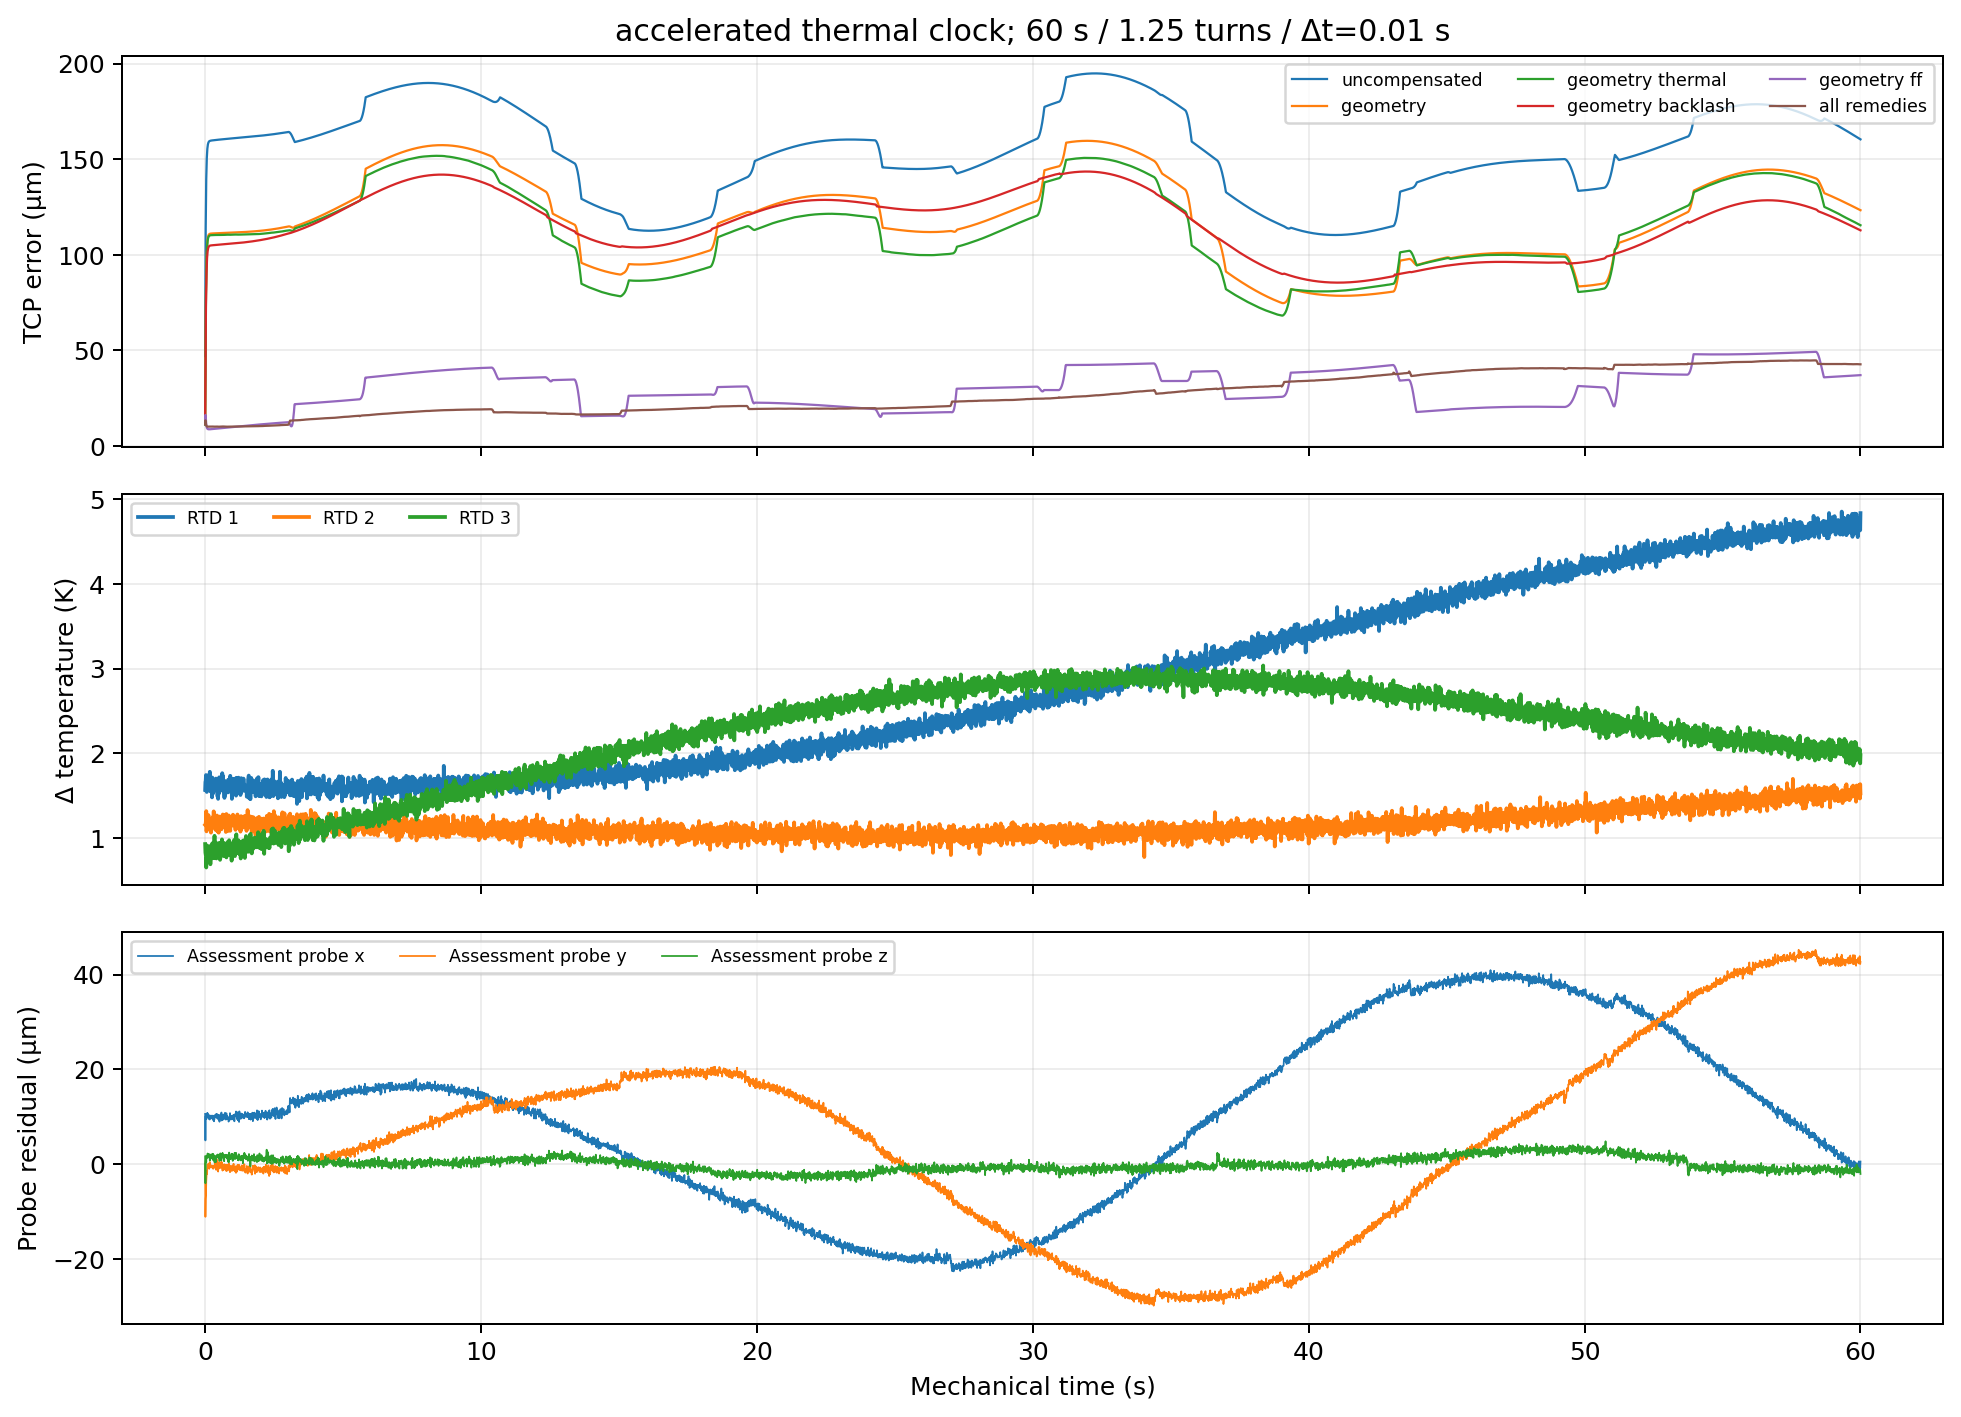
\includegraphics[width=.97\linewidth,height=47mm,keepaspectratio]{figures/publication_dynamic_accelerated_60.png}\par\small\refstepcounter{figure}\textbf{Figure \thefigure.} Slower path under accelerated thermal stress.\end{center}

\begin{center}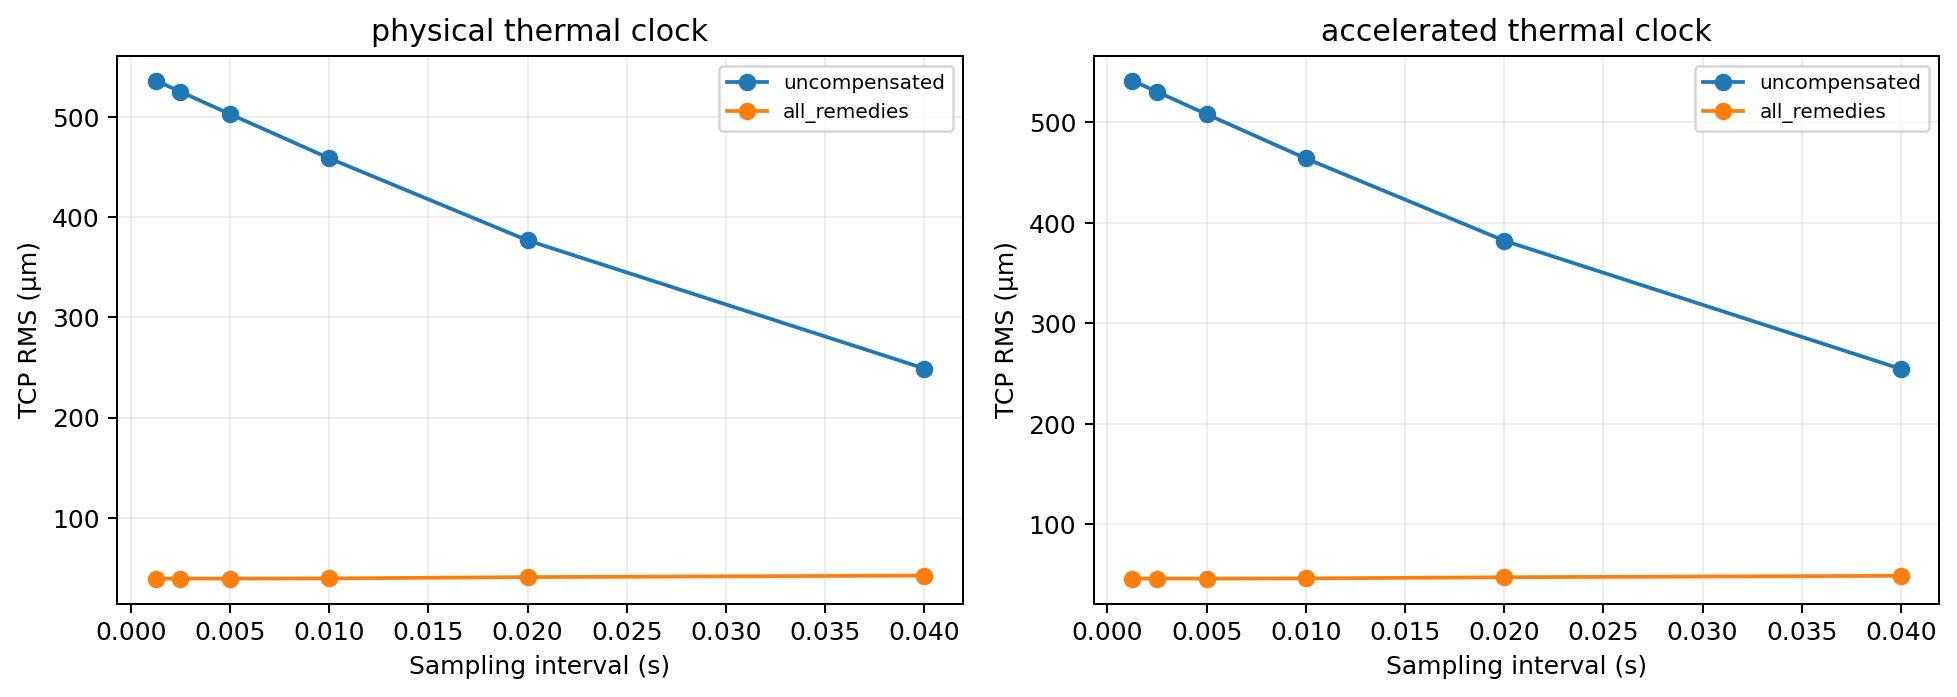
\includegraphics[width=.97\linewidth,height=47mm,keepaspectratio]{figures/publication_sampling_convergence.png}\par\small\refstepcounter{figure}\textbf{Figure \thefigure.} Discretization sensitivity of TCP and contour residuals.\end{center}

\clearpage

\section{Predictive uncertainty and inspection evidence}

\subsection{What a covariance check validates}

The first control draws noise from the same linear model used to calculate uncertainty. Agreement establishes that the propagation works under its assumptions. Repeating the experiment with independent nonlinear truth reveals a separate source of error: a bias can move the residual distribution away from zero while its spread remains small. Refining the covariance alone then leaves many observations outside the predicted region.

\par{\small\textit{Implementation}\quad \file{publication_studies.py}\enspace /\enspace \file{journal_models.py}}\par

\begin{center}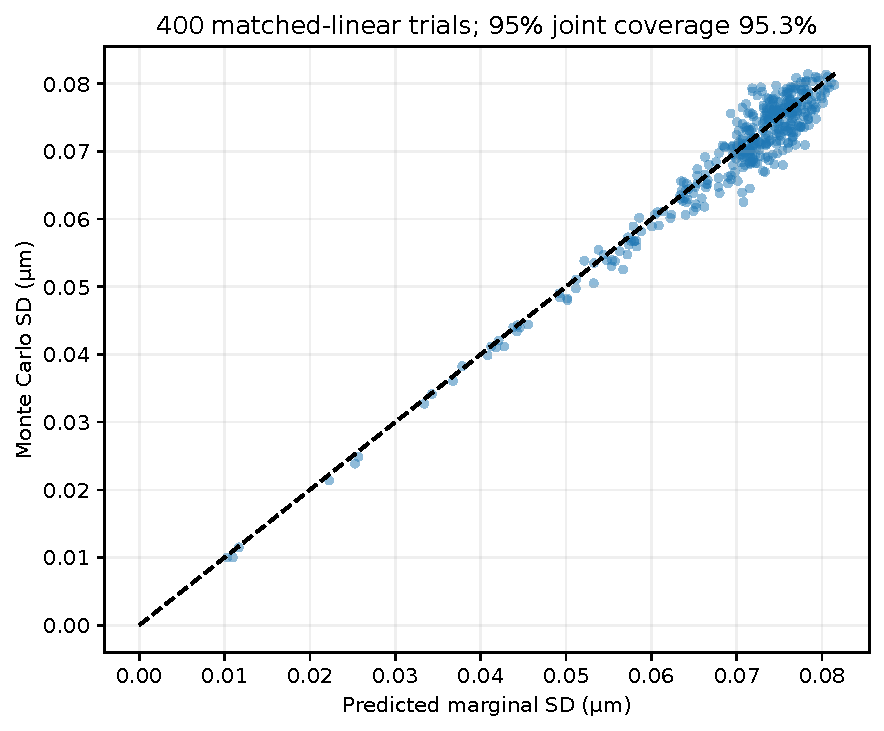
\includegraphics[width=.97\linewidth,height=73mm,keepaspectratio]{figures/publication_uncertainty_control.pdf}\par\small\refstepcounter{figure}\textbf{Figure \thefigure.} Conditional covariance compared with 400 matched-model Monte Carlo draws.\end{center}

\begin{center}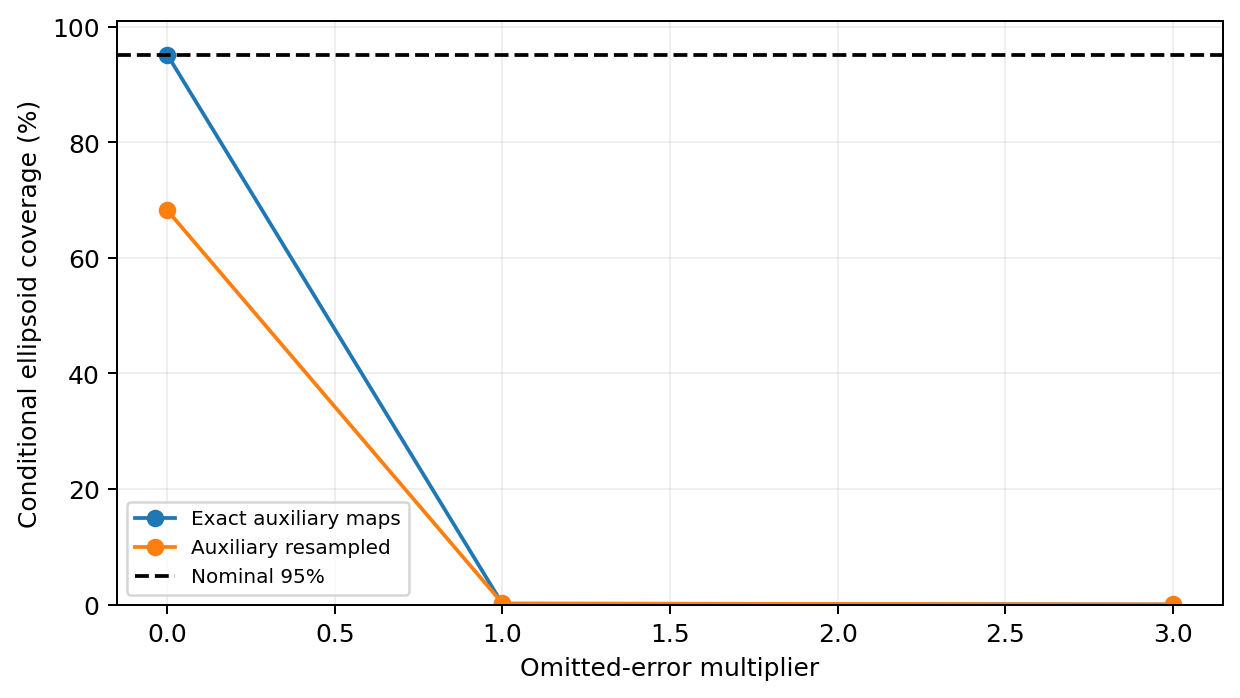
\includegraphics[width=.97\linewidth,height=73mm,keepaspectratio]{figures/publication_mismatch_coverage.png}\par\small\refstepcounter{figure}\textbf{Figure \thefigure.} Loss of coverage under omitted terms and auxiliary uncertainty.\end{center}

\clearpage

\subsection{Noise-free tool position versus a future probe reading}

In the earlier 3,600-fit audit, rotary-only propagation covers 56.13\% of matched latent TCPs; retaining shared auxiliary uncertainty gives 95.56\%. Including probe variance gives 94.97\% for the observed response. The assessment trace shows one coordinate projection. Joint coverage requires the full three-dimensional residual to fall in the ellipsoid, so counting points inside an X band overstates what that projection can establish.

\par{\small\textit{Implementation}\quad \file{journal_studies.py}\enspace /\enspace \file{journal_dashboard.py}}\par

\begin{center}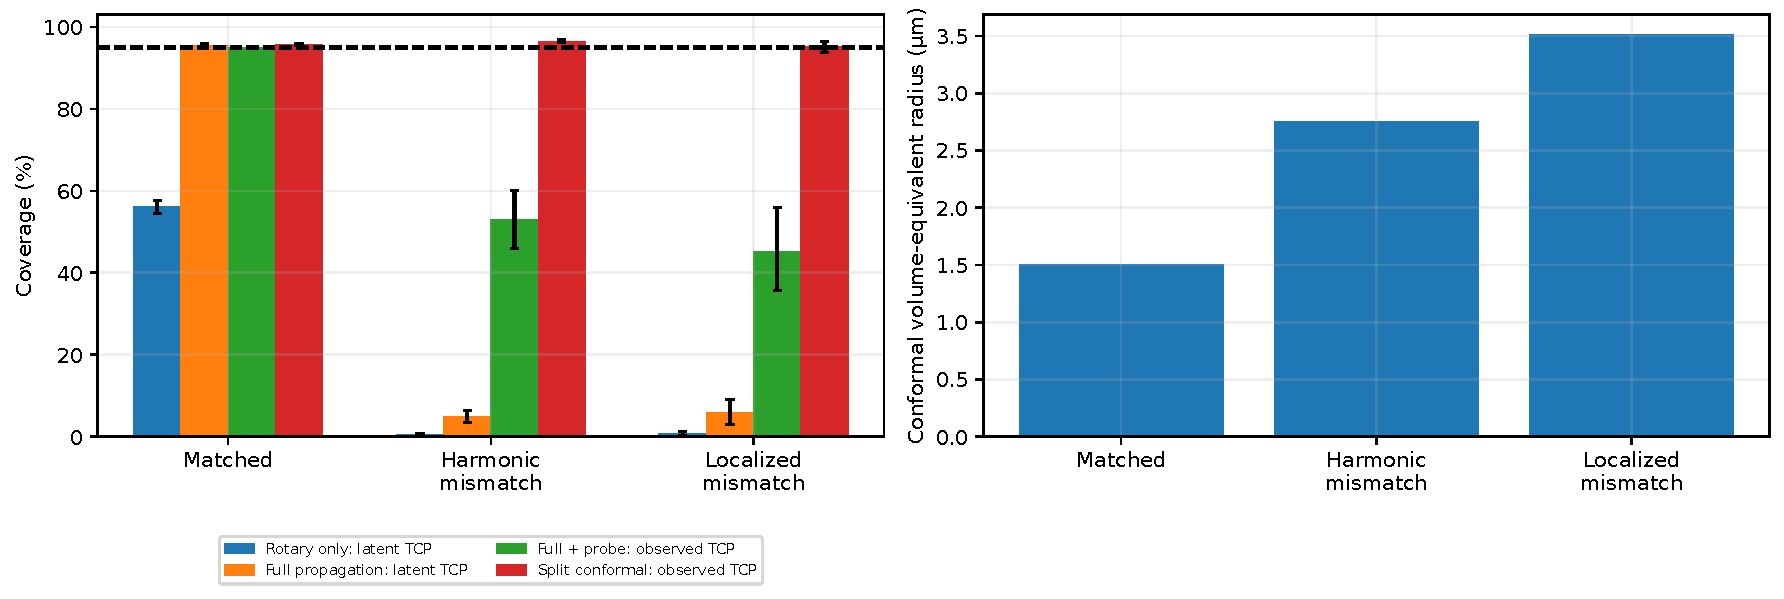
\includegraphics[width=.97\linewidth,height=73mm,keepaspectratio]{figures/journal_tcp_coverage.pdf}\par\small\refstepcounter{figure}\textbf{Figure \thefigure.} Latent and observed-target coverage in the earlier audit.\end{center}

\begin{center}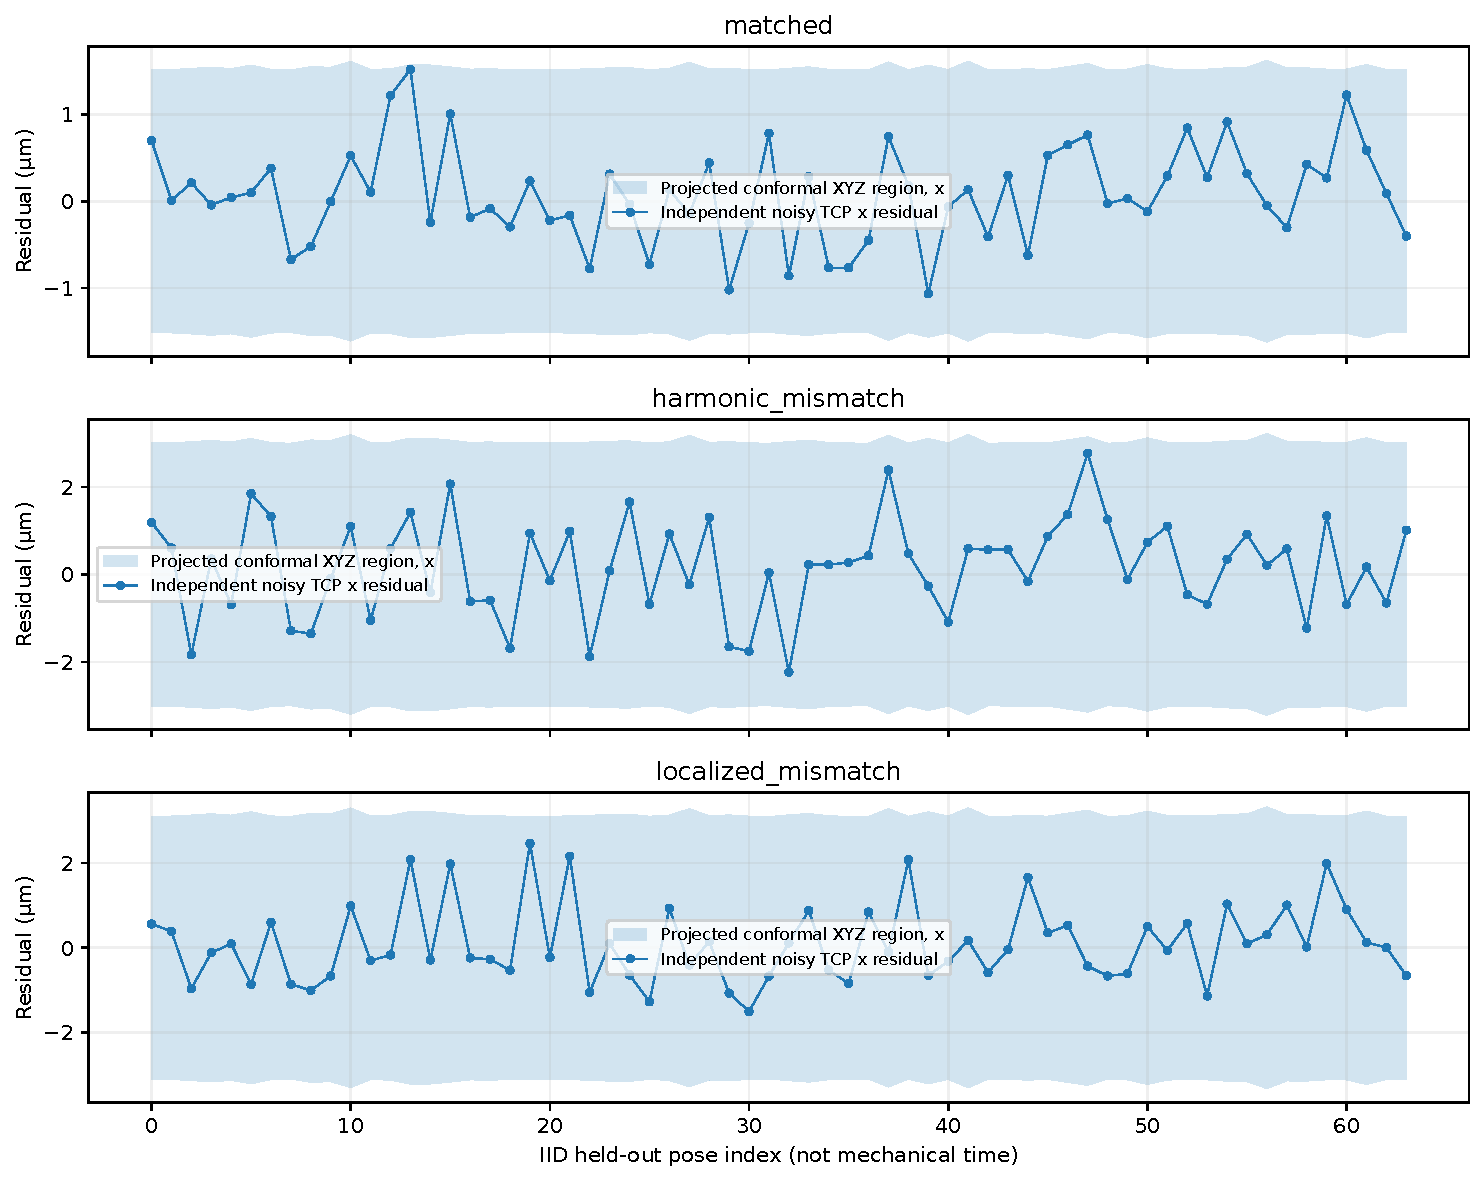
\includegraphics[width=.97\linewidth,height=73mm,keepaspectratio]{figures/journal_prediction_regions.pdf}\par\small\refstepcounter{figure}\textbf{Figure \thefigure.} X residuals and projected XYZ regions for independently drawn commands.\end{center}

\clearpage

\subsection{Comparing seven predictive regions}

The seven methods share fitted positions and assessment responses. Deleting only the fitted cross-covariance while preserving both marginal blocks raises matched independent-noise coverage to 98.05\% and mean radius from 1.449 to 1.651 micrometres. The nonlinear covariance differs from the joint first-order one by 5.82\% in relative Frobenius norm on average; the two half-samples differ by 11.29\%. The probe variance contributes to the close agreement of the Gaussian coverage values.

\par{\small\textit{Implementation}\quad \file{audit_models.py}\enspace /\enspace \file{audit_studies.py}}\par

\begin{center}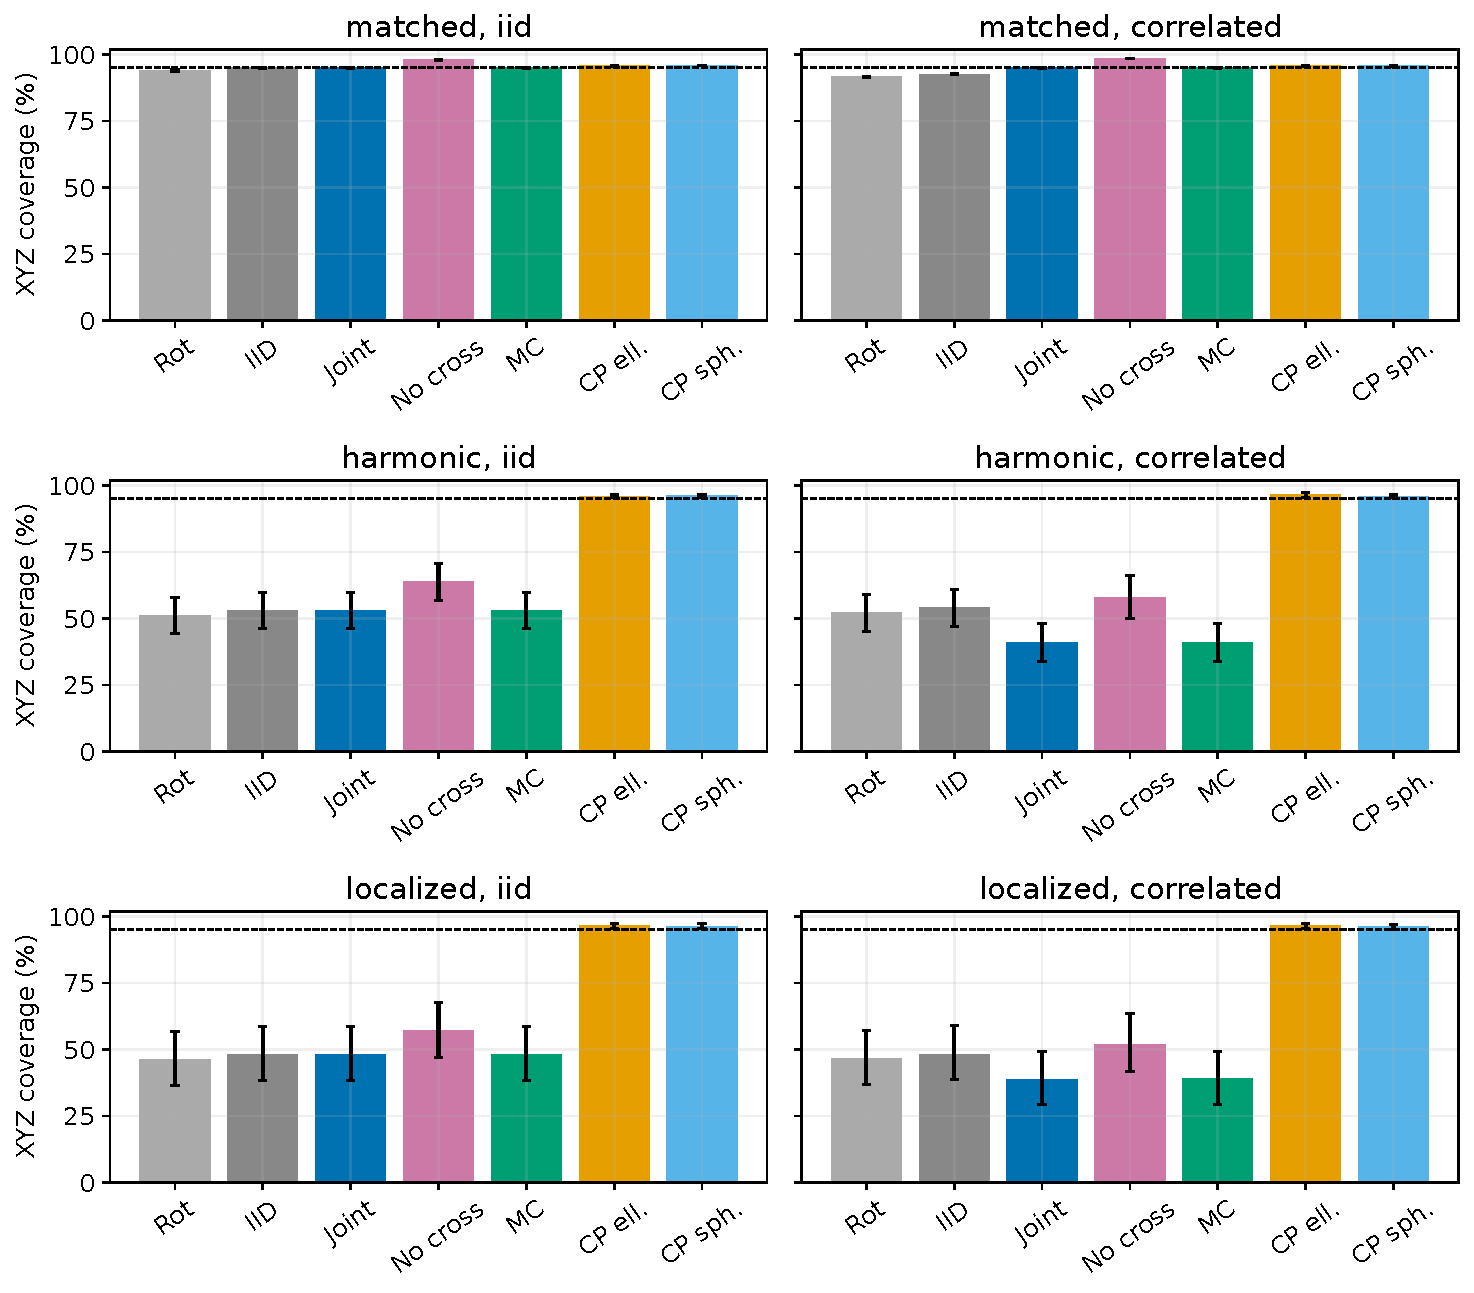
\includegraphics[width=.97\linewidth,height=73mm,keepaspectratio]{figures/audit_region_comparison.pdf}\par\small\refstepcounter{figure}\textbf{Figure \thefigure.} Seven coverage estimates for each family and noise law.\end{center}

\begin{center}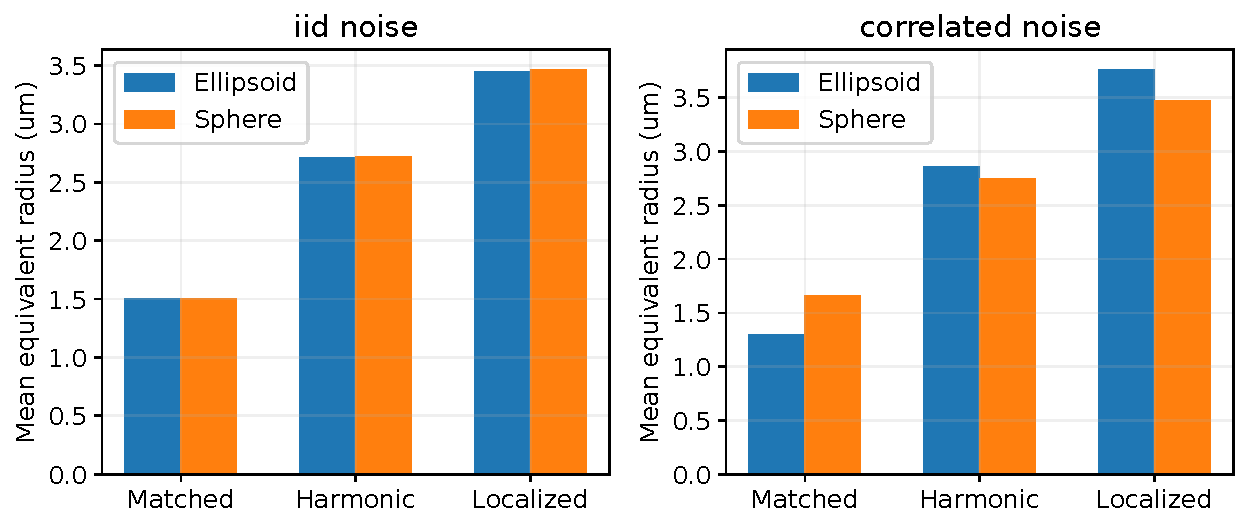
\includegraphics[width=.97\linewidth,height=73mm,keepaspectratio]{figures/audit_region_efficiency.pdf}\par\small\refstepcounter{figure}\textbf{Figure \thefigure.} Equivalent radius for the two response-calibrated shapes.\end{center}

\clearpage

\subsection{State shift and inspection replay}

Fresh calibration measures 96 responses at the original reference poses after adding a fixed displacement. It widens the prediction region while leaving the displacement in place. A complementary inspection replay freezes the normal threshold and marks anomalous responses. A missing vector triggers the acquisition-quality flag before statistical interpretation. The replay plot locates injected spikes in command space; the plotted pose index does not give elapsed time.

\par{\small\textit{Implementation}\quad \file{audit_studies.py}\enspace /\enspace \file{inspection_dashboard.py}}\par

\begin{center}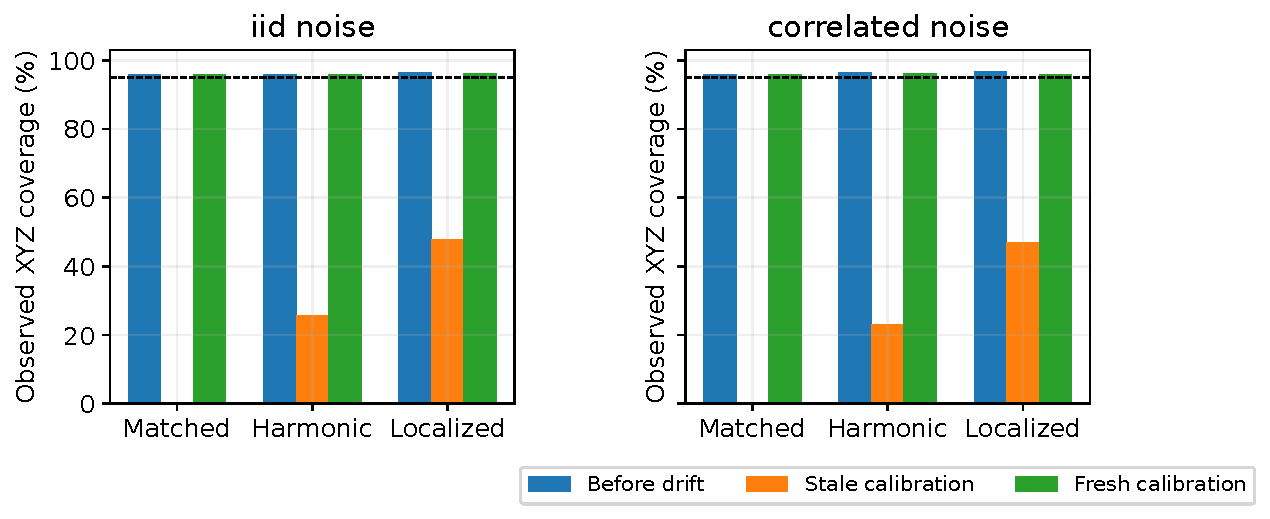
\includegraphics[width=.97\linewidth,height=73mm,keepaspectratio]{figures/audit_drift_coverage.pdf}\par\small\refstepcounter{figure}\textbf{Figure \thefigure.} Before shift, stale calibration and fresh response calibration.\end{center}

\begin{center}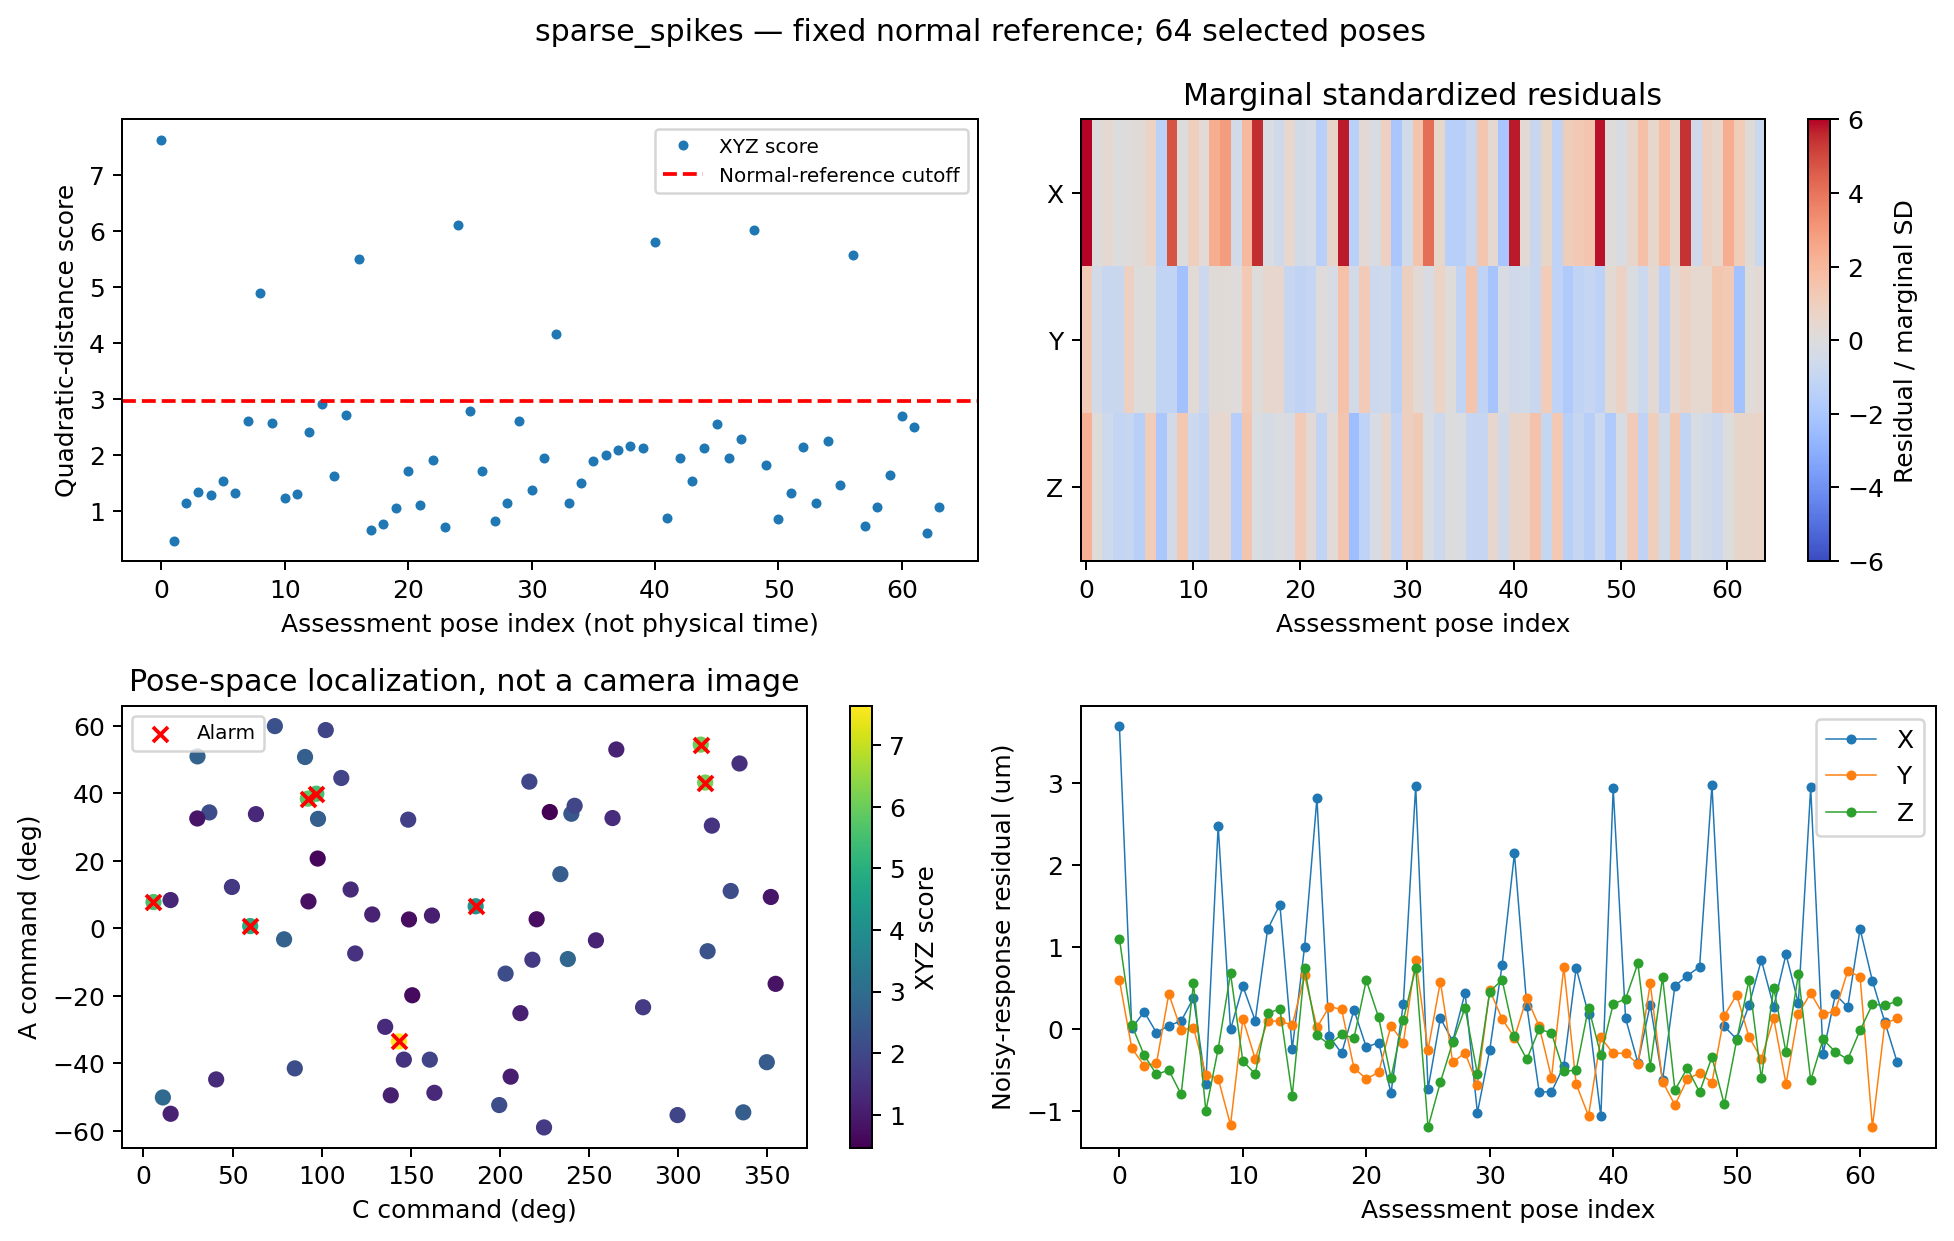
\includegraphics[width=.97\linewidth,height=73mm,keepaspectratio]{figures/inspection_spike_example.png}\par\small\refstepcounter{figure}\textbf{Figure \thefigure.} Stored sparse-spike example with score, standardized residuals and command-space location.\end{center}